\documentclass[twoside]{book}

% Packages required by doxygen
\usepackage{fixltx2e}
\usepackage{calc}
\usepackage{doxygen}
\usepackage[export]{adjustbox} % also loads graphicx
\usepackage{graphicx}
\usepackage[utf8]{inputenc}
\usepackage{makeidx}
\usepackage{multicol}
\usepackage{multirow}
\PassOptionsToPackage{warn}{textcomp}
\usepackage{textcomp}
\usepackage[nointegrals]{wasysym}
\usepackage[table]{xcolor}

% Font selection
\usepackage[T1]{fontenc}
\usepackage[scaled=.90]{helvet}
\usepackage{courier}
\usepackage{amssymb}
\usepackage{sectsty}
\renewcommand{\familydefault}{\sfdefault}
\allsectionsfont{%
  \fontseries{bc}\selectfont%
  \color{darkgray}%
}
\renewcommand{\DoxyLabelFont}{%
  \fontseries{bc}\selectfont%
  \color{darkgray}%
}
\newcommand{\+}{\discretionary{\mbox{\scriptsize$\hookleftarrow$}}{}{}}

% Page & text layout
\usepackage{geometry}
\geometry{%
  a4paper,%
  top=2.5cm,%
  bottom=2.5cm,%
  left=2.5cm,%
  right=2.5cm%
}
\tolerance=750
\hfuzz=15pt
\hbadness=750
\setlength{\emergencystretch}{15pt}
\setlength{\parindent}{0cm}
\setlength{\parskip}{3ex plus 2ex minus 2ex}
\makeatletter
\renewcommand{\paragraph}{%
  \@startsection{paragraph}{4}{0ex}{-1.0ex}{1.0ex}{%
    \normalfont\normalsize\bfseries\SS@parafont%
  }%
}
\renewcommand{\subparagraph}{%
  \@startsection{subparagraph}{5}{0ex}{-1.0ex}{1.0ex}{%
    \normalfont\normalsize\bfseries\SS@subparafont%
  }%
}
\makeatother

% Headers & footers
\usepackage{fancyhdr}
\pagestyle{fancyplain}
\fancyhead[LE]{\fancyplain{}{\bfseries\thepage}}
\fancyhead[CE]{\fancyplain{}{}}
\fancyhead[RE]{\fancyplain{}{\bfseries\leftmark}}
\fancyhead[LO]{\fancyplain{}{\bfseries\rightmark}}
\fancyhead[CO]{\fancyplain{}{}}
\fancyhead[RO]{\fancyplain{}{\bfseries\thepage}}
\fancyfoot[LE]{\fancyplain{}{}}
\fancyfoot[CE]{\fancyplain{}{}}
\fancyfoot[RE]{\fancyplain{}{\bfseries\scriptsize Generated by Doxygen }}
\fancyfoot[LO]{\fancyplain{}{\bfseries\scriptsize Generated by Doxygen }}
\fancyfoot[CO]{\fancyplain{}{}}
\fancyfoot[RO]{\fancyplain{}{}}
\renewcommand{\footrulewidth}{0.4pt}
\renewcommand{\chaptermark}[1]{%
  \markboth{#1}{}%
}
\renewcommand{\sectionmark}[1]{%
  \markright{\thesection\ #1}%
}

% Indices & bibliography
\usepackage{natbib}
\usepackage[titles]{tocloft}
\setcounter{tocdepth}{3}
\setcounter{secnumdepth}{5}
\makeindex

% Hyperlinks (required, but should be loaded last)
\usepackage{ifpdf}
\ifpdf
  \usepackage[pdftex,pagebackref=true]{hyperref}
\else
  \usepackage[ps2pdf,pagebackref=true]{hyperref}
\fi
\hypersetup{%
  colorlinks=true,%
  linkcolor=blue,%
  citecolor=blue,%
  unicode%
}

% Custom commands
\newcommand{\clearemptydoublepage}{%
  \newpage{\pagestyle{empty}\cleardoublepage}%
}

\usepackage{caption}
\captionsetup{labelsep=space,justification=centering,font={bf},singlelinecheck=off,skip=4pt,position=top}

%===== C O N T E N T S =====

\begin{document}

% Titlepage & ToC
\hypersetup{pageanchor=false,
             bookmarksnumbered=true,
             pdfencoding=unicode
            }
\pagenumbering{roman}
\begin{titlepage}
\vspace*{7cm}
\begin{center}%
{\Large 3D Game Programming Project \\[1ex]\large 0.\+1 }\\
\vspace*{1cm}
{\large Generated by Doxygen 1.8.11}\\
\end{center}
\end{titlepage}
\clearemptydoublepage
\tableofcontents
\clearemptydoublepage
\pagenumbering{arabic}
\hypersetup{pageanchor=true}

%--- Begin generated contents ---
\chapter{Todo List}
\label{todo}
\hypertarget{todo}{}

\begin{DoxyRefList}
\item[\label{todo__todo000015}%
\hypertarget{todo__todo000015}{}%
Member \hyperlink{class_ogre_1_1_dot_scene_loader_aefaa396728cce85e9bd16cbeda458b52}{Ogre\+:\+:Dot\+Scene\+Loader\+:\+:parse\+Quaternion} (Ti\+Xml\+Element $\ast$\+X\+M\+L\+Node)]Fix this crap!  
\item[\label{todo__todo000012}%
\hypertarget{todo__todo000012}{}%
Member \hyperlink{class_ogre_1_1_dot_scene_loader_a9b7c7ccd8f2724eb44dc9428ba6cb0d7}{Ogre\+:\+:Dot\+Scene\+Loader\+:\+:process\+Billboard\+Set} (Ti\+Xml\+Element $\ast$\+X\+M\+L\+Node, Scene\+Node $\ast$p\+Parent)]Implement this  
\item[\label{todo__todo000006}%
\hypertarget{todo__todo000006}{}%
Member \hyperlink{class_ogre_1_1_dot_scene_loader_a92989e4631cd46d31337c006b46c1aea}{Ogre\+:\+:Dot\+Scene\+Loader\+:\+:process\+Camera} (Ti\+Xml\+Element $\ast$\+X\+M\+L\+Node, Scene\+Node $\ast$p\+Parent=0)]Is this always in degrees? 

What to do with this element? 

Implement the camera look target 

Implement the camera track target 

Implement the camera user data reference  
\item[\label{todo__todo000014}%
\hypertarget{todo__todo000014}{}%
Member \hyperlink{class_ogre_1_1_dot_scene_loader_a0d8466f519cf49e4177369b542da50be}{Ogre\+:\+:Dot\+Scene\+Loader\+:\+:process\+Clipping} (Ti\+Xml\+Element $\ast$\+X\+M\+L\+Node)]Implement this  
\item[\label{todo__todo000002}%
\hypertarget{todo__todo000002}{}%
Member \hyperlink{class_ogre_1_1_dot_scene_loader_a6c541dcb42d29071b2556b85f8cd1a62}{Ogre\+:\+:Dot\+Scene\+Loader\+:\+:process\+Environment} (Ti\+Xml\+Element $\ast$\+X\+M\+L\+Node)]Set the background colour of all viewports (Render\+Window has to be provided then)  
\item[\label{todo__todo000001}%
\hypertarget{todo__todo000001}{}%
Member \hyperlink{class_ogre_1_1_dot_scene_loader_a1627804a409b0dccd5598323f3d85359}{Ogre\+:\+:Dot\+Scene\+Loader\+:\+:process\+Externals} (Ti\+Xml\+Element $\ast$\+X\+M\+L\+Node)]Implement this  
\item[\label{todo__todo000011}%
\hypertarget{todo__todo000011}{}%
Member \hyperlink{class_ogre_1_1_dot_scene_loader_a3f8227871f6a283222b1d0a88076d6d8}{Ogre\+:\+:Dot\+Scene\+Loader\+:\+:process\+Look\+Target} (Ti\+Xml\+Element $\ast$\+X\+M\+L\+Node, Scene\+Node $\ast$p\+Parent)]Is this correct? Cause I don\textquotesingle{}t have a clue actually  
\item[\label{todo__todo000005}%
\hypertarget{todo__todo000005}{}%
Member \hyperlink{class_ogre_1_1_dot_scene_loader_ad23d30b2c6ee9d24dabc89b28d9b61ed}{Ogre\+:\+:Dot\+Scene\+Loader\+:\+:process\+Octree} (Ti\+Xml\+Element $\ast$\+X\+M\+L\+Node)]Implement this  
\item[\label{todo__todo000013}%
\hypertarget{todo__todo000013}{}%
Member \hyperlink{class_ogre_1_1_dot_scene_loader_a8131406550814512ea64907b598b3f1c}{Ogre\+:\+:Dot\+Scene\+Loader\+:\+:process\+Plane} (Ti\+Xml\+Element $\ast$\+X\+M\+L\+Node, Scene\+Node $\ast$p\+Parent)]Implement this  
\item[\label{todo__todo000003}%
\hypertarget{todo__todo000003}{}%
Member \hyperlink{class_ogre_1_1_dot_scene_loader_ad2f5858edce531f9a7be2e6ebdcebc5e}{Ogre\+:\+:Dot\+Scene\+Loader\+:\+:process\+Terrain} (Ti\+Xml\+Element $\ast$\+X\+M\+L\+Node)]Implement this  
\item[\label{todo__todo000004}%
\hypertarget{todo__todo000004}{}%
Member \hyperlink{class_ogre_1_1_dot_scene_loader_a24d6db1a195dea881b934753253e8e68}{Ogre\+:\+:Dot\+Scene\+Loader\+:\+:process\+User\+Data\+Reference} (Ti\+Xml\+Element $\ast$\+X\+M\+L\+Node, Scene\+Node $\ast$p\+Parent=0)]Implement this 
\end{DoxyRefList}
\chapter{Hierarchical Index}
\section{Class Hierarchy}
This inheritance list is sorted roughly, but not completely, alphabetically\+:\begin{DoxyCompactList}
\item \contentsline{section}{Camera\+Motion}{\pageref{class_camera_motion}}{}
\item Contact\+Result\+Callback\begin{DoxyCompactList}
\item \contentsline{section}{N\+C\+TU\+:\+:Bullet\+Contact\+Result\+Callback}{\pageref{struct_n_c_t_u_1_1_bullet_contact_result_callback}}{}
\item \contentsline{section}{N\+C\+TU\+:\+:Floor\+Contact\+Result\+Callback}{\pageref{struct_n_c_t_u_1_1_floor_contact_result_callback}}{}
\item \contentsline{section}{N\+C\+TU\+:\+:Obstacle\+Contact\+Result\+Callback}{\pageref{struct_n_c_t_u_1_1_obstacle_contact_result_callback}}{}
\item \contentsline{section}{N\+C\+TU\+:\+:Pickup\+Contact\+Result\+Callback}{\pageref{struct_n_c_t_u_1_1_pickup_contact_result_callback}}{}
\end{DoxyCompactList}
\item \contentsline{section}{Ogre\+:\+:Dot\+Scene\+Loader}{\pageref{class_ogre_1_1_dot_scene_loader}}{}
\item Frame\+Listener\begin{DoxyCompactList}
\item \contentsline{section}{Base\+Application}{\pageref{class_base_application}}{}
\begin{DoxyCompactList}
\item \contentsline{section}{Basic\+Tutorial\+\_\+00}{\pageref{class_basic_tutorial__00}}{}
\end{DoxyCompactList}
\end{DoxyCompactList}
\item \contentsline{section}{Ogre\+:\+:General\+Property}{\pageref{class_ogre_1_1_general_property}}{}
\item \contentsline{section}{N\+C\+TU\+:\+:G\+U\+I\+Manager}{\pageref{class_n_c_t_u_1_1_g_u_i_manager}}{}
\item \contentsline{section}{N\+C\+TU\+:\+:G\+U\+I\+Window}{\pageref{class_n_c_t_u_1_1_g_u_i_window}}{}
\begin{DoxyCompactList}
\item \contentsline{section}{N\+C\+TU\+:\+:Game\+Console\+Window}{\pageref{class_n_c_t_u_1_1_game_console_window}}{}
\item \contentsline{section}{N\+C\+TU\+:\+:Game\+Menu\+Window}{\pageref{class_n_c_t_u_1_1_game_menu_window}}{}
\item \contentsline{section}{N\+C\+TU\+:\+:Game\+Over\+Window}{\pageref{class_n_c_t_u_1_1_game_over_window}}{}
\item \contentsline{section}{N\+C\+TU\+:\+:Level\+Menu\+Window}{\pageref{class_n_c_t_u_1_1_level_menu_window}}{}
\item \contentsline{section}{N\+C\+TU\+:\+:Main\+Menu\+Window}{\pageref{class_n_c_t_u_1_1_main_menu_window}}{}
\item \contentsline{section}{N\+C\+TU\+:\+:Score\+Bar\+Window}{\pageref{class_n_c_t_u_1_1_score_bar_window}}{}
\end{DoxyCompactList}
\item \contentsline{section}{Key\+Board\+Handler}{\pageref{class_key_board_handler}}{}
\item \contentsline{section}{Key\+Data}{\pageref{struct_key_data}}{}
\item Key\+Listener\begin{DoxyCompactList}
\item \contentsline{section}{Base\+Application}{\pageref{class_base_application}}{}
\end{DoxyCompactList}
\item map\begin{DoxyCompactList}
\item \contentsline{section}{prop\+Map$<$ Key, Value $>$}{\pageref{classprop_map}}{}
\item \contentsline{section}{prop\+Map$<$ int, Ogre\+:\+:String $>$}{\pageref{classprop_map}}{}
\item \contentsline{section}{prop\+Map$<$ int, String $>$}{\pageref{classprop_map}}{}
\item \contentsline{section}{prop\+Map$<$ String, Ogre\+:\+:General\+Property $>$}{\pageref{classprop_map}}{}
\end{DoxyCompactList}
\item Mouse\+Listener\begin{DoxyCompactList}
\item \contentsline{section}{Base\+Application}{\pageref{class_base_application}}{}
\end{DoxyCompactList}
\item \contentsline{section}{N\+C\+T\+U\+Camera}{\pageref{class_n_c_t_u_camera}}{}
\item \contentsline{section}{Ogre\+:\+:node\+Property}{\pageref{class_ogre_1_1node_property}}{}
\item \contentsline{section}{N\+C\+TU\+:\+:Obstacle}{\pageref{class_n_c_t_u_1_1_obstacle}}{}
\begin{DoxyCompactList}
\item \contentsline{section}{N\+C\+TU\+:\+:Bullet\+Obstacle}{\pageref{class_n_c_t_u_1_1_bullet_obstacle}}{}
\item \contentsline{section}{N\+C\+TU\+:\+:Cube\+Obstacle}{\pageref{class_n_c_t_u_1_1_cube_obstacle}}{}
\item \contentsline{section}{N\+C\+TU\+:\+:Floor\+Obstacle}{\pageref{class_n_c_t_u_1_1_floor_obstacle}}{}
\item \contentsline{section}{N\+C\+TU\+:\+:General\+Obstacle}{\pageref{class_n_c_t_u_1_1_general_obstacle}}{}
\item \contentsline{section}{N\+C\+TU\+:\+:Pickup\+Obstacle}{\pageref{class_n_c_t_u_1_1_pickup_obstacle}}{}
\item \contentsline{section}{N\+C\+TU\+:\+:Player\+Obstacle}{\pageref{class_n_c_t_u_1_1_player_obstacle}}{}
\item \contentsline{section}{N\+C\+TU\+:\+:Sphere\+Obstacle}{\pageref{class_n_c_t_u_1_1_sphere_obstacle}}{}
\end{DoxyCompactList}
\item \contentsline{section}{N\+C\+TU\+:\+:Obstacle\+Manager}{\pageref{class_n_c_t_u_1_1_obstacle_manager}}{}
\item \contentsline{section}{Ogre\+:\+:Obstacle\+Property}{\pageref{class_ogre_1_1_obstacle_property}}{}
\item \contentsline{section}{N\+C\+TU\+:\+:Particle\+System\+Pack}{\pageref{struct_n_c_t_u_1_1_particle_system_pack}}{}
\item Sdk\+Tray\+Listener\begin{DoxyCompactList}
\item \contentsline{section}{Base\+Application}{\pageref{class_base_application}}{}
\end{DoxyCompactList}
\item \contentsline{section}{N\+C\+TU\+:\+:Audio\+:\+:Sound\+Slot}{\pageref{struct_n_c_t_u_1_1_audio_1_1_sound_slot}}{}
\item Window\+Event\+Listener\begin{DoxyCompactList}
\item \contentsline{section}{Base\+Application}{\pageref{class_base_application}}{}
\end{DoxyCompactList}
\end{DoxyCompactList}

\chapter{Class Index}
\section{Class List}
Here are the classes, structs, unions and interfaces with brief descriptions\+:\begin{DoxyCompactList}
\item\contentsline{section}{\hyperlink{class_base_application}{Base\+Application} \\*Base class for application }{\pageref{class_base_application}}{}
\item\contentsline{section}{\hyperlink{class_basic_tutorial__00}{Basic\+Tutorial\+\_\+00} \\*Main class for the application }{\pageref{class_basic_tutorial__00}}{}
\item\contentsline{section}{\hyperlink{struct_n_c_t_u_1_1_bullet_contact_result_callback}{N\+C\+T\+U\+::\+Bullet\+Contact\+Result\+Callback} \\*Callback for bullet-\/obstacle contact }{\pageref{struct_n_c_t_u_1_1_bullet_contact_result_callback}}{}
\item\contentsline{section}{\hyperlink{class_n_c_t_u_1_1_bullet_obstacle}{N\+C\+T\+U\+::\+Bullet\+Obstacle} \\*Bullet obstacle }{\pageref{class_n_c_t_u_1_1_bullet_obstacle}}{}
\item\contentsline{section}{\hyperlink{class_camera_motion}{Camera\+Motion} \\*A class that stores and indicates that the player motion }{\pageref{class_camera_motion}}{}
\item\contentsline{section}{\hyperlink{class_n_c_t_u_1_1_cube_obstacle}{N\+C\+T\+U\+::\+Cube\+Obstacle} \\*Cube obstacle for testing }{\pageref{class_n_c_t_u_1_1_cube_obstacle}}{}
\item\contentsline{section}{\hyperlink{class_ogre_1_1_dot_scene_loader}{Ogre\+::\+Dot\+Scene\+Loader} \\*Main class for Dot\+Scene reading }{\pageref{class_ogre_1_1_dot_scene_loader}}{}
\item\contentsline{section}{\hyperlink{struct_n_c_t_u_1_1_floor_contact_result_callback}{N\+C\+T\+U\+::\+Floor\+Contact\+Result\+Callback} \\*Callback for player-\/floor contact }{\pageref{struct_n_c_t_u_1_1_floor_contact_result_callback}}{}
\item\contentsline{section}{\hyperlink{class_n_c_t_u_1_1_floor_obstacle}{N\+C\+T\+U\+::\+Floor\+Obstacle} \\*Floor obstacke }{\pageref{class_n_c_t_u_1_1_floor_obstacle}}{}
\item\contentsline{section}{\hyperlink{class_n_c_t_u_1_1_game_console_window}{N\+C\+T\+U\+::\+Game\+Console\+Window} \\*G\+UI window fro C\+E\+G\+UI demo, not used in game }{\pageref{class_n_c_t_u_1_1_game_console_window}}{}
\item\contentsline{section}{\hyperlink{class_n_c_t_u_1_1_game_menu_window}{N\+C\+T\+U\+::\+Game\+Menu\+Window} \\*Menu window }{\pageref{class_n_c_t_u_1_1_game_menu_window}}{}
\item\contentsline{section}{\hyperlink{class_n_c_t_u_1_1_game_over_window}{N\+C\+T\+U\+::\+Game\+Over\+Window} \\*G\+UI window for Game Over }{\pageref{class_n_c_t_u_1_1_game_over_window}}{}
\item\contentsline{section}{\hyperlink{class_n_c_t_u_1_1_general_obstacle}{N\+C\+T\+U\+::\+General\+Obstacle} \\*General obstacle }{\pageref{class_n_c_t_u_1_1_general_obstacle}}{}
\item\contentsline{section}{\hyperlink{class_ogre_1_1_general_property}{Ogre\+::\+General\+Property} \\*General property for game }{\pageref{class_ogre_1_1_general_property}}{}
\item\contentsline{section}{\hyperlink{class_n_c_t_u_1_1_g_u_i_manager}{N\+C\+T\+U\+::\+G\+U\+I\+Manager} \\*Manager class for G\+UI windows }{\pageref{class_n_c_t_u_1_1_g_u_i_manager}}{}
\item\contentsline{section}{\hyperlink{class_n_c_t_u_1_1_g_u_i_window}{N\+C\+T\+U\+::\+G\+U\+I\+Window} \\*Base class for all G\+UI window in this project }{\pageref{class_n_c_t_u_1_1_g_u_i_window}}{}
\item\contentsline{section}{\hyperlink{class_key_board_handler}{Key\+Board\+Handler} \\*Keyboard handler class }{\pageref{class_key_board_handler}}{}
\item\contentsline{section}{\hyperlink{struct_key_data}{Key\+Data} \\*Store complete key-\/press data }{\pageref{struct_key_data}}{}
\item\contentsline{section}{\hyperlink{class_n_c_t_u_1_1_level_menu_window}{N\+C\+T\+U\+::\+Level\+Menu\+Window} \\*G\+UI window for selecting level }{\pageref{class_n_c_t_u_1_1_level_menu_window}}{}
\item\contentsline{section}{\hyperlink{class_n_c_t_u_1_1_main_menu_window}{N\+C\+T\+U\+::\+Main\+Menu\+Window} \\*G\+HI window for main menu }{\pageref{class_n_c_t_u_1_1_main_menu_window}}{}
\item\contentsline{section}{\hyperlink{class_n_c_t_u_camera}{N\+C\+T\+U\+Camera} \\*Camera controller for this project }{\pageref{class_n_c_t_u_camera}}{}
\item\contentsline{section}{\hyperlink{class_ogre_1_1node_property}{Ogre\+::node\+Property} \\*Store properties for a node }{\pageref{class_ogre_1_1node_property}}{}
\item\contentsline{section}{\hyperlink{class_n_c_t_u_1_1_obstacle}{N\+C\+T\+U\+::\+Obstacle} \\*Base class for all obstacle }{\pageref{class_n_c_t_u_1_1_obstacle}}{}
\item\contentsline{section}{\hyperlink{struct_n_c_t_u_1_1_obstacle_contact_result_callback}{N\+C\+T\+U\+::\+Obstacle\+Contact\+Result\+Callback} \\*Callback for player-\/obstalce contact event }{\pageref{struct_n_c_t_u_1_1_obstacle_contact_result_callback}}{}
\item\contentsline{section}{\hyperlink{class_n_c_t_u_1_1_obstacle_manager}{N\+C\+T\+U\+::\+Obstacle\+Manager} \\*\hyperlink{class_n_c_t_u_1_1_obstacle}{Obstacle} manager }{\pageref{class_n_c_t_u_1_1_obstacle_manager}}{}
\item\contentsline{section}{\hyperlink{class_ogre_1_1_obstacle_property}{Ogre\+::\+Obstacle\+Property} \\*Store properties for a obstacle }{\pageref{class_ogre_1_1_obstacle_property}}{}
\item\contentsline{section}{\hyperlink{struct_n_c_t_u_1_1_particle_system_pack}{N\+C\+T\+U\+::\+Particle\+System\+Pack} \\*Pack of particle system variables }{\pageref{struct_n_c_t_u_1_1_particle_system_pack}}{}
\item\contentsline{section}{\hyperlink{struct_n_c_t_u_1_1_pickup_contact_result_callback}{N\+C\+T\+U\+::\+Pickup\+Contact\+Result\+Callback} \\*Callback for player-\/pickup contact }{\pageref{struct_n_c_t_u_1_1_pickup_contact_result_callback}}{}
\item\contentsline{section}{\hyperlink{class_n_c_t_u_1_1_pickup_obstacle}{N\+C\+T\+U\+::\+Pickup\+Obstacle} \\*Pickup obstacle }{\pageref{class_n_c_t_u_1_1_pickup_obstacle}}{}
\item\contentsline{section}{\hyperlink{class_n_c_t_u_1_1_player_obstacle}{N\+C\+T\+U\+::\+Player\+Obstacle} \\*Player obstacle }{\pageref{class_n_c_t_u_1_1_player_obstacle}}{}
\item\contentsline{section}{\hyperlink{classprop_map}{prop\+Map$<$ Key, Value $>$} \\*Extended map to store properties }{\pageref{classprop_map}}{}
\item\contentsline{section}{\hyperlink{class_n_c_t_u_1_1_score_bar_window}{N\+C\+T\+U\+::\+Score\+Bar\+Window} \\*G\+UI window for score bar }{\pageref{class_n_c_t_u_1_1_score_bar_window}}{}
\item\contentsline{section}{\hyperlink{struct_n_c_t_u_1_1_audio_1_1_sound_slot}{N\+C\+T\+U\+::\+Audio\+::\+Sound\+Slot} \\*Store information for a single sound playback }{\pageref{struct_n_c_t_u_1_1_audio_1_1_sound_slot}}{}
\item\contentsline{section}{\hyperlink{class_n_c_t_u_1_1_sphere_obstacle}{N\+C\+T\+U\+::\+Sphere\+Obstacle} \\*Sphere obstacle for testing }{\pageref{class_n_c_t_u_1_1_sphere_obstacle}}{}
\end{DoxyCompactList}

\chapter{Class Documentation}
\hypertarget{class_base_application}{}\section{Base\+Application Class Reference}
\label{class_base_application}\index{Base\+Application@{Base\+Application}}


base class for application  




{\ttfamily \#include $<$Base\+Application.\+h$>$}

Inheritance diagram for Base\+Application\+:\begin{figure}[H]
\begin{center}
\leavevmode
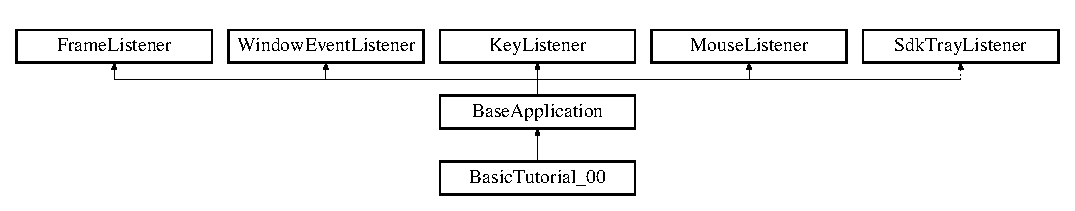
\includegraphics[height=2.382979cm]{class_base_application}
\end{center}
\end{figure}
\subsection*{Public Member Functions}
\begin{DoxyCompactItemize}
\item 
virtual void {\bfseries go} (void)\hypertarget{class_base_application_a8a14a65a29118dd75173aa68678a05e1}{}\label{class_base_application_a8a14a65a29118dd75173aa68678a05e1}

\end{DoxyCompactItemize}
\subsection*{Protected Member Functions}
\begin{DoxyCompactItemize}
\item 
virtual bool {\bfseries setup} ()\hypertarget{class_base_application_a5853d0e148cb85b0297a6885e1d33a89}{}\label{class_base_application_a5853d0e148cb85b0297a6885e1d33a89}

\item 
virtual bool {\bfseries configure} (void)\hypertarget{class_base_application_a62ed46f90e9f82cc810997647a2c587e}{}\label{class_base_application_a62ed46f90e9f82cc810997647a2c587e}

\item 
virtual void {\bfseries choose\+Scene\+Manager} (void)\hypertarget{class_base_application_ad5bc9655041e1849a4c13f444a3712bd}{}\label{class_base_application_ad5bc9655041e1849a4c13f444a3712bd}

\item 
virtual void {\bfseries create\+Camera} (void)\hypertarget{class_base_application_afa9d51527763cf9aee9cd4e1b1039d55}{}\label{class_base_application_afa9d51527763cf9aee9cd4e1b1039d55}

\item 
virtual void {\bfseries create\+Frame\+Listener} (void)\hypertarget{class_base_application_aff6fd9ff1ff0978cc68f19dd65be4778}{}\label{class_base_application_aff6fd9ff1ff0978cc68f19dd65be4778}

\item 
virtual void {\bfseries create\+Scene} (void)=0\hypertarget{class_base_application_aa97beeb4059b17d0ec22eae33286ec2d}{}\label{class_base_application_aa97beeb4059b17d0ec22eae33286ec2d}

\item 
virtual void {\bfseries destroy\+Scene} (void)\hypertarget{class_base_application_a365146059b25391fe400f5fdb94f011e}{}\label{class_base_application_a365146059b25391fe400f5fdb94f011e}

\item 
virtual void {\bfseries create\+Viewports} (void)\hypertarget{class_base_application_a1f8f6730cae6ec769d8730b1af48486e}{}\label{class_base_application_a1f8f6730cae6ec769d8730b1af48486e}

\item 
virtual void {\bfseries setup\+Resources} (void)\hypertarget{class_base_application_ae27301702f1e5de64619a39b1929f1f9}{}\label{class_base_application_ae27301702f1e5de64619a39b1929f1f9}

\item 
virtual void {\bfseries create\+Resource\+Listener} (void)\hypertarget{class_base_application_a9b77972f0f747a61e1f8ceba2ad47641}{}\label{class_base_application_a9b77972f0f747a61e1f8ceba2ad47641}

\item 
virtual void {\bfseries load\+Resources} (void)\hypertarget{class_base_application_aaeb764e637dd87601a81a80156659d88}{}\label{class_base_application_aaeb764e637dd87601a81a80156659d88}

\item 
virtual bool {\bfseries frame\+Rendering\+Queued} (const Ogre\+::\+Frame\+Event \&evt)\hypertarget{class_base_application_a03912a0f38b38fede7f08a2571e8fc56}{}\label{class_base_application_a03912a0f38b38fede7f08a2571e8fc56}

\item 
virtual bool {\bfseries key\+Pressed} (const O\+I\+S\+::\+Key\+Event \&arg)\hypertarget{class_base_application_acfa977f04e435f18018ece805c1277ec}{}\label{class_base_application_acfa977f04e435f18018ece805c1277ec}

\item 
virtual bool {\bfseries key\+Released} (const O\+I\+S\+::\+Key\+Event \&arg)\hypertarget{class_base_application_aba5c7c9dea7a0efc58b89310bae547e5}{}\label{class_base_application_aba5c7c9dea7a0efc58b89310bae547e5}

\item 
virtual bool {\bfseries mouse\+Moved} (const O\+I\+S\+::\+Mouse\+Event \&arg)\hypertarget{class_base_application_a126e59cb246b061e51eb6ce06a2ee8f4}{}\label{class_base_application_a126e59cb246b061e51eb6ce06a2ee8f4}

\item 
virtual bool {\bfseries mouse\+Pressed} (const O\+I\+S\+::\+Mouse\+Event \&arg, O\+I\+S\+::\+Mouse\+Button\+ID id)\hypertarget{class_base_application_a9255dfc1eabefd11c474ec45a6622504}{}\label{class_base_application_a9255dfc1eabefd11c474ec45a6622504}

\item 
virtual bool {\bfseries mouse\+Released} (const O\+I\+S\+::\+Mouse\+Event \&arg, O\+I\+S\+::\+Mouse\+Button\+ID id)\hypertarget{class_base_application_aa102c5859c14c0690c749994a446b53d}{}\label{class_base_application_aa102c5859c14c0690c749994a446b53d}

\item 
virtual void {\bfseries window\+Resized} (Ogre\+::\+Render\+Window $\ast$rw)\hypertarget{class_base_application_afacf8a797588592ef0abbad593f10cfa}{}\label{class_base_application_afacf8a797588592ef0abbad593f10cfa}

\item 
virtual void {\bfseries window\+Closed} (Ogre\+::\+Render\+Window $\ast$rw)\hypertarget{class_base_application_ae0e37ac54a31ff6e51d58c7654ad1b90}{}\label{class_base_application_ae0e37ac54a31ff6e51d58c7654ad1b90}

\end{DoxyCompactItemize}
\subsection*{Protected Attributes}
\begin{DoxyCompactItemize}
\item 
Ogre\+::\+Root $\ast$ {\bfseries m\+Root}\hypertarget{class_base_application_add84ba707dc6c57e6283f214b1274110}{}\label{class_base_application_add84ba707dc6c57e6283f214b1274110}

\item 
Ogre\+::\+Camera $\ast$ {\bfseries m\+Camera}\hypertarget{class_base_application_a3829c6b12afe911e97e6b4524b33a38b}{}\label{class_base_application_a3829c6b12afe911e97e6b4524b33a38b}

\item 
Ogre\+::\+Scene\+Manager $\ast$ {\bfseries m\+Scene\+Mgr}\hypertarget{class_base_application_a8a7684f4f9a57ed3089048ad1a913b2d}{}\label{class_base_application_a8a7684f4f9a57ed3089048ad1a913b2d}

\item 
Ogre\+::\+Render\+Window $\ast$ {\bfseries m\+Window}\hypertarget{class_base_application_ac5d8e9c81e036897bc82f81eff8c570f}{}\label{class_base_application_ac5d8e9c81e036897bc82f81eff8c570f}

\item 
Ogre\+::\+String {\bfseries m\+Resources\+Cfg}\hypertarget{class_base_application_a765e0df01c141a16df3178ab4f17afe6}{}\label{class_base_application_a765e0df01c141a16df3178ab4f17afe6}

\item 
Ogre\+::\+String {\bfseries m\+Plugins\+Cfg}\hypertarget{class_base_application_a04f2fe47fa164fd78d986dc0df70b7fb}{}\label{class_base_application_a04f2fe47fa164fd78d986dc0df70b7fb}

\item 
Ogre\+Bites\+::\+Sdk\+Tray\+Manager $\ast$ {\bfseries m\+Tray\+Mgr}\hypertarget{class_base_application_a7faa397f4f4861ee8c361a01e90b4416}{}\label{class_base_application_a7faa397f4f4861ee8c361a01e90b4416}

\item 
Ogre\+Bites\+::\+Sdk\+Camera\+Man $\ast$ {\bfseries m\+Camera\+Man}\hypertarget{class_base_application_a9ae38dea6316058549151fff66a91fcd}{}\label{class_base_application_a9ae38dea6316058549151fff66a91fcd}

\item 
Ogre\+Bites\+::\+Params\+Panel $\ast$ {\bfseries m\+Details\+Panel}\hypertarget{class_base_application_a6a11054ca61efdf558e0ff1b2de43a12}{}\label{class_base_application_a6a11054ca61efdf558e0ff1b2de43a12}

\item 
bool {\bfseries m\+Cursor\+Was\+Visible}\hypertarget{class_base_application_ac7e861799862cb645f1d78b170aef80d}{}\label{class_base_application_ac7e861799862cb645f1d78b170aef80d}

\item 
bool {\bfseries m\+Shut\+Down}\hypertarget{class_base_application_a755f26d3a9915aaf830750d877e39d86}{}\label{class_base_application_a755f26d3a9915aaf830750d877e39d86}

\item 
O\+I\+S\+::\+Input\+Manager $\ast$ {\bfseries m\+Input\+Manager}\hypertarget{class_base_application_abc9503c8462e225b5d0d55c952d9e4a9}{}\label{class_base_application_abc9503c8462e225b5d0d55c952d9e4a9}

\item 
O\+I\+S\+::\+Mouse $\ast$ {\bfseries m\+Mouse}\hypertarget{class_base_application_add9b97fbe64da2814d3af113bac58c43}{}\label{class_base_application_add9b97fbe64da2814d3af113bac58c43}

\item 
O\+I\+S\+::\+Keyboard $\ast$ {\bfseries m\+Keyboard}\hypertarget{class_base_application_a9d6e19cf50c47379fbaae55bff28079c}{}\label{class_base_application_a9d6e19cf50c47379fbaae55bff28079c}

\end{DoxyCompactItemize}


\subsection{Detailed Description}
base class for application 

The documentation for this class was generated from the following files\+:\begin{DoxyCompactItemize}
\item 
programs/\+Obstacle/include/Base\+Application.\+h\item 
programs/\+Obstacle/source/Base\+Application.\+cpp\end{DoxyCompactItemize}

\hypertarget{class_basic_tutorial__00}{}\section{Basic\+Tutorial\+\_\+00 Class Reference}
\label{class_basic_tutorial__00}\index{Basic\+Tutorial\+\_\+00@{Basic\+Tutorial\+\_\+00}}


main class for the application  




{\ttfamily \#include $<$Tutorial\+Application.\+h$>$}

Inheritance diagram for Basic\+Tutorial\+\_\+00\+:\begin{figure}[H]
\begin{center}
\leavevmode
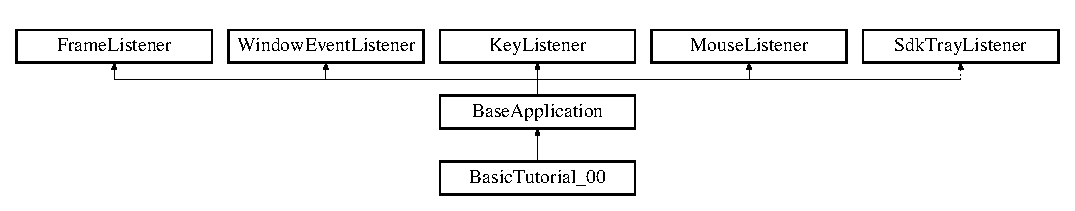
\includegraphics[height=2.382979cm]{class_basic_tutorial__00}
\end{center}
\end{figure}
\subsection*{Public Member Functions}
\begin{DoxyCompactItemize}
\item 
\hyperlink{class_basic_tutorial__00_a6b55068822076b28e7819b1878e95684}{Basic\+Tutorial\+\_\+00} (void)\hypertarget{class_basic_tutorial__00_a6b55068822076b28e7819b1878e95684}{}\label{class_basic_tutorial__00_a6b55068822076b28e7819b1878e95684}

\begin{DoxyCompactList}\small\item\em constructor \end{DoxyCompactList}\item 
\hyperlink{class_basic_tutorial__00_a9df0243c6c09c5e3d182dc242b90a90b}{$\sim$\+Basic\+Tutorial\+\_\+00} (void)\hypertarget{class_basic_tutorial__00_a9df0243c6c09c5e3d182dc242b90a90b}{}\label{class_basic_tutorial__00_a9df0243c6c09c5e3d182dc242b90a90b}

\begin{DoxyCompactList}\small\item\em destructor \end{DoxyCompactList}\item 
virtual void \hyperlink{class_basic_tutorial__00_a15a3d4673724ec99077ce992f996a550}{create\+Scene} (void)\hypertarget{class_basic_tutorial__00_a15a3d4673724ec99077ce992f996a550}{}\label{class_basic_tutorial__00_a15a3d4673724ec99077ce992f996a550}

\begin{DoxyCompactList}\small\item\em create the scene \end{DoxyCompactList}\item 
virtual bool \hyperlink{class_basic_tutorial__00_a74d6b3b32ddf53aeb178540617b86045}{is\+Started} ()\hypertarget{class_basic_tutorial__00_a74d6b3b32ddf53aeb178540617b86045}{}\label{class_basic_tutorial__00_a74d6b3b32ddf53aeb178540617b86045}

\begin{DoxyCompactList}\small\item\em is game started? \end{DoxyCompactList}\item 
virtual bool \hyperlink{class_basic_tutorial__00_a58ef600ec65f7f04dc5520b9b9185f5b}{is\+Paused} ()\hypertarget{class_basic_tutorial__00_a58ef600ec65f7f04dc5520b9b9185f5b}{}\label{class_basic_tutorial__00_a58ef600ec65f7f04dc5520b9b9185f5b}

\begin{DoxyCompactList}\small\item\em is game paused? \end{DoxyCompactList}\item 
virtual bool \hyperlink{class_basic_tutorial__00_a5f4f1c065645bcbb9e0312e4a06e3c8e}{is\+Overed} ()\hypertarget{class_basic_tutorial__00_a5f4f1c065645bcbb9e0312e4a06e3c8e}{}\label{class_basic_tutorial__00_a5f4f1c065645bcbb9e0312e4a06e3c8e}

\begin{DoxyCompactList}\small\item\em is game overed? \end{DoxyCompactList}\item 
virtual \hyperlink{class_n_c_t_u_1_1_player_obstacle}{N\+C\+T\+U\+::\+Player\+Obstacle} $\ast$ \hyperlink{class_basic_tutorial__00_a556b34103cda909d74561bfd779d7c89}{get\+Player} ()\hypertarget{class_basic_tutorial__00_a556b34103cda909d74561bfd779d7c89}{}\label{class_basic_tutorial__00_a556b34103cda909d74561bfd779d7c89}

\begin{DoxyCompactList}\small\item\em get the player obstacle \end{DoxyCompactList}\item 
virtual bool \hyperlink{class_basic_tutorial__00_adc1a0b32d78b1980b3ee51a1b1e1e69b}{key\+Pressed} (const O\+I\+S\+::\+Key\+Event \&arg)\hypertarget{class_basic_tutorial__00_adc1a0b32d78b1980b3ee51a1b1e1e69b}{}\label{class_basic_tutorial__00_adc1a0b32d78b1980b3ee51a1b1e1e69b}

\begin{DoxyCompactList}\small\item\em O\+IS -\/ key\+Pressed. \end{DoxyCompactList}\item 
virtual bool \hyperlink{class_basic_tutorial__00_aacca7a0a2a5a0e0d007b9c6c30b4941b}{key\+Released} (const O\+I\+S\+::\+Key\+Event \&arg)\hypertarget{class_basic_tutorial__00_aacca7a0a2a5a0e0d007b9c6c30b4941b}{}\label{class_basic_tutorial__00_aacca7a0a2a5a0e0d007b9c6c30b4941b}

\begin{DoxyCompactList}\small\item\em O\+IS -\/ key\+Released. \end{DoxyCompactList}\item 
virtual bool \hyperlink{class_basic_tutorial__00_a5b9bd30851c38fa6c2fa102f30e9629a}{mouse\+Moved} (const O\+I\+S\+::\+Mouse\+Event \&arg)\hypertarget{class_basic_tutorial__00_a5b9bd30851c38fa6c2fa102f30e9629a}{}\label{class_basic_tutorial__00_a5b9bd30851c38fa6c2fa102f30e9629a}

\begin{DoxyCompactList}\small\item\em O\+IS -\/ mouse\+Moved. \end{DoxyCompactList}\item 
virtual bool \hyperlink{class_basic_tutorial__00_af0e5dec72c58e157c2a63ffa5fd8c7c7}{mouse\+Pressed} (const O\+I\+S\+::\+Mouse\+Event \&arg, O\+I\+S\+::\+Mouse\+Button\+ID id)\hypertarget{class_basic_tutorial__00_af0e5dec72c58e157c2a63ffa5fd8c7c7}{}\label{class_basic_tutorial__00_af0e5dec72c58e157c2a63ffa5fd8c7c7}

\begin{DoxyCompactList}\small\item\em O\+IS -\/ mouse\+Pressed. \end{DoxyCompactList}\item 
virtual bool \hyperlink{class_basic_tutorial__00_aeb28d7b68dcaf536f513e25afb6947d7}{mouse\+Released} (const O\+I\+S\+::\+Mouse\+Event \&arg, O\+I\+S\+::\+Mouse\+Button\+ID id)\hypertarget{class_basic_tutorial__00_aeb28d7b68dcaf536f513e25afb6947d7}{}\label{class_basic_tutorial__00_aeb28d7b68dcaf536f513e25afb6947d7}

\begin{DoxyCompactList}\small\item\em O\+IS -\/ mouse\+Released. \end{DoxyCompactList}\item 
virtual void \hyperlink{class_basic_tutorial__00_a875932b8b12f508f432cba994934ff8c}{start\+Game} ()\hypertarget{class_basic_tutorial__00_a875932b8b12f508f432cba994934ff8c}{}\label{class_basic_tutorial__00_a875932b8b12f508f432cba994934ff8c}

\begin{DoxyCompactList}\small\item\em start the game \end{DoxyCompactList}\item 
virtual void \hyperlink{class_basic_tutorial__00_a98d19aa5e1a903e86e5a900f7b2d768b}{exit\+Game} ()\hypertarget{class_basic_tutorial__00_a98d19aa5e1a903e86e5a900f7b2d768b}{}\label{class_basic_tutorial__00_a98d19aa5e1a903e86e5a900f7b2d768b}

\begin{DoxyCompactList}\small\item\em exit game \end{DoxyCompactList}\item 
virtual void \hyperlink{class_basic_tutorial__00_a46299119fe4c936154cd8c5d346a3a5c}{pause\+Game} ()\hypertarget{class_basic_tutorial__00_a46299119fe4c936154cd8c5d346a3a5c}{}\label{class_basic_tutorial__00_a46299119fe4c936154cd8c5d346a3a5c}

\begin{DoxyCompactList}\small\item\em pause game \end{DoxyCompactList}\item 
virtual void \hyperlink{class_basic_tutorial__00_a1783c0d4e754ed8fbd309518599d68f4}{resume\+Game} ()\hypertarget{class_basic_tutorial__00_a1783c0d4e754ed8fbd309518599d68f4}{}\label{class_basic_tutorial__00_a1783c0d4e754ed8fbd309518599d68f4}

\begin{DoxyCompactList}\small\item\em resume game \end{DoxyCompactList}\item 
virtual void \hyperlink{class_basic_tutorial__00_a90b8afe85502db0ca9d857427f29a78f}{back\+To\+Main\+Menu} ()\hypertarget{class_basic_tutorial__00_a90b8afe85502db0ca9d857427f29a78f}{}\label{class_basic_tutorial__00_a90b8afe85502db0ca9d857427f29a78f}

\begin{DoxyCompactList}\small\item\em back to main menu \end{DoxyCompactList}\item 
virtual void \hyperlink{class_basic_tutorial__00_a2a43461909048d1a9aa5ec25650e5933}{reset\+Game} ()\hypertarget{class_basic_tutorial__00_a2a43461909048d1a9aa5ec25650e5933}{}\label{class_basic_tutorial__00_a2a43461909048d1a9aa5ec25650e5933}

\begin{DoxyCompactList}\small\item\em reset game to starting state \end{DoxyCompactList}\item 
virtual void \hyperlink{class_basic_tutorial__00_a41d62aea8f1991df4e3e14db5f4bb4f3}{enter\+Level\+Menu} ()\hypertarget{class_basic_tutorial__00_a41d62aea8f1991df4e3e14db5f4bb4f3}{}\label{class_basic_tutorial__00_a41d62aea8f1991df4e3e14db5f4bb4f3}

\begin{DoxyCompactList}\small\item\em go to level selection menu \end{DoxyCompactList}\item 
virtual void \hyperlink{class_basic_tutorial__00_a6a967f56136eae966364b10a9e58d88a}{exit\+Level\+Menu} ()\hypertarget{class_basic_tutorial__00_a6a967f56136eae966364b10a9e58d88a}{}\label{class_basic_tutorial__00_a6a967f56136eae966364b10a9e58d88a}

\begin{DoxyCompactList}\small\item\em exit level selection menu \end{DoxyCompactList}\item 
void \hyperlink{class_basic_tutorial__00_a5e0cbb9bab080bed9aa7d1919bea36dc}{refresh\+Score} ()\hypertarget{class_basic_tutorial__00_a5e0cbb9bab080bed9aa7d1919bea36dc}{}\label{class_basic_tutorial__00_a5e0cbb9bab080bed9aa7d1919bea36dc}

\begin{DoxyCompactList}\small\item\em refresh the score \end{DoxyCompactList}\item 
int \& \hyperlink{class_basic_tutorial__00_a376cbc51afc862822eb4d6a4c3371cb1}{score} ()\hypertarget{class_basic_tutorial__00_a376cbc51afc862822eb4d6a4c3371cb1}{}\label{class_basic_tutorial__00_a376cbc51afc862822eb4d6a4c3371cb1}

\begin{DoxyCompactList}\small\item\em get current score \end{DoxyCompactList}\item 
void \hyperlink{class_basic_tutorial__00_a478be738fa4414c86c4bb5b1955853ea}{change\+Score} (int val)\hypertarget{class_basic_tutorial__00_a478be738fa4414c86c4bb5b1955853ea}{}\label{class_basic_tutorial__00_a478be738fa4414c86c4bb5b1955853ea}

\begin{DoxyCompactList}\small\item\em change score \end{DoxyCompactList}\item 
virtual const String \& \hyperlink{class_basic_tutorial__00_aa230d468c40ca1efe0cb8832c6308609}{get\+Current\+Level\+Name} () const \hypertarget{class_basic_tutorial__00_aa230d468c40ca1efe0cb8832c6308609}{}\label{class_basic_tutorial__00_aa230d468c40ca1efe0cb8832c6308609}

\begin{DoxyCompactList}\small\item\em get current level name \end{DoxyCompactList}\item 
virtual void \hyperlink{class_basic_tutorial__00_a20579e2759d963371d6598bbacf8a631}{set\+Current\+Level\+Name} (const String \&)\hypertarget{class_basic_tutorial__00_a20579e2759d963371d6598bbacf8a631}{}\label{class_basic_tutorial__00_a20579e2759d963371d6598bbacf8a631}

\begin{DoxyCompactList}\small\item\em set current level name \end{DoxyCompactList}\item 
void \hyperlink{class_basic_tutorial__00_a5e5d38d07a0e01b1f7bf4771b01e276e}{on\+Pickup\+Get} ()\hypertarget{class_basic_tutorial__00_a5e5d38d07a0e01b1f7bf4771b01e276e}{}\label{class_basic_tutorial__00_a5e5d38d07a0e01b1f7bf4771b01e276e}

\begin{DoxyCompactList}\small\item\em process when get a pickup object \end{DoxyCompactList}\end{DoxyCompactItemize}
\subsection*{Protected Member Functions}
\begin{DoxyCompactItemize}
\item 
virtual void \hyperlink{class_basic_tutorial__00_a1bf709417d654dffc2ea10987412b912}{create\+Camera} (void)\hypertarget{class_basic_tutorial__00_a1bf709417d654dffc2ea10987412b912}{}\label{class_basic_tutorial__00_a1bf709417d654dffc2ea10987412b912}

\begin{DoxyCompactList}\small\item\em create camera \end{DoxyCompactList}\item 
virtual bool \hyperlink{class_basic_tutorial__00_aa02aec0fcd3211e00bcb6d6d259a1ec6}{frame\+Started} (const Frame\+Event \&evt)\hypertarget{class_basic_tutorial__00_aa02aec0fcd3211e00bcb6d6d259a1ec6}{}\label{class_basic_tutorial__00_aa02aec0fcd3211e00bcb6d6d259a1ec6}

\begin{DoxyCompactList}\small\item\em process for frame\+Started \end{DoxyCompactList}\item 
virtual void \hyperlink{class_basic_tutorial__00_ace40938ce3e816495bdb46743db100d6}{update\+Basic} (const Frame\+Event \&evt)\hypertarget{class_basic_tutorial__00_ace40938ce3e816495bdb46743db100d6}{}\label{class_basic_tutorial__00_ace40938ce3e816495bdb46743db100d6}

\begin{DoxyCompactList}\small\item\em update basic game functionallity \end{DoxyCompactList}\item 
virtual void \hyperlink{class_basic_tutorial__00_a8c9934b2cef28309cd70752e72bebc1d}{update\+Playing\+Game} (const Frame\+Event \&evt)\hypertarget{class_basic_tutorial__00_a8c9934b2cef28309cd70752e72bebc1d}{}\label{class_basic_tutorial__00_a8c9934b2cef28309cd70752e72bebc1d}

\begin{DoxyCompactList}\small\item\em update routine for playing game \end{DoxyCompactList}\item 
virtual void \hyperlink{class_basic_tutorial__00_a65d00df4d4b3cfab41e7779a5830c8a3}{update\+Paused\+Game} (const Frame\+Event \&evt)\hypertarget{class_basic_tutorial__00_a65d00df4d4b3cfab41e7779a5830c8a3}{}\label{class_basic_tutorial__00_a65d00df4d4b3cfab41e7779a5830c8a3}

\begin{DoxyCompactList}\small\item\em update routine for paused game \end{DoxyCompactList}\item 
virtual void \hyperlink{class_basic_tutorial__00_a6ca5eb34b732ed3621f0b15cfa726ba8}{process\+Input\+Basic} (const Frame\+Event \&evt)\hypertarget{class_basic_tutorial__00_a6ca5eb34b732ed3621f0b15cfa726ba8}{}\label{class_basic_tutorial__00_a6ca5eb34b732ed3621f0b15cfa726ba8}

\begin{DoxyCompactList}\small\item\em process input event for all cases \end{DoxyCompactList}\item 
virtual void \hyperlink{class_basic_tutorial__00_a369c001eb86a792d15b3d1aefdd7b030}{process\+Input\+Playing\+Game} (const Frame\+Event \&evt)\hypertarget{class_basic_tutorial__00_a369c001eb86a792d15b3d1aefdd7b030}{}\label{class_basic_tutorial__00_a369c001eb86a792d15b3d1aefdd7b030}

\begin{DoxyCompactList}\small\item\em process extra input event for playing game \end{DoxyCompactList}\item 
virtual void \hyperlink{class_basic_tutorial__00_a56a6c761ca0a639a11f1634e5f37a300}{process\+Input\+Paused\+Game} (const Frame\+Event \&evt)\hypertarget{class_basic_tutorial__00_a56a6c761ca0a639a11f1634e5f37a300}{}\label{class_basic_tutorial__00_a56a6c761ca0a639a11f1634e5f37a300}

\begin{DoxyCompactList}\small\item\em process extra input evnet for paused game \end{DoxyCompactList}\item 
virtual Real \hyperlink{class_basic_tutorial__00_abf7135bae86a71ec26344f1226bc70c0}{speed\+Adjustment} (const Vector3 \&old, const Vector3 \&go)\hypertarget{class_basic_tutorial__00_abf7135bae86a71ec26344f1226bc70c0}{}\label{class_basic_tutorial__00_abf7135bae86a71ec26344f1226bc70c0}

\begin{DoxyCompactList}\small\item\em adjust the moving speed (manual control only) \end{DoxyCompactList}\item 
virtual void \hyperlink{class_basic_tutorial__00_a013e1d3a955971b0b9cbdd0d34f6efd7}{check\+Collision} (const Frame\+Event \&evt)\hypertarget{class_basic_tutorial__00_a013e1d3a955971b0b9cbdd0d34f6efd7}{}\label{class_basic_tutorial__00_a013e1d3a955971b0b9cbdd0d34f6efd7}

\begin{DoxyCompactList}\small\item\em check collision \end{DoxyCompactList}\item 
virtual void \hyperlink{class_basic_tutorial__00_ab5e701d1142693b4404ce672444e0f14}{update\+Light\+Position} (const Frame\+Event \&evt)\hypertarget{class_basic_tutorial__00_ab5e701d1142693b4404ce672444e0f14}{}\label{class_basic_tutorial__00_ab5e701d1142693b4404ce672444e0f14}

\begin{DoxyCompactList}\small\item\em update the light position \end{DoxyCompactList}\item 
virtual void \hyperlink{class_basic_tutorial__00_abfe0cf98461d76fc3e9be5b417f0d94f}{equalize\+Speed} (const Frame\+Event \&evt)\hypertarget{class_basic_tutorial__00_abfe0cf98461d76fc3e9be5b417f0d94f}{}\label{class_basic_tutorial__00_abfe0cf98461d76fc3e9be5b417f0d94f}

\begin{DoxyCompactList}\small\item\em equalize the moving speed of player \end{DoxyCompactList}\item 
virtual void \hyperlink{class_basic_tutorial__00_aea14b000cfa10783029c299420220cfe}{fix\+Orientation} (const Frame\+Event \&evt)\hypertarget{class_basic_tutorial__00_aea14b000cfa10783029c299420220cfe}{}\label{class_basic_tutorial__00_aea14b000cfa10783029c299420220cfe}

\begin{DoxyCompactList}\small\item\em fix the orientation of player \end{DoxyCompactList}\item 
virtual Vector3 \hyperlink{class_basic_tutorial__00_a5a67f94bedcf0049a718b5c325f33c42}{get\+Front\+Direction} ()\hypertarget{class_basic_tutorial__00_a5a67f94bedcf0049a718b5c325f33c42}{}\label{class_basic_tutorial__00_a5a67f94bedcf0049a718b5c325f33c42}

\begin{DoxyCompactList}\small\item\em get the front direction \end{DoxyCompactList}\item 
void \hyperlink{class_basic_tutorial__00_a6f332c7915c0419f355cd901a69999b1}{load\+Level\+From\+Scene} (const String \&scene\+Name)\hypertarget{class_basic_tutorial__00_a6f332c7915c0419f355cd901a69999b1}{}\label{class_basic_tutorial__00_a6f332c7915c0419f355cd901a69999b1}

\begin{DoxyCompactList}\small\item\em load scene from scene name \end{DoxyCompactList}\item 
void \hyperlink{class_basic_tutorial__00_abaf653f7f04698804387dce117bbec10}{on\+Lose\+Game} ()\hypertarget{class_basic_tutorial__00_abaf653f7f04698804387dce117bbec10}{}\label{class_basic_tutorial__00_abaf653f7f04698804387dce117bbec10}

\begin{DoxyCompactList}\small\item\em process when player lose \end{DoxyCompactList}\end{DoxyCompactItemize}
\subsection*{Protected Attributes}
\begin{DoxyCompactItemize}
\item 
\hyperlink{class_n_c_t_u_1_1_obstacle_manager}{N\+C\+T\+U\+::\+Obstacle\+Manager} $\ast$ \hyperlink{class_basic_tutorial__00_a67b7798cecaa2ece062c7d1117a95d82}{m\+Obstacle\+Mgr}\hypertarget{class_basic_tutorial__00_a67b7798cecaa2ece062c7d1117a95d82}{}\label{class_basic_tutorial__00_a67b7798cecaa2ece062c7d1117a95d82}

\begin{DoxyCompactList}\small\item\em pointer to the obstacle manager \end{DoxyCompactList}\item 
Vector3 \hyperlink{class_basic_tutorial__00_a02f256951f4c99412b7bfefc70a48df9}{m\+Init\+Velocity}\hypertarget{class_basic_tutorial__00_a02f256951f4c99412b7bfefc70a48df9}{}\label{class_basic_tutorial__00_a02f256951f4c99412b7bfefc70a48df9}

\begin{DoxyCompactList}\small\item\em initial velocity for player \end{DoxyCompactList}\item 
Vector3 \hyperlink{class_basic_tutorial__00_a9ca4f04638d71851d093612b50c829ff}{m\+Init\+Position}\hypertarget{class_basic_tutorial__00_a9ca4f04638d71851d093612b50c829ff}{}\label{class_basic_tutorial__00_a9ca4f04638d71851d093612b50c829ff}

\begin{DoxyCompactList}\small\item\em initial position for player \end{DoxyCompactList}\item 
Quaternion \hyperlink{class_basic_tutorial__00_a019ffab159b6fe6807be9ee7cedc43bd}{m\+Init\+Orientation}\hypertarget{class_basic_tutorial__00_a019ffab159b6fe6807be9ee7cedc43bd}{}\label{class_basic_tutorial__00_a019ffab159b6fe6807be9ee7cedc43bd}

\begin{DoxyCompactList}\small\item\em inital orientation for player \end{DoxyCompactList}\item 
\hyperlink{class_n_c_t_u_1_1_player_obstacle}{N\+C\+T\+U\+::\+Player\+Obstacle} $\ast$ \hyperlink{class_basic_tutorial__00_a54bd813d5463fdd7823feeb41f7c3e74}{m\+Player\+Obstacle}\hypertarget{class_basic_tutorial__00_a54bd813d5463fdd7823feeb41f7c3e74}{}\label{class_basic_tutorial__00_a54bd813d5463fdd7823feeb41f7c3e74}

\begin{DoxyCompactList}\small\item\em pointer to the player obstacle \end{DoxyCompactList}\item 
\hyperlink{class_n_c_t_u_1_1_floor_obstacle}{N\+C\+T\+U\+::\+Floor\+Obstacle} $\ast$ \hyperlink{class_basic_tutorial__00_adced816949c00a34b016e469494f882c}{m\+Floor}\hypertarget{class_basic_tutorial__00_adced816949c00a34b016e469494f882c}{}\label{class_basic_tutorial__00_adced816949c00a34b016e469494f882c}

\begin{DoxyCompactList}\small\item\em pointer to the floor obstacle \end{DoxyCompactList}\item 
Light $\ast$ \hyperlink{class_basic_tutorial__00_a8bcbfe5308efb338acbf1250fdb69812}{m\+Light}\hypertarget{class_basic_tutorial__00_a8bcbfe5308efb338acbf1250fdb69812}{}\label{class_basic_tutorial__00_a8bcbfe5308efb338acbf1250fdb69812}

\begin{DoxyCompactList}\small\item\em pointer to the light \end{DoxyCompactList}\item 
\hyperlink{class_key_board_handler}{Key\+Board\+Handler} $\ast$ \hyperlink{class_basic_tutorial__00_a1b3c9aa12e011c9dc1cdb7280de71c56}{keyboardhandler}\hypertarget{class_basic_tutorial__00_a1b3c9aa12e011c9dc1cdb7280de71c56}{}\label{class_basic_tutorial__00_a1b3c9aa12e011c9dc1cdb7280de71c56}

\begin{DoxyCompactList}\small\item\em pointer to the keyboard handler \end{DoxyCompactList}\item 
bool \hyperlink{class_basic_tutorial__00_ae8b7440d91e7b4fe53f382ae41ff4d3f}{m\+Enable\+Collision}\hypertarget{class_basic_tutorial__00_ae8b7440d91e7b4fe53f382ae41ff4d3f}{}\label{class_basic_tutorial__00_ae8b7440d91e7b4fe53f382ae41ff4d3f}

\begin{DoxyCompactList}\small\item\em is the collision enabled? \end{DoxyCompactList}\item 
bool \hyperlink{class_basic_tutorial__00_af8c21ccb0a881cfb6c701890942e9c3a}{m\+Enable\+Free\+Mode}\hypertarget{class_basic_tutorial__00_af8c21ccb0a881cfb6c701890942e9c3a}{}\label{class_basic_tutorial__00_af8c21ccb0a881cfb6c701890942e9c3a}

\begin{DoxyCompactList}\small\item\em is the free view mode enabled? \end{DoxyCompactList}\item 
bool \hyperlink{class_basic_tutorial__00_a2d0fb4ce35996bb067ba56552318077c}{m\+Disable\+Lose}\hypertarget{class_basic_tutorial__00_a2d0fb4ce35996bb067ba56552318077c}{}\label{class_basic_tutorial__00_a2d0fb4ce35996bb067ba56552318077c}

\begin{DoxyCompactList}\small\item\em is the lose disabled? \end{DoxyCompactList}\item 
bool \hyperlink{class_basic_tutorial__00_a10b877ea0ad047d5b0032b8b31049f79}{m\+Game\+Started}\hypertarget{class_basic_tutorial__00_a10b877ea0ad047d5b0032b8b31049f79}{}\label{class_basic_tutorial__00_a10b877ea0ad047d5b0032b8b31049f79}

\begin{DoxyCompactList}\small\item\em is game started? \end{DoxyCompactList}\item 
bool \hyperlink{class_basic_tutorial__00_a194d7e653dfce68da37b9bcfb9eccfbc}{m\+Game\+Paused}\hypertarget{class_basic_tutorial__00_a194d7e653dfce68da37b9bcfb9eccfbc}{}\label{class_basic_tutorial__00_a194d7e653dfce68da37b9bcfb9eccfbc}

\begin{DoxyCompactList}\small\item\em is game paused? \end{DoxyCompactList}\item 
bool \hyperlink{class_basic_tutorial__00_adbb03178ebf7a7a35681f0f6e080f32a}{m\+Game\+Overed}\hypertarget{class_basic_tutorial__00_adbb03178ebf7a7a35681f0f6e080f32a}{}\label{class_basic_tutorial__00_adbb03178ebf7a7a35681f0f6e080f32a}

\begin{DoxyCompactList}\small\item\em is game overed? \end{DoxyCompactList}\item 
Real \hyperlink{class_basic_tutorial__00_a09635c00def305e11a1041ea639b738f}{m\+Speed\+Rate}\hypertarget{class_basic_tutorial__00_a09635c00def305e11a1041ea639b738f}{}\label{class_basic_tutorial__00_a09635c00def305e11a1041ea639b738f}

\begin{DoxyCompactList}\small\item\em the speed rate for player \end{DoxyCompactList}\item 
Real \hyperlink{class_basic_tutorial__00_a30c30dbab84babfc29fb95c026af04ac}{m\+Bullet\+Life\+Time}\hypertarget{class_basic_tutorial__00_a30c30dbab84babfc29fb95c026af04ac}{}\label{class_basic_tutorial__00_a30c30dbab84babfc29fb95c026af04ac}

\begin{DoxyCompactList}\small\item\em bullet lift time \end{DoxyCompactList}\item 
Real \hyperlink{class_basic_tutorial__00_a2ba5a47eb3dfab049aafafcee0620fac}{m\+Bullet\+Speed\+Factor}\hypertarget{class_basic_tutorial__00_a2ba5a47eb3dfab049aafafcee0620fac}{}\label{class_basic_tutorial__00_a2ba5a47eb3dfab049aafafcee0620fac}

\begin{DoxyCompactList}\small\item\em bullet speed factor \end{DoxyCompactList}\item 
Real \hyperlink{class_basic_tutorial__00_a152a7b0fc73894847589ebb4faf28067}{m\+Air\+Jump\+Speed}\hypertarget{class_basic_tutorial__00_a152a7b0fc73894847589ebb4faf28067}{}\label{class_basic_tutorial__00_a152a7b0fc73894847589ebb4faf28067}

\begin{DoxyCompactList}\small\item\em player air jump speed (currently not used) \end{DoxyCompactList}\item 
int \hyperlink{class_basic_tutorial__00_ab655d56fb51268b3edfa38059be04fc3}{m\+Air\+Jump\+Left}\hypertarget{class_basic_tutorial__00_ab655d56fb51268b3edfa38059be04fc3}{}\label{class_basic_tutorial__00_ab655d56fb51268b3edfa38059be04fc3}

\begin{DoxyCompactList}\small\item\em air jump time left \end{DoxyCompactList}\item 
int \hyperlink{class_basic_tutorial__00_a58590c7cf95e3a9d38dbfb4e25c9068f}{m\+Air\+Jump\+Max}\hypertarget{class_basic_tutorial__00_a58590c7cf95e3a9d38dbfb4e25c9068f}{}\label{class_basic_tutorial__00_a58590c7cf95e3a9d38dbfb4e25c9068f}

\begin{DoxyCompactList}\small\item\em max air jmup time \end{DoxyCompactList}\item 
int \hyperlink{class_basic_tutorial__00_ae5a09bb19034dd70b3dbdd85e0e9e97c}{m\+Score}\hypertarget{class_basic_tutorial__00_ae5a09bb19034dd70b3dbdd85e0e9e97c}{}\label{class_basic_tutorial__00_ae5a09bb19034dd70b3dbdd85e0e9e97c}

\begin{DoxyCompactList}\small\item\em score \end{DoxyCompactList}\item 
Real \hyperlink{class_basic_tutorial__00_ac7a3601eca27a49db62b38d6865c0696}{m\+Time\+Score\+Temp}\hypertarget{class_basic_tutorial__00_ac7a3601eca27a49db62b38d6865c0696}{}\label{class_basic_tutorial__00_ac7a3601eca27a49db62b38d6865c0696}

\begin{DoxyCompactList}\small\item\em score temp variable \end{DoxyCompactList}\item 
double \hyperlink{class_basic_tutorial__00_a916f7aa61c77bb9e55e05d45213e1eca}{m\+Time\+Elapsed}\hypertarget{class_basic_tutorial__00_a916f7aa61c77bb9e55e05d45213e1eca}{}\label{class_basic_tutorial__00_a916f7aa61c77bb9e55e05d45213e1eca}

\begin{DoxyCompactList}\small\item\em time elapsed \end{DoxyCompactList}\item 
Real \hyperlink{class_basic_tutorial__00_a3846577b96d2ce7edfa095ee717a6c30}{m\+Pause\+Time\+Interval}\hypertarget{class_basic_tutorial__00_a3846577b96d2ce7edfa095ee717a6c30}{}\label{class_basic_tutorial__00_a3846577b96d2ce7edfa095ee717a6c30}

\begin{DoxyCompactList}\small\item\em pause time interval \end{DoxyCompactList}\item 
Real \hyperlink{class_basic_tutorial__00_a1ce08f37c4d14d4f074844bcc3c6b062}{m\+Pause\+Time\+Interval\+Max}\hypertarget{class_basic_tutorial__00_a1ce08f37c4d14d4f074844bcc3c6b062}{}\label{class_basic_tutorial__00_a1ce08f37c4d14d4f074844bcc3c6b062}

\begin{DoxyCompactList}\small\item\em max pause time interval \end{DoxyCompactList}\item 
Vector3 \hyperlink{class_basic_tutorial__00_a12a1faab9b1d6fbc18124c84e76031f4}{m\+Light\+Offset}\hypertarget{class_basic_tutorial__00_a12a1faab9b1d6fbc18124c84e76031f4}{}\label{class_basic_tutorial__00_a12a1faab9b1d6fbc18124c84e76031f4}

\begin{DoxyCompactList}\small\item\em light offset \end{DoxyCompactList}\item 
int \hyperlink{class_basic_tutorial__00_aa3da4d61ee5303a5cd3e98cb1b717372}{current\+Direction}\hypertarget{class_basic_tutorial__00_aa3da4d61ee5303a5cd3e98cb1b717372}{}\label{class_basic_tutorial__00_aa3da4d61ee5303a5cd3e98cb1b717372}

\begin{DoxyCompactList}\small\item\em current direction \end{DoxyCompactList}\item 
Vector3 \hyperlink{class_basic_tutorial__00_a2d535104287a3a67b670c61bb176dfdd}{m\+Direction\+Vectors} \mbox{[}4\mbox{]}\hypertarget{class_basic_tutorial__00_a2d535104287a3a67b670c61bb176dfdd}{}\label{class_basic_tutorial__00_a2d535104287a3a67b670c61bb176dfdd}

\begin{DoxyCompactList}\small\item\em direction vectors \end{DoxyCompactList}\item 
\hyperlink{class_ogre_1_1_dot_scene_loader}{Dot\+Scene\+Loader} \hyperlink{class_basic_tutorial__00_abce6706ed27450e6595c46ed3a679541}{m\+Dot\+Scene}\hypertarget{class_basic_tutorial__00_abce6706ed27450e6595c46ed3a679541}{}\label{class_basic_tutorial__00_abce6706ed27450e6595c46ed3a679541}

\begin{DoxyCompactList}\small\item\em pointer to dot\+Scene loader \end{DoxyCompactList}\item 
\hyperlink{class_n_c_t_u_1_1_g_u_i_manager}{N\+C\+T\+U\+::\+G\+U\+I\+Manager} $\ast$ \hyperlink{class_basic_tutorial__00_a2cf169aa305a3fed9f08acb778f1c029}{m\+G\+UI}\hypertarget{class_basic_tutorial__00_a2cf169aa305a3fed9f08acb778f1c029}{}\label{class_basic_tutorial__00_a2cf169aa305a3fed9f08acb778f1c029}

\begin{DoxyCompactList}\small\item\em pointer to G\+UI manager \end{DoxyCompactList}\item 
\hyperlink{class_n_c_t_u_camera}{N\+C\+T\+U\+Camera} $\ast$ \hyperlink{class_basic_tutorial__00_a06bc4644751657e95cf03f6554257658}{m\+Camera\+Ctrl}\hypertarget{class_basic_tutorial__00_a06bc4644751657e95cf03f6554257658}{}\label{class_basic_tutorial__00_a06bc4644751657e95cf03f6554257658}

\begin{DoxyCompactList}\small\item\em pointer to camera controller \end{DoxyCompactList}\item 
String \hyperlink{class_basic_tutorial__00_aa2fcff6c794db576838456e6b8626524}{m\+Current\+Level\+Name}\hypertarget{class_basic_tutorial__00_aa2fcff6c794db576838456e6b8626524}{}\label{class_basic_tutorial__00_aa2fcff6c794db576838456e6b8626524}

\begin{DoxyCompactList}\small\item\em current level name \end{DoxyCompactList}\item 
String \hyperlink{class_basic_tutorial__00_ab0503757c829a4a80e7d235840a43e7b}{m\+Current\+B\+GM}\hypertarget{class_basic_tutorial__00_ab0503757c829a4a80e7d235840a43e7b}{}\label{class_basic_tutorial__00_ab0503757c829a4a80e7d235840a43e7b}

\begin{DoxyCompactList}\small\item\em current bgm \end{DoxyCompactList}\end{DoxyCompactItemize}


\subsection{Detailed Description}
main class for the application 

The documentation for this class was generated from the following files\+:\begin{DoxyCompactItemize}
\item 
programs/\+Obstacle/include/Tutorial\+Application.\+h\item 
programs/\+Obstacle/source/Tutorial\+Application.\+cpp\end{DoxyCompactItemize}

\hypertarget{struct_n_c_t_u_1_1_bullet_contact_result_callback}{}\section{N\+C\+TU\+:\+:Bullet\+Contact\+Result\+Callback Struct Reference}
\label{struct_n_c_t_u_1_1_bullet_contact_result_callback}\index{N\+C\+T\+U\+::\+Bullet\+Contact\+Result\+Callback@{N\+C\+T\+U\+::\+Bullet\+Contact\+Result\+Callback}}


callback for bullet-\/obstacle contact  




{\ttfamily \#include $<$N\+C\+T\+U\+Obstacle\+Callback.\+h$>$}

Inheritance diagram for N\+C\+TU\+:\+:Bullet\+Contact\+Result\+Callback\+:\begin{figure}[H]
\begin{center}
\leavevmode
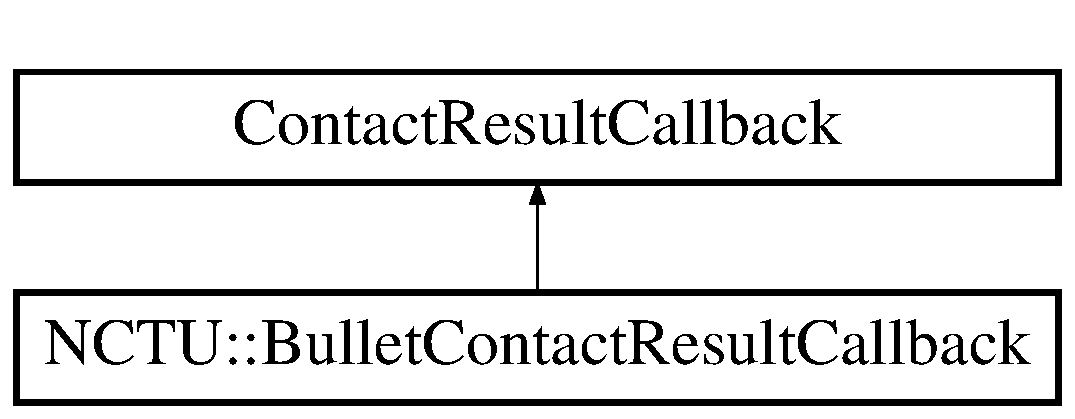
\includegraphics[height=2.000000cm]{struct_n_c_t_u_1_1_bullet_contact_result_callback}
\end{center}
\end{figure}
\subsection*{Public Member Functions}
\begin{DoxyCompactItemize}
\item 
\hyperlink{struct_n_c_t_u_1_1_bullet_contact_result_callback_a97ca928726763f91f76e675fd4df48d3}{Bullet\+Contact\+Result\+Callback} (\hyperlink{class_n_c_t_u_1_1_bullet_obstacle}{Bullet\+Obstacle} $\ast$me, \hyperlink{class_n_c_t_u_1_1_obstacle}{Obstacle} $\ast$tgr)\hypertarget{struct_n_c_t_u_1_1_bullet_contact_result_callback_a97ca928726763f91f76e675fd4df48d3}{}\label{struct_n_c_t_u_1_1_bullet_contact_result_callback_a97ca928726763f91f76e675fd4df48d3}

\begin{DoxyCompactList}\small\item\em handle contact result \end{DoxyCompactList}\item 
bt\+Scalar {\bfseries add\+Single\+Result} (bt\+Manifold\+Point \&cp, const bt\+Collision\+Object\+Wrapper $\ast$col\+Obj0\+Wrap, int part\+Id0, int index0, const bt\+Collision\+Object\+Wrapper $\ast$col\+Obj1\+Wrap, int part\+Id1, int index1)\hypertarget{struct_n_c_t_u_1_1_bullet_contact_result_callback_a7d692fc1c76a971ae37b65d1d711f349}{}\label{struct_n_c_t_u_1_1_bullet_contact_result_callback_a7d692fc1c76a971ae37b65d1d711f349}

\end{DoxyCompactItemize}
\subsection*{Public Attributes}
\begin{DoxyCompactItemize}
\item 
\hyperlink{class_n_c_t_u_1_1_obstacle}{Obstacle} $\ast$ \hyperlink{struct_n_c_t_u_1_1_bullet_contact_result_callback_a4b87f68a3e61872f1cfeb8e8b45d7933}{m\+Object}\hypertarget{struct_n_c_t_u_1_1_bullet_contact_result_callback_a4b87f68a3e61872f1cfeb8e8b45d7933}{}\label{struct_n_c_t_u_1_1_bullet_contact_result_callback_a4b87f68a3e61872f1cfeb8e8b45d7933}

\begin{DoxyCompactList}\small\item\em pointer to the obstacle \end{DoxyCompactList}\item 
\hyperlink{class_n_c_t_u_1_1_bullet_obstacle}{Bullet\+Obstacle} $\ast$ \hyperlink{struct_n_c_t_u_1_1_bullet_contact_result_callback_a352bd10d219aeb087061f93d65bb3618}{m\+Subject}\hypertarget{struct_n_c_t_u_1_1_bullet_contact_result_callback_a352bd10d219aeb087061f93d65bb3618}{}\label{struct_n_c_t_u_1_1_bullet_contact_result_callback_a352bd10d219aeb087061f93d65bb3618}

\begin{DoxyCompactList}\small\item\em pointer to the bullet \end{DoxyCompactList}\end{DoxyCompactItemize}


\subsection{Detailed Description}
callback for bullet-\/obstacle contact 

The documentation for this struct was generated from the following files\+:\begin{DoxyCompactItemize}
\item 
N\+C\+T\+U\+Obstacle/include/N\+C\+T\+U\+Obstacle\+Callback.\+h\item 
N\+C\+T\+U\+Obstacle/src/N\+C\+T\+U\+Obstacle\+Callback.\+cpp\end{DoxyCompactItemize}

\hypertarget{class_n_c_t_u_1_1_bullet_obstacle}{}\section{N\+C\+TU\+:\+:Bullet\+Obstacle Class Reference}
\label{class_n_c_t_u_1_1_bullet_obstacle}\index{N\+C\+T\+U\+::\+Bullet\+Obstacle@{N\+C\+T\+U\+::\+Bullet\+Obstacle}}


bullet obstacle  




{\ttfamily \#include $<$N\+C\+T\+U\+Bullet\+Obstacle.\+h$>$}

Inheritance diagram for N\+C\+TU\+:\+:Bullet\+Obstacle\+:\begin{figure}[H]
\begin{center}
\leavevmode
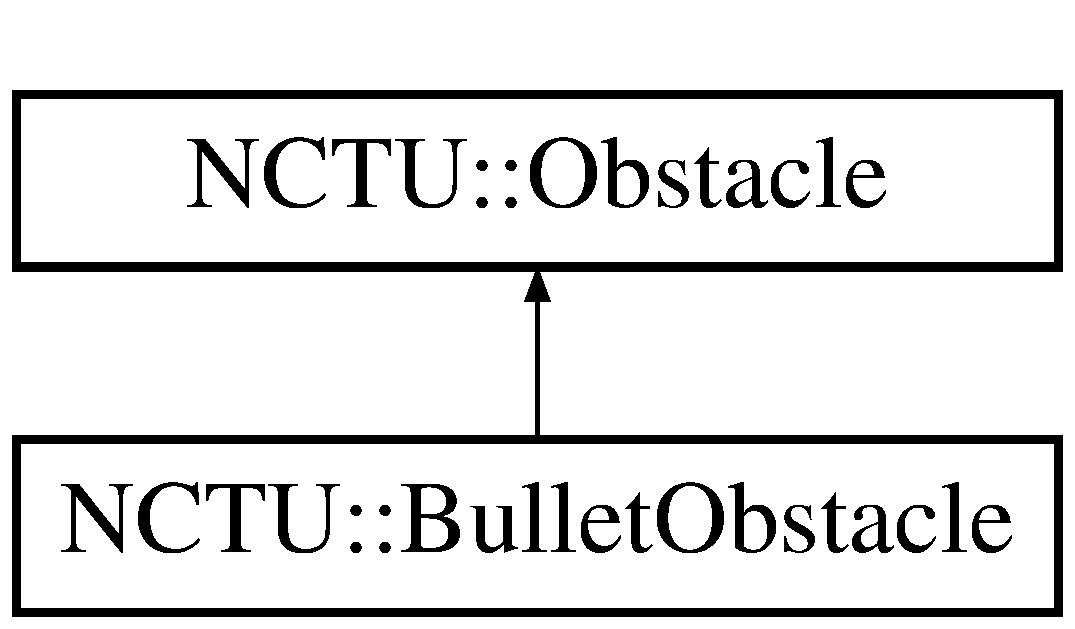
\includegraphics[height=2.000000cm]{class_n_c_t_u_1_1_bullet_obstacle}
\end{center}
\end{figure}
\subsection*{Public Member Functions}
\begin{DoxyCompactItemize}
\item 
\hyperlink{class_n_c_t_u_1_1_bullet_obstacle_a8ceaf3442116803582d703e6326b610a}{Bullet\+Obstacle} (\hyperlink{class_n_c_t_u_1_1_obstacle_manager}{Obstacle\+Manager} $\ast$mgmt, Ogre\+::\+Real restitution, Ogre\+::\+Real friction, Ogre\+::\+Real mass, I\+N\+D\+E\+X\+\_\+\+T\+Y\+PE index, Hp\+Type bullet\+Type, const Ogre\+::\+Vector3 \&position, Ogre\+::\+Real radius, const Ogre\+::\+Quaternion \&orientation)
\begin{DoxyCompactList}\small\item\em constructor \end{DoxyCompactList}\item 
virtual void \hyperlink{class_n_c_t_u_1_1_bullet_obstacle_a0e7b291970133412b00a30e8c5f65a19}{set\+Scale} (const Ogre\+::\+Vector3 \&)\hypertarget{class_n_c_t_u_1_1_bullet_obstacle_a0e7b291970133412b00a30e8c5f65a19}{}\label{class_n_c_t_u_1_1_bullet_obstacle_a0e7b291970133412b00a30e8c5f65a19}

\begin{DoxyCompactList}\small\item\em set obstacle scale \end{DoxyCompactList}\item 
virtual void \hyperlink{class_n_c_t_u_1_1_bullet_obstacle_a51c61e74c5e7b6918ea98343109cee50}{set\+Bullet\+Iterator} (std\+::list$<$ \hyperlink{class_n_c_t_u_1_1_bullet_obstacle}{Bullet\+Obstacle} $\ast$ $>$\+::iterator it)\hypertarget{class_n_c_t_u_1_1_bullet_obstacle_a51c61e74c5e7b6918ea98343109cee50}{}\label{class_n_c_t_u_1_1_bullet_obstacle_a51c61e74c5e7b6918ea98343109cee50}

\begin{DoxyCompactList}\small\item\em set bullet interator for manager \end{DoxyCompactList}\item 
virtual void \hyperlink{class_n_c_t_u_1_1_bullet_obstacle_afb9241ee7ed793b39cb8f60b5f1132ac}{on\+Bullet\+Hit} (\hyperlink{class_n_c_t_u_1_1_bullet_obstacle}{Bullet\+Obstacle} $\ast$, \hyperlink{class_n_c_t_u_1_1_obstacle}{Obstacle} $\ast$)\hypertarget{class_n_c_t_u_1_1_bullet_obstacle_afb9241ee7ed793b39cb8f60b5f1132ac}{}\label{class_n_c_t_u_1_1_bullet_obstacle_afb9241ee7ed793b39cb8f60b5f1132ac}

\begin{DoxyCompactList}\small\item\em process when bullet hit \end{DoxyCompactList}\item 
virtual bool \hyperlink{class_n_c_t_u_1_1_bullet_obstacle_a40e7d8af32475bc9520ead568771f64c}{is\+Alive} () const \hypertarget{class_n_c_t_u_1_1_bullet_obstacle_a40e7d8af32475bc9520ead568771f64c}{}\label{class_n_c_t_u_1_1_bullet_obstacle_a40e7d8af32475bc9520ead568771f64c}

\begin{DoxyCompactList}\small\item\em is bullet alive? \end{DoxyCompactList}\item 
virtual void \hyperlink{class_n_c_t_u_1_1_bullet_obstacle_a149609db8052addfcfebe2e24858fe20}{clean\+Up} ()\hypertarget{class_n_c_t_u_1_1_bullet_obstacle_a149609db8052addfcfebe2e24858fe20}{}\label{class_n_c_t_u_1_1_bullet_obstacle_a149609db8052addfcfebe2e24858fe20}

\begin{DoxyCompactList}\small\item\em clean up routine \end{DoxyCompactList}\item 
virtual Hp\+Type \hyperlink{class_n_c_t_u_1_1_bullet_obstacle_ad39ecce6671c5d1ea03ff5d017a7f475}{get\+Bullet\+Type} () const \hypertarget{class_n_c_t_u_1_1_bullet_obstacle_ad39ecce6671c5d1ea03ff5d017a7f475}{}\label{class_n_c_t_u_1_1_bullet_obstacle_ad39ecce6671c5d1ea03ff5d017a7f475}

\begin{DoxyCompactList}\small\item\em get the bullet hp type \end{DoxyCompactList}\item 
virtual void \hyperlink{class_n_c_t_u_1_1_bullet_obstacle_a749649fe487147408344fb4dfe3021cf}{update\+Life\+Time} (const Ogre\+::\+Frame\+Event \&evt)\hypertarget{class_n_c_t_u_1_1_bullet_obstacle_a749649fe487147408344fb4dfe3021cf}{}\label{class_n_c_t_u_1_1_bullet_obstacle_a749649fe487147408344fb4dfe3021cf}

\begin{DoxyCompactList}\small\item\em update life time \end{DoxyCompactList}\item 
virtual bool \hyperlink{class_n_c_t_u_1_1_bullet_obstacle_abf28165332c4599dad8a3b92cfb8fac8}{can\+Be\+Shoot} () const \hypertarget{class_n_c_t_u_1_1_bullet_obstacle_abf28165332c4599dad8a3b92cfb8fac8}{}\label{class_n_c_t_u_1_1_bullet_obstacle_abf28165332c4599dad8a3b92cfb8fac8}

\begin{DoxyCompactList}\small\item\em is this object can be shoot? \end{DoxyCompactList}\item 
virtual bool \hyperlink{class_n_c_t_u_1_1_bullet_obstacle_ac6d90f267ebd087d5322977344e69e59}{can\+Stand\+On} () const \hypertarget{class_n_c_t_u_1_1_bullet_obstacle_ac6d90f267ebd087d5322977344e69e59}{}\label{class_n_c_t_u_1_1_bullet_obstacle_ac6d90f267ebd087d5322977344e69e59}

\begin{DoxyCompactList}\small\item\em is this object can be standed on? \end{DoxyCompactList}\item 
virtual bool \hyperlink{class_n_c_t_u_1_1_bullet_obstacle_ae9fbd7f7ad7d5e58df1c5b28eaaf4bd5}{can\+Cause\+Dead} () const \hypertarget{class_n_c_t_u_1_1_bullet_obstacle_ae9fbd7f7ad7d5e58df1c5b28eaaf4bd5}{}\label{class_n_c_t_u_1_1_bullet_obstacle_ae9fbd7f7ad7d5e58df1c5b28eaaf4bd5}

\begin{DoxyCompactList}\small\item\em is this object can cause dead? \end{DoxyCompactList}\end{DoxyCompactItemize}
\subsection*{Static Public Member Functions}
\begin{DoxyCompactItemize}
\item 
static void \hyperlink{class_n_c_t_u_1_1_bullet_obstacle_a1b60b1c4c71033108c7f63e7722243bb}{set\+Handler\+Bullet\+Hit} (Bullet\+Hit\+Handler handler)\hypertarget{class_n_c_t_u_1_1_bullet_obstacle_a1b60b1c4c71033108c7f63e7722243bb}{}\label{class_n_c_t_u_1_1_bullet_obstacle_a1b60b1c4c71033108c7f63e7722243bb}

\begin{DoxyCompactList}\small\item\em set handler when bullet hit \end{DoxyCompactList}\end{DoxyCompactItemize}
\subsection*{Protected Member Functions}
\begin{DoxyCompactItemize}
\item 
virtual void \hyperlink{class_n_c_t_u_1_1_bullet_obstacle_a5b600a79973854cdc0dad76cbe8d77a6}{on\+Life\+End} ()\hypertarget{class_n_c_t_u_1_1_bullet_obstacle_a5b600a79973854cdc0dad76cbe8d77a6}{}\label{class_n_c_t_u_1_1_bullet_obstacle_a5b600a79973854cdc0dad76cbe8d77a6}

\begin{DoxyCompactList}\small\item\em process when life ended \end{DoxyCompactList}\end{DoxyCompactItemize}
\subsection*{Protected Attributes}
\begin{DoxyCompactItemize}
\item 
int \hyperlink{class_n_c_t_u_1_1_bullet_obstacle_a25cd3e3ee7a77a4bd51b652201d92dd5}{m\+Index}\hypertarget{class_n_c_t_u_1_1_bullet_obstacle_a25cd3e3ee7a77a4bd51b652201d92dd5}{}\label{class_n_c_t_u_1_1_bullet_obstacle_a25cd3e3ee7a77a4bd51b652201d92dd5}

\begin{DoxyCompactList}\small\item\em object index \end{DoxyCompactList}\item 
Ogre\+::\+Real \hyperlink{class_n_c_t_u_1_1_bullet_obstacle_a2ec54f863d2d04d11c4f1bf0771d36f7}{m\+Radius}\hypertarget{class_n_c_t_u_1_1_bullet_obstacle_a2ec54f863d2d04d11c4f1bf0771d36f7}{}\label{class_n_c_t_u_1_1_bullet_obstacle_a2ec54f863d2d04d11c4f1bf0771d36f7}

\begin{DoxyCompactList}\small\item\em bullet radius \end{DoxyCompactList}\item 
std\+::list$<$ \hyperlink{class_n_c_t_u_1_1_bullet_obstacle}{Bullet\+Obstacle} $\ast$ $>$\+::iterator \hyperlink{class_n_c_t_u_1_1_bullet_obstacle_ac56f8d89eea0be19564990b1a5459916}{m\+Bullet\+Iterator}\hypertarget{class_n_c_t_u_1_1_bullet_obstacle_ac56f8d89eea0be19564990b1a5459916}{}\label{class_n_c_t_u_1_1_bullet_obstacle_ac56f8d89eea0be19564990b1a5459916}

\begin{DoxyCompactList}\small\item\em iterator for manager \end{DoxyCompactList}\item 
bool \hyperlink{class_n_c_t_u_1_1_bullet_obstacle_aba277c2a430e552a2bbcd4ac0d800d0c}{m\+Hit}\hypertarget{class_n_c_t_u_1_1_bullet_obstacle_aba277c2a430e552a2bbcd4ac0d800d0c}{}\label{class_n_c_t_u_1_1_bullet_obstacle_aba277c2a430e552a2bbcd4ac0d800d0c}

\begin{DoxyCompactList}\small\item\em is bullet hit something? \end{DoxyCompactList}\item 
Hp\+Type \hyperlink{class_n_c_t_u_1_1_bullet_obstacle_a8b634c38b5e2172f220709afd534f2c6}{m\+Bullet\+Type}\hypertarget{class_n_c_t_u_1_1_bullet_obstacle_a8b634c38b5e2172f220709afd534f2c6}{}\label{class_n_c_t_u_1_1_bullet_obstacle_a8b634c38b5e2172f220709afd534f2c6}

\begin{DoxyCompactList}\small\item\em the hp type for bullet \end{DoxyCompactList}\item 
Ogre\+::\+Real \hyperlink{class_n_c_t_u_1_1_bullet_obstacle_a95dac20c5d14bb5db86aa18835d78004}{m\+Particle\+Life\+Time}\hypertarget{class_n_c_t_u_1_1_bullet_obstacle_a95dac20c5d14bb5db86aa18835d78004}{}\label{class_n_c_t_u_1_1_bullet_obstacle_a95dac20c5d14bb5db86aa18835d78004}

\begin{DoxyCompactList}\small\item\em life time for particle system \end{DoxyCompactList}\end{DoxyCompactItemize}
\subsection*{Static Protected Attributes}
\begin{DoxyCompactItemize}
\item 
static Bullet\+Hit\+Handler \hyperlink{class_n_c_t_u_1_1_bullet_obstacle_a1756674a45f79c57e9815756fecc55f4}{m\+Bullet\+Hit\+Handler} = nullptr\hypertarget{class_n_c_t_u_1_1_bullet_obstacle_a1756674a45f79c57e9815756fecc55f4}{}\label{class_n_c_t_u_1_1_bullet_obstacle_a1756674a45f79c57e9815756fecc55f4}

\begin{DoxyCompactList}\small\item\em the bullet-\/hit handler \end{DoxyCompactList}\end{DoxyCompactItemize}
\subsection*{Additional Inherited Members}


\subsection{Detailed Description}
bullet obstacle 

\subsection{Constructor \& Destructor Documentation}
\index{N\+C\+T\+U\+::\+Bullet\+Obstacle@{N\+C\+T\+U\+::\+Bullet\+Obstacle}!Bullet\+Obstacle@{Bullet\+Obstacle}}
\index{Bullet\+Obstacle@{Bullet\+Obstacle}!N\+C\+T\+U\+::\+Bullet\+Obstacle@{N\+C\+T\+U\+::\+Bullet\+Obstacle}}
\subsubsection[{\texorpdfstring{Bullet\+Obstacle(\+Obstacle\+Manager $\ast$mgmt, Ogre\+::\+Real restitution, Ogre\+::\+Real friction, Ogre\+::\+Real mass, I\+N\+D\+E\+X\+\_\+\+T\+Y\+P\+E index, Hp\+Type bullet\+Type, const Ogre\+::\+Vector3 \&position, Ogre\+::\+Real radius, const Ogre\+::\+Quaternion \&orientation)}{BulletObstacle(ObstacleManager *mgmt, Ogre::Real restitution, Ogre::Real friction, Ogre::Real mass, INDEX_TYPE index, HpType bulletType, const Ogre::Vector3 &position, Ogre::Real radius, const Ogre::Quaternion &orientation)}}]{\setlength{\rightskip}{0pt plus 5cm}Bullet\+Obstacle\+::\+Bullet\+Obstacle (
\begin{DoxyParamCaption}
\item[{{\bf Obstacle\+Manager} $\ast$}]{mgmt, }
\item[{Ogre\+::\+Real}]{restitution, }
\item[{Ogre\+::\+Real}]{friction, }
\item[{Ogre\+::\+Real}]{mass, }
\item[{I\+N\+D\+E\+X\+\_\+\+T\+Y\+PE}]{index, }
\item[{Hp\+Type}]{bullet\+Type, }
\item[{const Ogre\+::\+Vector3 \&}]{position, }
\item[{Ogre\+::\+Real}]{radius, }
\item[{const Ogre\+::\+Quaternion \&}]{orientation}
\end{DoxyParamCaption}
)}\hypertarget{class_n_c_t_u_1_1_bullet_obstacle_a8ceaf3442116803582d703e6326b610a}{}\label{class_n_c_t_u_1_1_bullet_obstacle_a8ceaf3442116803582d703e6326b610a}


constructor 

Create a bullet obstacle (full) 

The documentation for this class was generated from the following files\+:\begin{DoxyCompactItemize}
\item 
N\+C\+T\+U\+Obstacle/include/N\+C\+T\+U\+Bullet\+Obstacle.\+h\item 
N\+C\+T\+U\+Obstacle/src/N\+C\+T\+U\+Bullet\+Obstacle.\+cpp\end{DoxyCompactItemize}

\hypertarget{class_camera_motion}{}\section{Camera\+Motion Class Reference}
\label{class_camera_motion}\index{Camera\+Motion@{Camera\+Motion}}


A class that stores and indicates that the player motion.  




{\ttfamily \#include $<$Camera\+Motion.\+h$>$}

\subsection*{Public Member Functions}
\begin{DoxyCompactItemize}
\item 
void \hyperlink{class_camera_motion_a2a388dd7c3bc04330a6b421d198d0548}{record} (const Ogre\+::\+Vector3 \&v)\hypertarget{class_camera_motion_a2a388dd7c3bc04330a6b421d198d0548}{}\label{class_camera_motion_a2a388dd7c3bc04330a6b421d198d0548}

\begin{DoxyCompactList}\small\item\em record the motion information from Vector3 \end{DoxyCompactList}\item 
bool \hyperlink{class_camera_motion_a66657c2fe27ad0aeb400dacf59cd5184}{is\+Down} () const \hypertarget{class_camera_motion_a66657c2fe27ad0aeb400dacf59cd5184}{}\label{class_camera_motion_a66657c2fe27ad0aeb400dacf59cd5184}

\begin{DoxyCompactList}\small\item\em return whether the motion is down or not \end{DoxyCompactList}\end{DoxyCompactItemize}
\subsection*{Static Public Attributes}
\begin{DoxyCompactItemize}
\item 
static const int \hyperlink{class_camera_motion_a03765a27a1c9820d9c52883a5b671331}{M\+A\+X\+\_\+\+R\+E\+C\+O\+RD} = 10\hypertarget{class_camera_motion_a03765a27a1c9820d9c52883a5b671331}{}\label{class_camera_motion_a03765a27a1c9820d9c52883a5b671331}

\begin{DoxyCompactList}\small\item\em how many motion record stored interally \end{DoxyCompactList}\item 
static const int \hyperlink{class_camera_motion_a4dbc2da5975bdd4e5dea9f2d5d3f8d78}{R\+E\+Q\+\_\+\+C\+O\+U\+NT} = 8\hypertarget{class_camera_motion_a4dbc2da5975bdd4e5dea9f2d5d3f8d78}{}\label{class_camera_motion_a4dbc2da5975bdd4e5dea9f2d5d3f8d78}

\begin{DoxyCompactList}\small\item\em threshold for motion jugdement \end{DoxyCompactList}\end{DoxyCompactItemize}


\subsection{Detailed Description}
A class that stores and indicates that the player motion. 

The documentation for this class was generated from the following files\+:\begin{DoxyCompactItemize}
\item 
programs/\+Obstacle/include/Camera\+Motion.\+h\item 
programs/\+Obstacle/source/Camera\+Motion.\+cpp\end{DoxyCompactItemize}

\hypertarget{class_n_c_t_u_1_1_cube_obstacle}{}\section{N\+C\+TU\+:\+:Cube\+Obstacle Class Reference}
\label{class_n_c_t_u_1_1_cube_obstacle}\index{N\+C\+T\+U\+::\+Cube\+Obstacle@{N\+C\+T\+U\+::\+Cube\+Obstacle}}


cube obstacle for testing  




{\ttfamily \#include $<$N\+C\+T\+U\+Cube\+Obstacle.\+h$>$}

Inheritance diagram for N\+C\+TU\+:\+:Cube\+Obstacle\+:\begin{figure}[H]
\begin{center}
\leavevmode
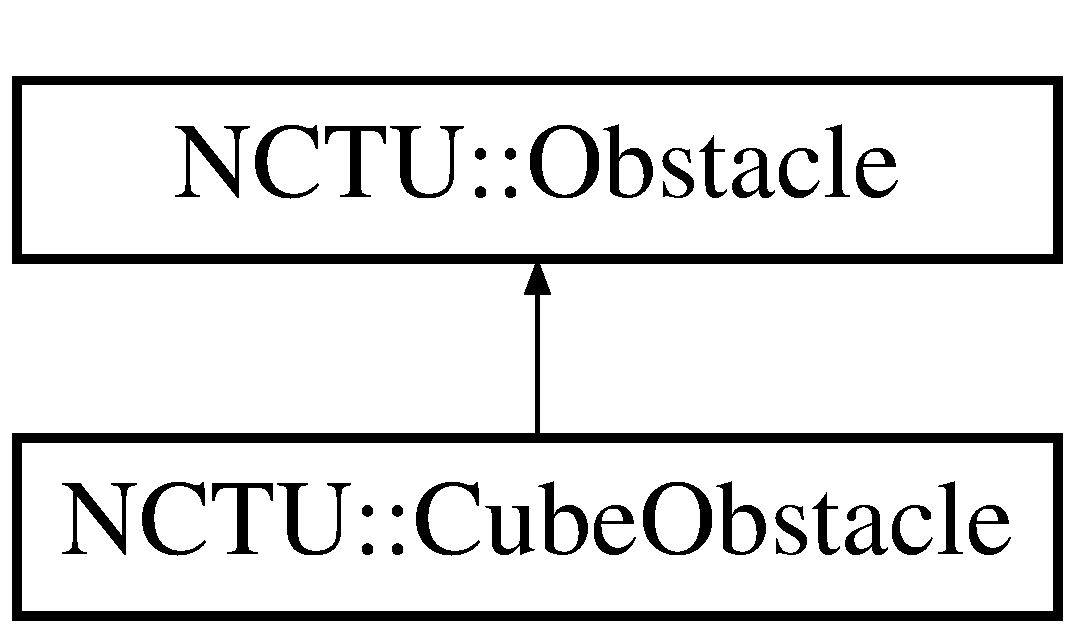
\includegraphics[height=2.000000cm]{class_n_c_t_u_1_1_cube_obstacle}
\end{center}
\end{figure}
\subsection*{Public Member Functions}
\begin{DoxyCompactItemize}
\item 
\hyperlink{class_n_c_t_u_1_1_cube_obstacle_ac6d8fba5dc23abaebe8c07bc3175c75a}{Cube\+Obstacle} (\hyperlink{class_n_c_t_u_1_1_obstacle_manager}{Obstacle\+Manager} $\ast$mgmt, Ogre\+::\+Real restitution, Ogre\+::\+Real friction, Ogre\+::\+Real mass, I\+N\+D\+E\+X\+\_\+\+T\+Y\+PE index, const Ogre\+::\+Vector3 \&position, const Ogre\+::\+Vector3 \&size, const Ogre\+::\+Quaternion \&orientation)
\begin{DoxyCompactList}\small\item\em constructor \end{DoxyCompactList}\item 
virtual void \hyperlink{class_n_c_t_u_1_1_cube_obstacle_a739b5db3f9338a13ddd40471f3e0d3b0}{set\+Scale} (const Ogre\+::\+Vector3 \&)\hypertarget{class_n_c_t_u_1_1_cube_obstacle_a739b5db3f9338a13ddd40471f3e0d3b0}{}\label{class_n_c_t_u_1_1_cube_obstacle_a739b5db3f9338a13ddd40471f3e0d3b0}

\begin{DoxyCompactList}\small\item\em set scale for this object \end{DoxyCompactList}\end{DoxyCompactItemize}
\subsection*{Protected Attributes}
\begin{DoxyCompactItemize}
\item 
I\+N\+D\+E\+X\+\_\+\+T\+Y\+PE \hyperlink{class_n_c_t_u_1_1_cube_obstacle_a0aa0b74760857bd929749844278f6cfc}{m\+Index}\hypertarget{class_n_c_t_u_1_1_cube_obstacle_a0aa0b74760857bd929749844278f6cfc}{}\label{class_n_c_t_u_1_1_cube_obstacle_a0aa0b74760857bd929749844278f6cfc}

\begin{DoxyCompactList}\small\item\em object index \end{DoxyCompactList}\item 
Ogre\+::\+Vector3 \hyperlink{class_n_c_t_u_1_1_cube_obstacle_a372291c45b79d711ab9c45214cd013b8}{m\+Init\+Scale}\hypertarget{class_n_c_t_u_1_1_cube_obstacle_a372291c45b79d711ab9c45214cd013b8}{}\label{class_n_c_t_u_1_1_cube_obstacle_a372291c45b79d711ab9c45214cd013b8}

\begin{DoxyCompactList}\small\item\em initial scale for this object \end{DoxyCompactList}\end{DoxyCompactItemize}
\subsection*{Additional Inherited Members}


\subsection{Detailed Description}
cube obstacle for testing 

\subsection{Constructor \& Destructor Documentation}
\index{N\+C\+T\+U\+::\+Cube\+Obstacle@{N\+C\+T\+U\+::\+Cube\+Obstacle}!Cube\+Obstacle@{Cube\+Obstacle}}
\index{Cube\+Obstacle@{Cube\+Obstacle}!N\+C\+T\+U\+::\+Cube\+Obstacle@{N\+C\+T\+U\+::\+Cube\+Obstacle}}
\subsubsection[{\texorpdfstring{Cube\+Obstacle(\+Obstacle\+Manager $\ast$mgmt, Ogre\+::\+Real restitution, Ogre\+::\+Real friction, Ogre\+::\+Real mass, I\+N\+D\+E\+X\+\_\+\+T\+Y\+P\+E index, const Ogre\+::\+Vector3 \&position, const Ogre\+::\+Vector3 \&size, const Ogre\+::\+Quaternion \&orientation)}{CubeObstacle(ObstacleManager *mgmt, Ogre::Real restitution, Ogre::Real friction, Ogre::Real mass, INDEX_TYPE index, const Ogre::Vector3 &position, const Ogre::Vector3 &size, const Ogre::Quaternion &orientation)}}]{\setlength{\rightskip}{0pt plus 5cm}Cube\+Obstacle\+::\+Cube\+Obstacle (
\begin{DoxyParamCaption}
\item[{{\bf Obstacle\+Manager} $\ast$}]{mgmt, }
\item[{Ogre\+::\+Real}]{restitution, }
\item[{Ogre\+::\+Real}]{friction, }
\item[{Ogre\+::\+Real}]{mass, }
\item[{I\+N\+D\+E\+X\+\_\+\+T\+Y\+PE}]{index, }
\item[{const Ogre\+::\+Vector3 \&}]{position, }
\item[{const Ogre\+::\+Vector3 \&}]{size, }
\item[{const Ogre\+::\+Quaternion \&}]{orientation}
\end{DoxyParamCaption}
)}\hypertarget{class_n_c_t_u_1_1_cube_obstacle_ac6d8fba5dc23abaebe8c07bc3175c75a}{}\label{class_n_c_t_u_1_1_cube_obstacle_ac6d8fba5dc23abaebe8c07bc3175c75a}


constructor 

Create a cube obstacle (full) 

The documentation for this class was generated from the following files\+:\begin{DoxyCompactItemize}
\item 
N\+C\+T\+U\+Obstacle/include/N\+C\+T\+U\+Cube\+Obstacle.\+h\item 
N\+C\+T\+U\+Obstacle/src/N\+C\+T\+U\+Cube\+Obstacle.\+cpp\end{DoxyCompactItemize}

\hypertarget{class_ogre_1_1_dot_scene_loader}{}\section{Ogre\+:\+:Dot\+Scene\+Loader Class Reference}
\label{class_ogre_1_1_dot_scene_loader}\index{Ogre\+::\+Dot\+Scene\+Loader@{Ogre\+::\+Dot\+Scene\+Loader}}


main class for Dot\+Scene reading  




{\ttfamily \#include $<$Dot\+Scene\+Loader.\+h$>$}

\subsection*{Public Member Functions}
\begin{DoxyCompactItemize}
\item 
\hyperlink{class_ogre_1_1_dot_scene_loader_a4d3297139bca45e1130443d79b7b2e70}{Dot\+Scene\+Loader} ()\hypertarget{class_ogre_1_1_dot_scene_loader_a4d3297139bca45e1130443d79b7b2e70}{}\label{class_ogre_1_1_dot_scene_loader_a4d3297139bca45e1130443d79b7b2e70}

\begin{DoxyCompactList}\small\item\em contructor \end{DoxyCompactList}\item 
virtual \hyperlink{class_ogre_1_1_dot_scene_loader_a6a2e576a1adac9e7dd9c59548c02df47}{$\sim$\+Dot\+Scene\+Loader} ()\hypertarget{class_ogre_1_1_dot_scene_loader_a6a2e576a1adac9e7dd9c59548c02df47}{}\label{class_ogre_1_1_dot_scene_loader_a6a2e576a1adac9e7dd9c59548c02df47}

\begin{DoxyCompactList}\small\item\em destructor \end{DoxyCompactList}\item 
void \hyperlink{class_ogre_1_1_dot_scene_loader_a980e8d431568586740534e0c2fd596b1}{parse\+Dot\+Scene} (const String \&Scene\+Name, const String \&group\+Name, Scene\+Manager $\ast$your\+Scene\+Mgr, \hyperlink{class_n_c_t_u_1_1_obstacle_manager}{N\+C\+T\+U\+::\+Obstacle\+Manager} $\ast$obstacle\+Mgr, Scene\+Node $\ast$p\+Attach\+Node=N\+U\+LL, const String \&s\+Prepend\+Node=\char`\"{}\char`\"{})\hypertarget{class_ogre_1_1_dot_scene_loader_a980e8d431568586740534e0c2fd596b1}{}\label{class_ogre_1_1_dot_scene_loader_a980e8d431568586740534e0c2fd596b1}

\begin{DoxyCompactList}\small\item\em parse the given Dot\+Scene file \end{DoxyCompactList}\item 
String \hyperlink{class_ogre_1_1_dot_scene_loader_ac4d94f0ab478ee808f63e5cf43755cf9}{get\+Property} (const String \&nd\+Nm, const String \&prop)\hypertarget{class_ogre_1_1_dot_scene_loader_ac4d94f0ab478ee808f63e5cf43755cf9}{}\label{class_ogre_1_1_dot_scene_loader_ac4d94f0ab478ee808f63e5cf43755cf9}

\begin{DoxyCompactList}\small\item\em get property of a node \end{DoxyCompactList}\item 
void \hyperlink{class_ogre_1_1_dot_scene_loader_a4e6b3ce29f7cf2a24717290f89c3b834}{destroy\+Dedicated\+Scene\+Nodes} ()\hypertarget{class_ogre_1_1_dot_scene_loader_a4e6b3ce29f7cf2a24717290f89c3b834}{}\label{class_ogre_1_1_dot_scene_loader_a4e6b3ce29f7cf2a24717290f89c3b834}

\begin{DoxyCompactList}\small\item\em destory the scene nodes without physics objects \end{DoxyCompactList}\item 
void \hyperlink{class_ogre_1_1_dot_scene_loader_a52b96034fb06a7e5a93cd22592c16908}{load\+Dummy\+Scene} ()\hypertarget{class_ogre_1_1_dot_scene_loader_a52b96034fb06a7e5a93cd22592c16908}{}\label{class_ogre_1_1_dot_scene_loader_a52b96034fb06a7e5a93cd22592c16908}

\begin{DoxyCompactList}\small\item\em load a dummy scene with player only \end{DoxyCompactList}\end{DoxyCompactItemize}
\subsection*{Public Attributes}
\begin{DoxyCompactItemize}
\item 
std\+::vector$<$ \hyperlink{class_ogre_1_1node_property}{node\+Property} $>$ \hyperlink{class_ogre_1_1_dot_scene_loader_a8aef910eb41e3aa2685d24b60aad4363}{node\+Properties}\hypertarget{class_ogre_1_1_dot_scene_loader_a8aef910eb41e3aa2685d24b60aad4363}{}\label{class_ogre_1_1_dot_scene_loader_a8aef910eb41e3aa2685d24b60aad4363}

\begin{DoxyCompactList}\small\item\em array of node properties \end{DoxyCompactList}\item 
std\+::vector$<$ String $>$ \hyperlink{class_ogre_1_1_dot_scene_loader_a23a316c6eea305326b3be89113bde609}{static\+Objects}\hypertarget{class_ogre_1_1_dot_scene_loader_a23a316c6eea305326b3be89113bde609}{}\label{class_ogre_1_1_dot_scene_loader_a23a316c6eea305326b3be89113bde609}

\begin{DoxyCompactList}\small\item\em array of static objects \end{DoxyCompactList}\item 
std\+::vector$<$ String $>$ \hyperlink{class_ogre_1_1_dot_scene_loader_a95daf060322172a14ee6292e64e2c791}{dynamic\+Objects}\hypertarget{class_ogre_1_1_dot_scene_loader_a95daf060322172a14ee6292e64e2c791}{}\label{class_ogre_1_1_dot_scene_loader_a95daf060322172a14ee6292e64e2c791}

\begin{DoxyCompactList}\small\item\em array of dynamic objects \end{DoxyCompactList}\item 
\hyperlink{classprop_map}{prop\+Map}$<$ String, \hyperlink{class_ogre_1_1_general_property}{General\+Property} $>$ \hyperlink{class_ogre_1_1_dot_scene_loader_a98b2228adaa994df2d99979afc5e7eb1}{m\+General\+Props}\hypertarget{class_ogre_1_1_dot_scene_loader_a98b2228adaa994df2d99979afc5e7eb1}{}\label{class_ogre_1_1_dot_scene_loader_a98b2228adaa994df2d99979afc5e7eb1}

\begin{DoxyCompactList}\small\item\em general properties \end{DoxyCompactList}\end{DoxyCompactItemize}
\subsection*{Protected Member Functions}
\begin{DoxyCompactItemize}
\item 
void \hyperlink{class_ogre_1_1_dot_scene_loader_a05a2ebb03c3be72af3ee072fc7211d06}{process\+Scene} (Ti\+Xml\+Element $\ast$X\+M\+L\+Root)\hypertarget{class_ogre_1_1_dot_scene_loader_a05a2ebb03c3be72af3ee072fc7211d06}{}\label{class_ogre_1_1_dot_scene_loader_a05a2ebb03c3be72af3ee072fc7211d06}

\begin{DoxyCompactList}\small\item\em process a scene section \end{DoxyCompactList}\item 
void \hyperlink{class_ogre_1_1_dot_scene_loader_acdcc1c065c8733156bb97c17c07f6dec}{process\+Nodes} (Ti\+Xml\+Element $\ast$X\+M\+L\+Node)\hypertarget{class_ogre_1_1_dot_scene_loader_acdcc1c065c8733156bb97c17c07f6dec}{}\label{class_ogre_1_1_dot_scene_loader_acdcc1c065c8733156bb97c17c07f6dec}

\begin{DoxyCompactList}\small\item\em process a nodes section \end{DoxyCompactList}\item 
void \hyperlink{class_ogre_1_1_dot_scene_loader_a1627804a409b0dccd5598323f3d85359}{process\+Externals} (Ti\+Xml\+Element $\ast$X\+M\+L\+Node)
\begin{DoxyCompactList}\small\item\em process a externals section \end{DoxyCompactList}\item 
void \hyperlink{class_ogre_1_1_dot_scene_loader_a6c541dcb42d29071b2556b85f8cd1a62}{process\+Environment} (Ti\+Xml\+Element $\ast$X\+M\+L\+Node)
\begin{DoxyCompactList}\small\item\em process a environment section \end{DoxyCompactList}\item 
void \hyperlink{class_ogre_1_1_dot_scene_loader_ad2f5858edce531f9a7be2e6ebdcebc5e}{process\+Terrain} (Ti\+Xml\+Element $\ast$X\+M\+L\+Node)
\begin{DoxyCompactList}\small\item\em process a terrian section \end{DoxyCompactList}\item 
void \hyperlink{class_ogre_1_1_dot_scene_loader_a24d6db1a195dea881b934753253e8e68}{process\+User\+Data\+Reference} (Ti\+Xml\+Element $\ast$X\+M\+L\+Node, Scene\+Node $\ast$p\+Parent=0)
\begin{DoxyCompactList}\small\item\em process user data reference \end{DoxyCompactList}\item 
void \hyperlink{class_ogre_1_1_dot_scene_loader_a4edd2c7fa8f951f7ecba5d6f8f841330}{process\+User\+Data\+Reference} (Ti\+Xml\+Element $\ast$X\+M\+L\+Node, Entity $\ast$p\+Entity)\hypertarget{class_ogre_1_1_dot_scene_loader_a4edd2c7fa8f951f7ecba5d6f8f841330}{}\label{class_ogre_1_1_dot_scene_loader_a4edd2c7fa8f951f7ecba5d6f8f841330}

\begin{DoxyCompactList}\small\item\em process user data reference \end{DoxyCompactList}\item 
void \hyperlink{class_ogre_1_1_dot_scene_loader_ad23d30b2c6ee9d24dabc89b28d9b61ed}{process\+Octree} (Ti\+Xml\+Element $\ast$X\+M\+L\+Node)
\begin{DoxyCompactList}\small\item\em process octree \end{DoxyCompactList}\item 
void \hyperlink{class_ogre_1_1_dot_scene_loader_a0861154e3d3cdfebdd886116a99d2ea9}{process\+Light} (Ti\+Xml\+Element $\ast$X\+M\+L\+Node, Scene\+Node $\ast$p\+Parent=0)\hypertarget{class_ogre_1_1_dot_scene_loader_a0861154e3d3cdfebdd886116a99d2ea9}{}\label{class_ogre_1_1_dot_scene_loader_a0861154e3d3cdfebdd886116a99d2ea9}

\begin{DoxyCompactList}\small\item\em process a light section \end{DoxyCompactList}\item 
void \hyperlink{class_ogre_1_1_dot_scene_loader_a92989e4631cd46d31337c006b46c1aea}{process\+Camera} (Ti\+Xml\+Element $\ast$X\+M\+L\+Node, Scene\+Node $\ast$p\+Parent=0)
\begin{DoxyCompactList}\small\item\em process a camera section \end{DoxyCompactList}\item 
void \hyperlink{class_ogre_1_1_dot_scene_loader_ae84828e86b8e34f1b43ff8e5fc006587}{process\+Node} (Ti\+Xml\+Element $\ast$X\+M\+L\+Node, Scene\+Node $\ast$p\+Parent=0)\hypertarget{class_ogre_1_1_dot_scene_loader_ae84828e86b8e34f1b43ff8e5fc006587}{}\label{class_ogre_1_1_dot_scene_loader_ae84828e86b8e34f1b43ff8e5fc006587}

\begin{DoxyCompactList}\small\item\em process a node section \end{DoxyCompactList}\item 
void \hyperlink{class_ogre_1_1_dot_scene_loader_a3f8227871f6a283222b1d0a88076d6d8}{process\+Look\+Target} (Ti\+Xml\+Element $\ast$X\+M\+L\+Node, Scene\+Node $\ast$p\+Parent)
\begin{DoxyCompactList}\small\item\em process look target \end{DoxyCompactList}\item 
void \hyperlink{class_ogre_1_1_dot_scene_loader_a8b9d37f443c59ea8409a7b2c954bc326}{process\+Track\+Target} (Ti\+Xml\+Element $\ast$X\+M\+L\+Node, Scene\+Node $\ast$p\+Parent)\hypertarget{class_ogre_1_1_dot_scene_loader_a8b9d37f443c59ea8409a7b2c954bc326}{}\label{class_ogre_1_1_dot_scene_loader_a8b9d37f443c59ea8409a7b2c954bc326}

\begin{DoxyCompactList}\small\item\em process track target \end{DoxyCompactList}\item 
Entity $\ast$ \hyperlink{class_ogre_1_1_dot_scene_loader_a5bda9ab5afc1f5e8ada8696739d7cf26}{process\+Entity} (Ti\+Xml\+Element $\ast$X\+M\+L\+Node, Scene\+Node $\ast$p\+Parent, const String \&name\+Prefix=\char`\"{}\char`\"{})\hypertarget{class_ogre_1_1_dot_scene_loader_a5bda9ab5afc1f5e8ada8696739d7cf26}{}\label{class_ogre_1_1_dot_scene_loader_a5bda9ab5afc1f5e8ada8696739d7cf26}

\begin{DoxyCompactList}\small\item\em process entity \end{DoxyCompactList}\item 
void \hyperlink{class_ogre_1_1_dot_scene_loader_a4aac1d9bbefcd0026a2f21005d587fe0}{process\+Particle\+System} (Ti\+Xml\+Element $\ast$X\+M\+L\+Node, Scene\+Node $\ast$p\+Parent)\hypertarget{class_ogre_1_1_dot_scene_loader_a4aac1d9bbefcd0026a2f21005d587fe0}{}\label{class_ogre_1_1_dot_scene_loader_a4aac1d9bbefcd0026a2f21005d587fe0}

\begin{DoxyCompactList}\small\item\em process particle system \end{DoxyCompactList}\item 
void \hyperlink{class_ogre_1_1_dot_scene_loader_a9b7c7ccd8f2724eb44dc9428ba6cb0d7}{process\+Billboard\+Set} (Ti\+Xml\+Element $\ast$X\+M\+L\+Node, Scene\+Node $\ast$p\+Parent)
\begin{DoxyCompactList}\small\item\em process billboard set \end{DoxyCompactList}\item 
void \hyperlink{class_ogre_1_1_dot_scene_loader_a8131406550814512ea64907b598b3f1c}{process\+Plane} (Ti\+Xml\+Element $\ast$X\+M\+L\+Node, Scene\+Node $\ast$p\+Parent)
\begin{DoxyCompactList}\small\item\em process plane \end{DoxyCompactList}\item 
void \hyperlink{class_ogre_1_1_dot_scene_loader_ac6f536ff0e073cf1d684027577561fb7}{process\+Fog} (Ti\+Xml\+Element $\ast$X\+M\+L\+Node)\hypertarget{class_ogre_1_1_dot_scene_loader_ac6f536ff0e073cf1d684027577561fb7}{}\label{class_ogre_1_1_dot_scene_loader_ac6f536ff0e073cf1d684027577561fb7}

\begin{DoxyCompactList}\small\item\em process fog \end{DoxyCompactList}\item 
void \hyperlink{class_ogre_1_1_dot_scene_loader_ab862c3347cbb0dfe2063afb2a382399f}{process\+Sky\+Box} (Ti\+Xml\+Element $\ast$X\+M\+L\+Node)\hypertarget{class_ogre_1_1_dot_scene_loader_ab862c3347cbb0dfe2063afb2a382399f}{}\label{class_ogre_1_1_dot_scene_loader_ab862c3347cbb0dfe2063afb2a382399f}

\begin{DoxyCompactList}\small\item\em process skybox \end{DoxyCompactList}\item 
void \hyperlink{class_ogre_1_1_dot_scene_loader_aa22fc5272abcfc46641659f0f830d150}{process\+Sky\+Dome} (Ti\+Xml\+Element $\ast$X\+M\+L\+Node)\hypertarget{class_ogre_1_1_dot_scene_loader_aa22fc5272abcfc46641659f0f830d150}{}\label{class_ogre_1_1_dot_scene_loader_aa22fc5272abcfc46641659f0f830d150}

\begin{DoxyCompactList}\small\item\em process sky dome \end{DoxyCompactList}\item 
void \hyperlink{class_ogre_1_1_dot_scene_loader_a3021c43d60580055e58cf14ded3bee23}{process\+Sky\+Plane} (Ti\+Xml\+Element $\ast$X\+M\+L\+Node)\hypertarget{class_ogre_1_1_dot_scene_loader_a3021c43d60580055e58cf14ded3bee23}{}\label{class_ogre_1_1_dot_scene_loader_a3021c43d60580055e58cf14ded3bee23}

\begin{DoxyCompactList}\small\item\em process sky plane \end{DoxyCompactList}\item 
void \hyperlink{class_ogre_1_1_dot_scene_loader_a0d8466f519cf49e4177369b542da50be}{process\+Clipping} (Ti\+Xml\+Element $\ast$X\+M\+L\+Node)
\begin{DoxyCompactList}\small\item\em process clipping \end{DoxyCompactList}\item 
void \hyperlink{class_ogre_1_1_dot_scene_loader_a5f7e231f59db99465f289f7f31f6cb83}{process\+Light\+Range} (Ti\+Xml\+Element $\ast$X\+M\+L\+Node, Light $\ast$p\+Light)\hypertarget{class_ogre_1_1_dot_scene_loader_a5f7e231f59db99465f289f7f31f6cb83}{}\label{class_ogre_1_1_dot_scene_loader_a5f7e231f59db99465f289f7f31f6cb83}

\begin{DoxyCompactList}\small\item\em process light range \end{DoxyCompactList}\item 
void \hyperlink{class_ogre_1_1_dot_scene_loader_af02d2e6e141232809a7c0d11461a6f88}{process\+Light\+Attenuation} (Ti\+Xml\+Element $\ast$X\+M\+L\+Node, Light $\ast$p\+Light)\hypertarget{class_ogre_1_1_dot_scene_loader_af02d2e6e141232809a7c0d11461a6f88}{}\label{class_ogre_1_1_dot_scene_loader_af02d2e6e141232809a7c0d11461a6f88}

\begin{DoxyCompactList}\small\item\em process light attenuation \end{DoxyCompactList}\item 
bool \hyperlink{class_ogre_1_1_dot_scene_loader_a31771f6a68683919b853c29a2acb8689}{process\+Obstacle\+Property} (Ti\+Xml\+Element $\ast$X\+M\+L\+Node, const String \&name, Scene\+Node $\ast$node, Entity $\ast$ent)\hypertarget{class_ogre_1_1_dot_scene_loader_a31771f6a68683919b853c29a2acb8689}{}\label{class_ogre_1_1_dot_scene_loader_a31771f6a68683919b853c29a2acb8689}

\begin{DoxyCompactList}\small\item\em process obstacle property \end{DoxyCompactList}\item 
void \hyperlink{class_ogre_1_1_dot_scene_loader_aa8c6a5f51bebc6b703cfbdfaaa6277c7}{process\+Obstacle\+Extra\+Field} (Ti\+Xml\+Element $\ast$X\+M\+L\+Node, \hyperlink{class_ogre_1_1_obstacle_property}{Obstacle\+Property} \&prop, bool save\+As\+General=false)\hypertarget{class_ogre_1_1_dot_scene_loader_aa8c6a5f51bebc6b703cfbdfaaa6277c7}{}\label{class_ogre_1_1_dot_scene_loader_aa8c6a5f51bebc6b703cfbdfaaa6277c7}

\begin{DoxyCompactList}\small\item\em process process extra field for obstacle \end{DoxyCompactList}\item 
String \hyperlink{class_ogre_1_1_dot_scene_loader_a41335e4e39ec4a62ebd3f58a525337bf}{get\+Attrib} (Ti\+Xml\+Element $\ast$X\+M\+L\+Node, const String \&parameter, const String \&default\+Value=\char`\"{}\char`\"{})\hypertarget{class_ogre_1_1_dot_scene_loader_a41335e4e39ec4a62ebd3f58a525337bf}{}\label{class_ogre_1_1_dot_scene_loader_a41335e4e39ec4a62ebd3f58a525337bf}

\begin{DoxyCompactList}\small\item\em get string attribute \end{DoxyCompactList}\item 
Real \hyperlink{class_ogre_1_1_dot_scene_loader_ad5c825b778226c0b28576aae196fea5f}{get\+Attrib\+Real} (Ti\+Xml\+Element $\ast$X\+M\+L\+Node, const String \&parameter, Real default\+Value=0)\hypertarget{class_ogre_1_1_dot_scene_loader_ad5c825b778226c0b28576aae196fea5f}{}\label{class_ogre_1_1_dot_scene_loader_ad5c825b778226c0b28576aae196fea5f}

\begin{DoxyCompactList}\small\item\em get floating point number attribute \end{DoxyCompactList}\item 
bool \hyperlink{class_ogre_1_1_dot_scene_loader_af5b882f77a1abebf7e1d59959de7c252}{get\+Attrib\+Bool} (Ti\+Xml\+Element $\ast$X\+M\+L\+Node, const String \&parameter, bool default\+Value=false)\hypertarget{class_ogre_1_1_dot_scene_loader_af5b882f77a1abebf7e1d59959de7c252}{}\label{class_ogre_1_1_dot_scene_loader_af5b882f77a1abebf7e1d59959de7c252}

\begin{DoxyCompactList}\small\item\em get boolean attribute \end{DoxyCompactList}\item 
Vector3 \hyperlink{class_ogre_1_1_dot_scene_loader_ad764d5660b72a936940d5d6cecadfe11}{parse\+Vector3} (Ti\+Xml\+Element $\ast$X\+M\+L\+Node)\hypertarget{class_ogre_1_1_dot_scene_loader_ad764d5660b72a936940d5d6cecadfe11}{}\label{class_ogre_1_1_dot_scene_loader_ad764d5660b72a936940d5d6cecadfe11}

\begin{DoxyCompactList}\small\item\em parse vector3 \end{DoxyCompactList}\item 
Quaternion \hyperlink{class_ogre_1_1_dot_scene_loader_aefaa396728cce85e9bd16cbeda458b52}{parse\+Quaternion} (Ti\+Xml\+Element $\ast$X\+M\+L\+Node)
\begin{DoxyCompactList}\small\item\em parse quaternion \end{DoxyCompactList}\item 
Colour\+Value \hyperlink{class_ogre_1_1_dot_scene_loader_a103d61d156e8271bc567b54a6d9415c9}{parse\+Colour} (Ti\+Xml\+Element $\ast$X\+M\+L\+Node)\hypertarget{class_ogre_1_1_dot_scene_loader_a103d61d156e8271bc567b54a6d9415c9}{}\label{class_ogre_1_1_dot_scene_loader_a103d61d156e8271bc567b54a6d9415c9}

\begin{DoxyCompactList}\small\item\em parse color \end{DoxyCompactList}\end{DoxyCompactItemize}
\subsection*{Protected Attributes}
\begin{DoxyCompactItemize}
\item 
std\+::deque$<$ Scene\+Node $\ast$ $>$ \hyperlink{class_ogre_1_1_dot_scene_loader_a39d558e05f28c56f01023f493d5582e3}{m\+Dedicated\+Scene\+Nodes}\hypertarget{class_ogre_1_1_dot_scene_loader_a39d558e05f28c56f01023f493d5582e3}{}\label{class_ogre_1_1_dot_scene_loader_a39d558e05f28c56f01023f493d5582e3}

\begin{DoxyCompactList}\small\item\em store list of dedicated scene nodes \end{DoxyCompactList}\item 
Scene\+Manager $\ast$ \hyperlink{class_ogre_1_1_dot_scene_loader_a0e9bb576dd713972cbffa556a9db46ba}{m\+Scene\+Mgr}\hypertarget{class_ogre_1_1_dot_scene_loader_a0e9bb576dd713972cbffa556a9db46ba}{}\label{class_ogre_1_1_dot_scene_loader_a0e9bb576dd713972cbffa556a9db46ba}

\begin{DoxyCompactList}\small\item\em pointer of scene manager \end{DoxyCompactList}\item 
Scene\+Node $\ast$ \hyperlink{class_ogre_1_1_dot_scene_loader_a125a76b2ab6e09f52666bad72ff0de8b}{m\+Attach\+Node}\hypertarget{class_ogre_1_1_dot_scene_loader_a125a76b2ab6e09f52666bad72ff0de8b}{}\label{class_ogre_1_1_dot_scene_loader_a125a76b2ab6e09f52666bad72ff0de8b}

\begin{DoxyCompactList}\small\item\em pointer of attach node \end{DoxyCompactList}\item 
String \hyperlink{class_ogre_1_1_dot_scene_loader_a5145c90376120779948da8ac34de3444}{m\+\_\+s\+Group\+Name}\hypertarget{class_ogre_1_1_dot_scene_loader_a5145c90376120779948da8ac34de3444}{}\label{class_ogre_1_1_dot_scene_loader_a5145c90376120779948da8ac34de3444}

\begin{DoxyCompactList}\small\item\em group name \end{DoxyCompactList}\item 
String \hyperlink{class_ogre_1_1_dot_scene_loader_a24a2165fe05ca325d04cb2ec2928558e}{m\+\_\+s\+Prepend\+Node}\hypertarget{class_ogre_1_1_dot_scene_loader_a24a2165fe05ca325d04cb2ec2928558e}{}\label{class_ogre_1_1_dot_scene_loader_a24a2165fe05ca325d04cb2ec2928558e}

\begin{DoxyCompactList}\small\item\em prepend node \end{DoxyCompactList}\item 
\hyperlink{class_n_c_t_u_1_1_obstacle_manager}{N\+C\+T\+U\+::\+Obstacle\+Manager} $\ast$ \hyperlink{class_ogre_1_1_dot_scene_loader_a912d662e92bb373c7206b37defaeab29}{m\+Obstacle\+Mgr}\hypertarget{class_ogre_1_1_dot_scene_loader_a912d662e92bb373c7206b37defaeab29}{}\label{class_ogre_1_1_dot_scene_loader_a912d662e92bb373c7206b37defaeab29}

\begin{DoxyCompactList}\small\item\em pointer of our obstacle manager \end{DoxyCompactList}\end{DoxyCompactItemize}


\subsection{Detailed Description}
main class for Dot\+Scene reading 

\subsection{Member Function Documentation}
\index{Ogre\+::\+Dot\+Scene\+Loader@{Ogre\+::\+Dot\+Scene\+Loader}!parse\+Quaternion@{parse\+Quaternion}}
\index{parse\+Quaternion@{parse\+Quaternion}!Ogre\+::\+Dot\+Scene\+Loader@{Ogre\+::\+Dot\+Scene\+Loader}}
\subsubsection[{\texorpdfstring{parse\+Quaternion(\+Ti\+Xml\+Element $\ast$\+X\+M\+L\+Node)}{parseQuaternion(TiXmlElement *XMLNode)}}]{\setlength{\rightskip}{0pt plus 5cm}Quaternion Dot\+Scene\+Loader\+::parse\+Quaternion (
\begin{DoxyParamCaption}
\item[{Ti\+Xml\+Element $\ast$}]{X\+M\+L\+Node}
\end{DoxyParamCaption}
)\hspace{0.3cm}{\ttfamily [protected]}}\hypertarget{class_ogre_1_1_dot_scene_loader_aefaa396728cce85e9bd16cbeda458b52}{}\label{class_ogre_1_1_dot_scene_loader_aefaa396728cce85e9bd16cbeda458b52}


parse quaternion 

\begin{DoxyRefDesc}{Todo}
\item[\hyperlink{todo__todo000015}{Todo}]Fix this crap! \end{DoxyRefDesc}
\index{Ogre\+::\+Dot\+Scene\+Loader@{Ogre\+::\+Dot\+Scene\+Loader}!process\+Billboard\+Set@{process\+Billboard\+Set}}
\index{process\+Billboard\+Set@{process\+Billboard\+Set}!Ogre\+::\+Dot\+Scene\+Loader@{Ogre\+::\+Dot\+Scene\+Loader}}
\subsubsection[{\texorpdfstring{process\+Billboard\+Set(\+Ti\+Xml\+Element $\ast$\+X\+M\+L\+Node, Scene\+Node $\ast$p\+Parent)}{processBillboardSet(TiXmlElement *XMLNode, SceneNode *pParent)}}]{\setlength{\rightskip}{0pt plus 5cm}void Dot\+Scene\+Loader\+::process\+Billboard\+Set (
\begin{DoxyParamCaption}
\item[{Ti\+Xml\+Element $\ast$}]{X\+M\+L\+Node, }
\item[{Scene\+Node $\ast$}]{p\+Parent}
\end{DoxyParamCaption}
)\hspace{0.3cm}{\ttfamily [protected]}}\hypertarget{class_ogre_1_1_dot_scene_loader_a9b7c7ccd8f2724eb44dc9428ba6cb0d7}{}\label{class_ogre_1_1_dot_scene_loader_a9b7c7ccd8f2724eb44dc9428ba6cb0d7}


process billboard set 

\begin{DoxyRefDesc}{Todo}
\item[\hyperlink{todo__todo000012}{Todo}]Implement this \end{DoxyRefDesc}
\index{Ogre\+::\+Dot\+Scene\+Loader@{Ogre\+::\+Dot\+Scene\+Loader}!process\+Camera@{process\+Camera}}
\index{process\+Camera@{process\+Camera}!Ogre\+::\+Dot\+Scene\+Loader@{Ogre\+::\+Dot\+Scene\+Loader}}
\subsubsection[{\texorpdfstring{process\+Camera(\+Ti\+Xml\+Element $\ast$\+X\+M\+L\+Node, Scene\+Node $\ast$p\+Parent=0)}{processCamera(TiXmlElement *XMLNode, SceneNode *pParent=0)}}]{\setlength{\rightskip}{0pt plus 5cm}void Dot\+Scene\+Loader\+::process\+Camera (
\begin{DoxyParamCaption}
\item[{Ti\+Xml\+Element $\ast$}]{X\+M\+L\+Node, }
\item[{Scene\+Node $\ast$}]{p\+Parent = {\ttfamily 0}}
\end{DoxyParamCaption}
)\hspace{0.3cm}{\ttfamily [protected]}}\hypertarget{class_ogre_1_1_dot_scene_loader_a92989e4631cd46d31337c006b46c1aea}{}\label{class_ogre_1_1_dot_scene_loader_a92989e4631cd46d31337c006b46c1aea}


process a camera section 

\begin{DoxyRefDesc}{Todo}
\item[\hyperlink{todo__todo000006}{Todo}]Is this always in degrees? \end{DoxyRefDesc}


$<$\begin{DoxyRefDesc}{Todo}
\item[\hyperlink{todo__todo000007}{Todo}]What to do with this element? \end{DoxyRefDesc}


$<$\begin{DoxyRefDesc}{Todo}
\item[\hyperlink{todo__todo000008}{Todo}]Implement the camera look target \end{DoxyRefDesc}


$<$\begin{DoxyRefDesc}{Todo}
\item[\hyperlink{todo__todo000009}{Todo}]Implement the camera track target \end{DoxyRefDesc}


$<$\begin{DoxyRefDesc}{Todo}
\item[\hyperlink{todo__todo000010}{Todo}]Implement the camera user data reference \end{DoxyRefDesc}
\index{Ogre\+::\+Dot\+Scene\+Loader@{Ogre\+::\+Dot\+Scene\+Loader}!process\+Clipping@{process\+Clipping}}
\index{process\+Clipping@{process\+Clipping}!Ogre\+::\+Dot\+Scene\+Loader@{Ogre\+::\+Dot\+Scene\+Loader}}
\subsubsection[{\texorpdfstring{process\+Clipping(\+Ti\+Xml\+Element $\ast$\+X\+M\+L\+Node)}{processClipping(TiXmlElement *XMLNode)}}]{\setlength{\rightskip}{0pt plus 5cm}void Dot\+Scene\+Loader\+::process\+Clipping (
\begin{DoxyParamCaption}
\item[{Ti\+Xml\+Element $\ast$}]{X\+M\+L\+Node}
\end{DoxyParamCaption}
)\hspace{0.3cm}{\ttfamily [protected]}}\hypertarget{class_ogre_1_1_dot_scene_loader_a0d8466f519cf49e4177369b542da50be}{}\label{class_ogre_1_1_dot_scene_loader_a0d8466f519cf49e4177369b542da50be}


process clipping 

\begin{DoxyRefDesc}{Todo}
\item[\hyperlink{todo__todo000014}{Todo}]Implement this \end{DoxyRefDesc}
\index{Ogre\+::\+Dot\+Scene\+Loader@{Ogre\+::\+Dot\+Scene\+Loader}!process\+Environment@{process\+Environment}}
\index{process\+Environment@{process\+Environment}!Ogre\+::\+Dot\+Scene\+Loader@{Ogre\+::\+Dot\+Scene\+Loader}}
\subsubsection[{\texorpdfstring{process\+Environment(\+Ti\+Xml\+Element $\ast$\+X\+M\+L\+Node)}{processEnvironment(TiXmlElement *XMLNode)}}]{\setlength{\rightskip}{0pt plus 5cm}void Dot\+Scene\+Loader\+::process\+Environment (
\begin{DoxyParamCaption}
\item[{Ti\+Xml\+Element $\ast$}]{X\+M\+L\+Node}
\end{DoxyParamCaption}
)\hspace{0.3cm}{\ttfamily [protected]}}\hypertarget{class_ogre_1_1_dot_scene_loader_a6c541dcb42d29071b2556b85f8cd1a62}{}\label{class_ogre_1_1_dot_scene_loader_a6c541dcb42d29071b2556b85f8cd1a62}


process a environment section 

\begin{DoxyRefDesc}{Todo}
\item[\hyperlink{todo__todo000002}{Todo}]Set the background colour of all viewports (Render\+Window has to be provided then) \end{DoxyRefDesc}
\index{Ogre\+::\+Dot\+Scene\+Loader@{Ogre\+::\+Dot\+Scene\+Loader}!process\+Externals@{process\+Externals}}
\index{process\+Externals@{process\+Externals}!Ogre\+::\+Dot\+Scene\+Loader@{Ogre\+::\+Dot\+Scene\+Loader}}
\subsubsection[{\texorpdfstring{process\+Externals(\+Ti\+Xml\+Element $\ast$\+X\+M\+L\+Node)}{processExternals(TiXmlElement *XMLNode)}}]{\setlength{\rightskip}{0pt plus 5cm}void Dot\+Scene\+Loader\+::process\+Externals (
\begin{DoxyParamCaption}
\item[{Ti\+Xml\+Element $\ast$}]{X\+M\+L\+Node}
\end{DoxyParamCaption}
)\hspace{0.3cm}{\ttfamily [protected]}}\hypertarget{class_ogre_1_1_dot_scene_loader_a1627804a409b0dccd5598323f3d85359}{}\label{class_ogre_1_1_dot_scene_loader_a1627804a409b0dccd5598323f3d85359}


process a externals section 

\begin{DoxyRefDesc}{Todo}
\item[\hyperlink{todo__todo000001}{Todo}]Implement this \end{DoxyRefDesc}
\index{Ogre\+::\+Dot\+Scene\+Loader@{Ogre\+::\+Dot\+Scene\+Loader}!process\+Look\+Target@{process\+Look\+Target}}
\index{process\+Look\+Target@{process\+Look\+Target}!Ogre\+::\+Dot\+Scene\+Loader@{Ogre\+::\+Dot\+Scene\+Loader}}
\subsubsection[{\texorpdfstring{process\+Look\+Target(\+Ti\+Xml\+Element $\ast$\+X\+M\+L\+Node, Scene\+Node $\ast$p\+Parent)}{processLookTarget(TiXmlElement *XMLNode, SceneNode *pParent)}}]{\setlength{\rightskip}{0pt plus 5cm}void Dot\+Scene\+Loader\+::process\+Look\+Target (
\begin{DoxyParamCaption}
\item[{Ti\+Xml\+Element $\ast$}]{X\+M\+L\+Node, }
\item[{Scene\+Node $\ast$}]{p\+Parent}
\end{DoxyParamCaption}
)\hspace{0.3cm}{\ttfamily [protected]}}\hypertarget{class_ogre_1_1_dot_scene_loader_a3f8227871f6a283222b1d0a88076d6d8}{}\label{class_ogre_1_1_dot_scene_loader_a3f8227871f6a283222b1d0a88076d6d8}


process look target 

\begin{DoxyRefDesc}{Todo}
\item[\hyperlink{todo__todo000011}{Todo}]Is this correct? Cause I don\textquotesingle{}t have a clue actually \end{DoxyRefDesc}
\index{Ogre\+::\+Dot\+Scene\+Loader@{Ogre\+::\+Dot\+Scene\+Loader}!process\+Octree@{process\+Octree}}
\index{process\+Octree@{process\+Octree}!Ogre\+::\+Dot\+Scene\+Loader@{Ogre\+::\+Dot\+Scene\+Loader}}
\subsubsection[{\texorpdfstring{process\+Octree(\+Ti\+Xml\+Element $\ast$\+X\+M\+L\+Node)}{processOctree(TiXmlElement *XMLNode)}}]{\setlength{\rightskip}{0pt plus 5cm}void Dot\+Scene\+Loader\+::process\+Octree (
\begin{DoxyParamCaption}
\item[{Ti\+Xml\+Element $\ast$}]{X\+M\+L\+Node}
\end{DoxyParamCaption}
)\hspace{0.3cm}{\ttfamily [protected]}}\hypertarget{class_ogre_1_1_dot_scene_loader_ad23d30b2c6ee9d24dabc89b28d9b61ed}{}\label{class_ogre_1_1_dot_scene_loader_ad23d30b2c6ee9d24dabc89b28d9b61ed}


process octree 

\begin{DoxyRefDesc}{Todo}
\item[\hyperlink{todo__todo000005}{Todo}]Implement this \end{DoxyRefDesc}
\index{Ogre\+::\+Dot\+Scene\+Loader@{Ogre\+::\+Dot\+Scene\+Loader}!process\+Plane@{process\+Plane}}
\index{process\+Plane@{process\+Plane}!Ogre\+::\+Dot\+Scene\+Loader@{Ogre\+::\+Dot\+Scene\+Loader}}
\subsubsection[{\texorpdfstring{process\+Plane(\+Ti\+Xml\+Element $\ast$\+X\+M\+L\+Node, Scene\+Node $\ast$p\+Parent)}{processPlane(TiXmlElement *XMLNode, SceneNode *pParent)}}]{\setlength{\rightskip}{0pt plus 5cm}void Dot\+Scene\+Loader\+::process\+Plane (
\begin{DoxyParamCaption}
\item[{Ti\+Xml\+Element $\ast$}]{X\+M\+L\+Node, }
\item[{Scene\+Node $\ast$}]{p\+Parent}
\end{DoxyParamCaption}
)\hspace{0.3cm}{\ttfamily [protected]}}\hypertarget{class_ogre_1_1_dot_scene_loader_a8131406550814512ea64907b598b3f1c}{}\label{class_ogre_1_1_dot_scene_loader_a8131406550814512ea64907b598b3f1c}


process plane 

\begin{DoxyRefDesc}{Todo}
\item[\hyperlink{todo__todo000013}{Todo}]Implement this \end{DoxyRefDesc}
\index{Ogre\+::\+Dot\+Scene\+Loader@{Ogre\+::\+Dot\+Scene\+Loader}!process\+Terrain@{process\+Terrain}}
\index{process\+Terrain@{process\+Terrain}!Ogre\+::\+Dot\+Scene\+Loader@{Ogre\+::\+Dot\+Scene\+Loader}}
\subsubsection[{\texorpdfstring{process\+Terrain(\+Ti\+Xml\+Element $\ast$\+X\+M\+L\+Node)}{processTerrain(TiXmlElement *XMLNode)}}]{\setlength{\rightskip}{0pt plus 5cm}void Dot\+Scene\+Loader\+::process\+Terrain (
\begin{DoxyParamCaption}
\item[{Ti\+Xml\+Element $\ast$}]{X\+M\+L\+Node}
\end{DoxyParamCaption}
)\hspace{0.3cm}{\ttfamily [protected]}}\hypertarget{class_ogre_1_1_dot_scene_loader_ad2f5858edce531f9a7be2e6ebdcebc5e}{}\label{class_ogre_1_1_dot_scene_loader_ad2f5858edce531f9a7be2e6ebdcebc5e}


process a terrian section 

\begin{DoxyRefDesc}{Todo}
\item[\hyperlink{todo__todo000003}{Todo}]Implement this \end{DoxyRefDesc}
\index{Ogre\+::\+Dot\+Scene\+Loader@{Ogre\+::\+Dot\+Scene\+Loader}!process\+User\+Data\+Reference@{process\+User\+Data\+Reference}}
\index{process\+User\+Data\+Reference@{process\+User\+Data\+Reference}!Ogre\+::\+Dot\+Scene\+Loader@{Ogre\+::\+Dot\+Scene\+Loader}}
\subsubsection[{\texorpdfstring{process\+User\+Data\+Reference(\+Ti\+Xml\+Element $\ast$\+X\+M\+L\+Node, Scene\+Node $\ast$p\+Parent=0)}{processUserDataReference(TiXmlElement *XMLNode, SceneNode *pParent=0)}}]{\setlength{\rightskip}{0pt plus 5cm}void Dot\+Scene\+Loader\+::process\+User\+Data\+Reference (
\begin{DoxyParamCaption}
\item[{Ti\+Xml\+Element $\ast$}]{X\+M\+L\+Node, }
\item[{Scene\+Node $\ast$}]{p\+Parent = {\ttfamily 0}}
\end{DoxyParamCaption}
)\hspace{0.3cm}{\ttfamily [protected]}}\hypertarget{class_ogre_1_1_dot_scene_loader_a24d6db1a195dea881b934753253e8e68}{}\label{class_ogre_1_1_dot_scene_loader_a24d6db1a195dea881b934753253e8e68}


process user data reference 

\begin{DoxyRefDesc}{Todo}
\item[\hyperlink{todo__todo000004}{Todo}]Implement this \end{DoxyRefDesc}


The documentation for this class was generated from the following files\+:\begin{DoxyCompactItemize}
\item 
programs/\+Obstacle/include/Dot\+Scene\+Loader.\+h\item 
programs/\+Obstacle/source/Dot\+Scene\+Loader.\+cpp\end{DoxyCompactItemize}

\hypertarget{struct_n_c_t_u_1_1_floor_contact_result_callback}{}\section{N\+C\+TU\+:\+:Floor\+Contact\+Result\+Callback Struct Reference}
\label{struct_n_c_t_u_1_1_floor_contact_result_callback}\index{N\+C\+T\+U\+::\+Floor\+Contact\+Result\+Callback@{N\+C\+T\+U\+::\+Floor\+Contact\+Result\+Callback}}


callback for player-\/floor contact  




{\ttfamily \#include $<$N\+C\+T\+U\+Obstacle\+Callback.\+h$>$}

Inheritance diagram for N\+C\+TU\+:\+:Floor\+Contact\+Result\+Callback\+:\begin{figure}[H]
\begin{center}
\leavevmode
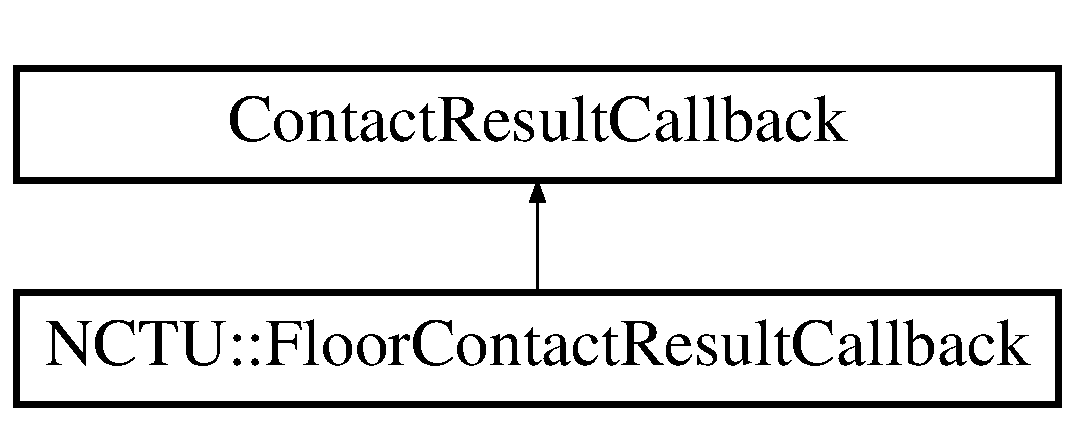
\includegraphics[height=2.000000cm]{struct_n_c_t_u_1_1_floor_contact_result_callback}
\end{center}
\end{figure}
\subsection*{Public Member Functions}
\begin{DoxyCompactItemize}
\item 
\hyperlink{struct_n_c_t_u_1_1_floor_contact_result_callback_a837efd6e0899096a004133dd526084bd}{Floor\+Contact\+Result\+Callback} (\hyperlink{class_n_c_t_u_1_1_obstacle}{Obstacle} $\ast$ptr)\hypertarget{struct_n_c_t_u_1_1_floor_contact_result_callback_a837efd6e0899096a004133dd526084bd}{}\label{struct_n_c_t_u_1_1_floor_contact_result_callback_a837efd6e0899096a004133dd526084bd}

\begin{DoxyCompactList}\small\item\em handle contact result \end{DoxyCompactList}\item 
bt\+Scalar {\bfseries add\+Single\+Result} (bt\+Manifold\+Point \&cp, const bt\+Collision\+Object\+Wrapper $\ast$col\+Obj0\+Wrap, int part\+Id0, int index0, const bt\+Collision\+Object\+Wrapper $\ast$col\+Obj1\+Wrap, int part\+Id1, int index1)\hypertarget{struct_n_c_t_u_1_1_floor_contact_result_callback_af6e9cbd28d3ea79f9719c0d023f9dc09}{}\label{struct_n_c_t_u_1_1_floor_contact_result_callback_af6e9cbd28d3ea79f9719c0d023f9dc09}

\end{DoxyCompactItemize}
\subsection*{Public Attributes}
\begin{DoxyCompactItemize}
\item 
\hyperlink{class_n_c_t_u_1_1_obstacle}{Obstacle} $\ast$ \hyperlink{struct_n_c_t_u_1_1_floor_contact_result_callback_a87b90c0dadbb358e7e3f080adb4202e1}{m\+Subject}\hypertarget{struct_n_c_t_u_1_1_floor_contact_result_callback_a87b90c0dadbb358e7e3f080adb4202e1}{}\label{struct_n_c_t_u_1_1_floor_contact_result_callback_a87b90c0dadbb358e7e3f080adb4202e1}

\begin{DoxyCompactList}\small\item\em pointer to the subject \end{DoxyCompactList}\end{DoxyCompactItemize}


\subsection{Detailed Description}
callback for player-\/floor contact 

The documentation for this struct was generated from the following files\+:\begin{DoxyCompactItemize}
\item 
N\+C\+T\+U\+Obstacle/include/N\+C\+T\+U\+Obstacle\+Callback.\+h\item 
N\+C\+T\+U\+Obstacle/src/N\+C\+T\+U\+Obstacle\+Callback.\+cpp\end{DoxyCompactItemize}

\hypertarget{class_n_c_t_u_1_1_floor_obstacle}{}\section{N\+C\+TU\+:\+:Floor\+Obstacle Class Reference}
\label{class_n_c_t_u_1_1_floor_obstacle}\index{N\+C\+T\+U\+::\+Floor\+Obstacle@{N\+C\+T\+U\+::\+Floor\+Obstacle}}


floor obstacke  




{\ttfamily \#include $<$N\+C\+T\+U\+Floor\+Obstacle.\+h$>$}

Inheritance diagram for N\+C\+TU\+:\+:Floor\+Obstacle\+:\begin{figure}[H]
\begin{center}
\leavevmode
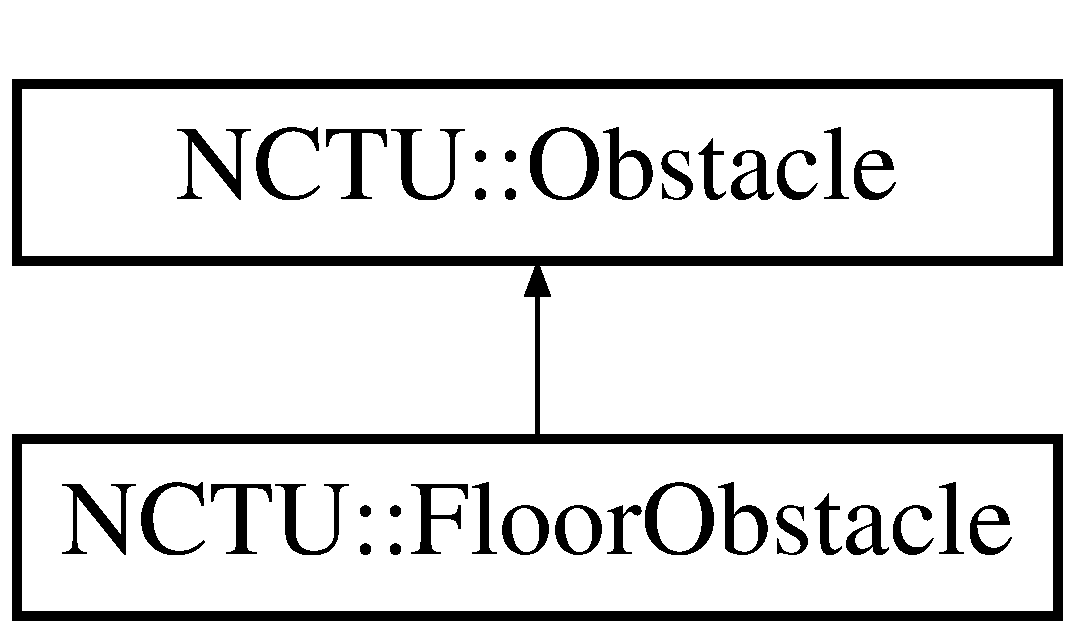
\includegraphics[height=2.000000cm]{class_n_c_t_u_1_1_floor_obstacle}
\end{center}
\end{figure}
\subsection*{Public Member Functions}
\begin{DoxyCompactItemize}
\item 
\hyperlink{class_n_c_t_u_1_1_floor_obstacle_a294bf5268a78caaa328672bfd645150b}{Floor\+Obstacle} (\hyperlink{class_n_c_t_u_1_1_obstacle_manager}{Obstacle\+Manager} $\ast$mgmt, Ogre\+::\+Real restitution, Ogre\+::\+Real friction, const Ogre\+::\+Vector3 \&normal, Ogre\+::\+Real distance)\hypertarget{class_n_c_t_u_1_1_floor_obstacle_a294bf5268a78caaa328672bfd645150b}{}\label{class_n_c_t_u_1_1_floor_obstacle_a294bf5268a78caaa328672bfd645150b}

\begin{DoxyCompactList}\small\item\em constructor \end{DoxyCompactList}\item 
\hyperlink{class_n_c_t_u_1_1_floor_obstacle_abeac4b4c5816079be57518efe2a931e7}{Floor\+Obstacle} (\hyperlink{class_n_c_t_u_1_1_obstacle_manager}{Obstacle\+Manager} $\ast$mgmt, Ogre\+::\+Real restitution, Ogre\+::\+Real friction, Ogre\+::\+Plane \&plane, Ogre\+::\+Entity $\ast$entity)\hypertarget{class_n_c_t_u_1_1_floor_obstacle_abeac4b4c5816079be57518efe2a931e7}{}\label{class_n_c_t_u_1_1_floor_obstacle_abeac4b4c5816079be57518efe2a931e7}

\begin{DoxyCompactList}\small\item\em constructor without creating Ogre3D object \end{DoxyCompactList}\end{DoxyCompactItemize}
\subsection*{Protected Attributes}
\begin{DoxyCompactItemize}
\item 
Ogre\+::\+Vector3 \hyperlink{class_n_c_t_u_1_1_floor_obstacle_a1e67d672c9203daf792e43a02892178f}{m\+Normal}\hypertarget{class_n_c_t_u_1_1_floor_obstacle_a1e67d672c9203daf792e43a02892178f}{}\label{class_n_c_t_u_1_1_floor_obstacle_a1e67d672c9203daf792e43a02892178f}

\begin{DoxyCompactList}\small\item\em plane normal \end{DoxyCompactList}\item 
Ogre\+::\+Real \hyperlink{class_n_c_t_u_1_1_floor_obstacle_a6c9b0351b04062bf40001c66296722e7}{m\+Distance}\hypertarget{class_n_c_t_u_1_1_floor_obstacle_a6c9b0351b04062bf40001c66296722e7}{}\label{class_n_c_t_u_1_1_floor_obstacle_a6c9b0351b04062bf40001c66296722e7}

\begin{DoxyCompactList}\small\item\em plane distance \end{DoxyCompactList}\item 
Ogre\+::\+Plane \hyperlink{class_n_c_t_u_1_1_floor_obstacle_adb824abf9f590ee417acbfd7a4f17aaf}{m\+Plane}\hypertarget{class_n_c_t_u_1_1_floor_obstacle_adb824abf9f590ee417acbfd7a4f17aaf}{}\label{class_n_c_t_u_1_1_floor_obstacle_adb824abf9f590ee417acbfd7a4f17aaf}

\begin{DoxyCompactList}\small\item\em Ogre3D plane object. \end{DoxyCompactList}\end{DoxyCompactItemize}
\subsection*{Additional Inherited Members}


\subsection{Detailed Description}
floor obstacke 

The documentation for this class was generated from the following file\+:\begin{DoxyCompactItemize}
\item 
N\+C\+T\+U\+Obstacle/include/N\+C\+T\+U\+Floor\+Obstacle.\+h\end{DoxyCompactItemize}

\hypertarget{class_n_c_t_u_1_1_game_console_window}{}\section{N\+C\+TU\+:\+:Game\+Console\+Window Class Reference}
\label{class_n_c_t_u_1_1_game_console_window}\index{N\+C\+T\+U\+::\+Game\+Console\+Window@{N\+C\+T\+U\+::\+Game\+Console\+Window}}


G\+UI window fro C\+E\+G\+UI demo, not used in game.  




{\ttfamily \#include $<$Game\+Console\+Window.\+h$>$}

Inheritance diagram for N\+C\+TU\+:\+:Game\+Console\+Window\+:\begin{figure}[H]
\begin{center}
\leavevmode
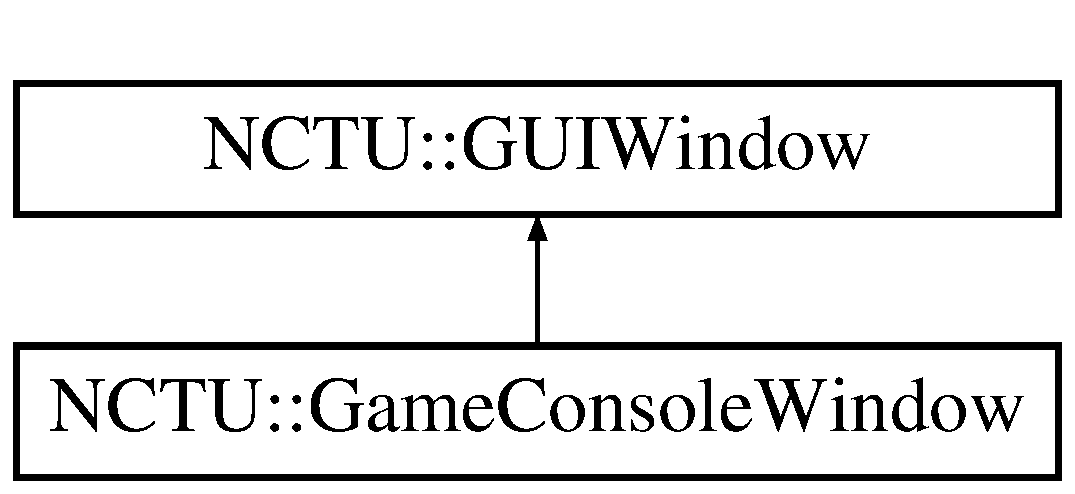
\includegraphics[height=2.000000cm]{class_n_c_t_u_1_1_game_console_window}
\end{center}
\end{figure}
\subsection*{Public Member Functions}
\begin{DoxyCompactItemize}
\item 
\hyperlink{class_n_c_t_u_1_1_game_console_window_a31f18fec374288dfab5e219ea03fe40f}{Game\+Console\+Window} ()\hypertarget{class_n_c_t_u_1_1_game_console_window_a31f18fec374288dfab5e219ea03fe40f}{}\label{class_n_c_t_u_1_1_game_console_window_a31f18fec374288dfab5e219ea03fe40f}

\begin{DoxyCompactList}\small\item\em constructor \end{DoxyCompactList}\end{DoxyCompactItemize}
\subsection*{Protected Member Functions}
\begin{DoxyCompactItemize}
\item 
virtual void \hyperlink{class_n_c_t_u_1_1_game_console_window_a6274ef02dd735e8df10f6d5349d88ddc}{register\+Handlers} ()\hypertarget{class_n_c_t_u_1_1_game_console_window_a6274ef02dd735e8df10f6d5349d88ddc}{}\label{class_n_c_t_u_1_1_game_console_window_a6274ef02dd735e8df10f6d5349d88ddc}

\begin{DoxyCompactList}\small\item\em Register our handler functions. \end{DoxyCompactList}\item 
bool \hyperlink{class_n_c_t_u_1_1_game_console_window_a5b981f9d624d03c1bb265c974b5a6608}{Handle\+\_\+\+Text\+Submitted} (const C\+E\+G\+U\+I\+::\+Event\+Args \&e)\hypertarget{class_n_c_t_u_1_1_game_console_window_a5b981f9d624d03c1bb265c974b5a6608}{}\label{class_n_c_t_u_1_1_game_console_window_a5b981f9d624d03c1bb265c974b5a6608}

\begin{DoxyCompactList}\small\item\em Handle when we press Enter after typing. \end{DoxyCompactList}\item 
bool \hyperlink{class_n_c_t_u_1_1_game_console_window_a373ef277c17527289fc93dac39d95800}{Handle\+\_\+\+Send\+Button\+Pressed} (const C\+E\+G\+U\+I\+::\+Event\+Args \&e)\hypertarget{class_n_c_t_u_1_1_game_console_window_a373ef277c17527289fc93dac39d95800}{}\label{class_n_c_t_u_1_1_game_console_window_a373ef277c17527289fc93dac39d95800}

\begin{DoxyCompactList}\small\item\em Handle when we press the Send button. \end{DoxyCompactList}\item 
void \hyperlink{class_n_c_t_u_1_1_game_console_window_a6518b335a1091432dca37abef7fea6e1}{Parse\+Text} (C\+E\+G\+U\+I\+::\+String in\+Msg)\hypertarget{class_n_c_t_u_1_1_game_console_window_a6518b335a1091432dca37abef7fea6e1}{}\label{class_n_c_t_u_1_1_game_console_window_a6518b335a1091432dca37abef7fea6e1}

\begin{DoxyCompactList}\small\item\em Parse the text the user submitted. \end{DoxyCompactList}\item 
void \hyperlink{class_n_c_t_u_1_1_game_console_window_a2343eb496dd5be2a4bfe2c13d9530069}{Output\+Text} (C\+E\+G\+U\+I\+::\+String in\+Msg, C\+E\+G\+U\+I\+::\+Colour colour=C\+E\+G\+U\+I\+::\+Colour(0x\+F\+F\+F\+F\+F\+F\+F\+F))\hypertarget{class_n_c_t_u_1_1_game_console_window_a2343eb496dd5be2a4bfe2c13d9530069}{}\label{class_n_c_t_u_1_1_game_console_window_a2343eb496dd5be2a4bfe2c13d9530069}

\begin{DoxyCompactList}\small\item\em Post the message to the Chat\+History listbox. \end{DoxyCompactList}\end{DoxyCompactItemize}
\subsection*{Additional Inherited Members}


\subsection{Detailed Description}
G\+UI window fro C\+E\+G\+UI demo, not used in game. 

The documentation for this class was generated from the following files\+:\begin{DoxyCompactItemize}
\item 
programs/\+Obstacle/include/Game\+Console\+Window.\+h\item 
programs/\+Obstacle/source/Game\+Console\+Window.\+cpp\end{DoxyCompactItemize}

\hypertarget{class_n_c_t_u_1_1_game_menu_window}{}\section{N\+C\+TU\+:\+:Game\+Menu\+Window Class Reference}
\label{class_n_c_t_u_1_1_game_menu_window}\index{N\+C\+T\+U\+::\+Game\+Menu\+Window@{N\+C\+T\+U\+::\+Game\+Menu\+Window}}


Menu window.  




{\ttfamily \#include $<$Game\+Menu\+Window.\+h$>$}

Inheritance diagram for N\+C\+TU\+:\+:Game\+Menu\+Window\+:\begin{figure}[H]
\begin{center}
\leavevmode
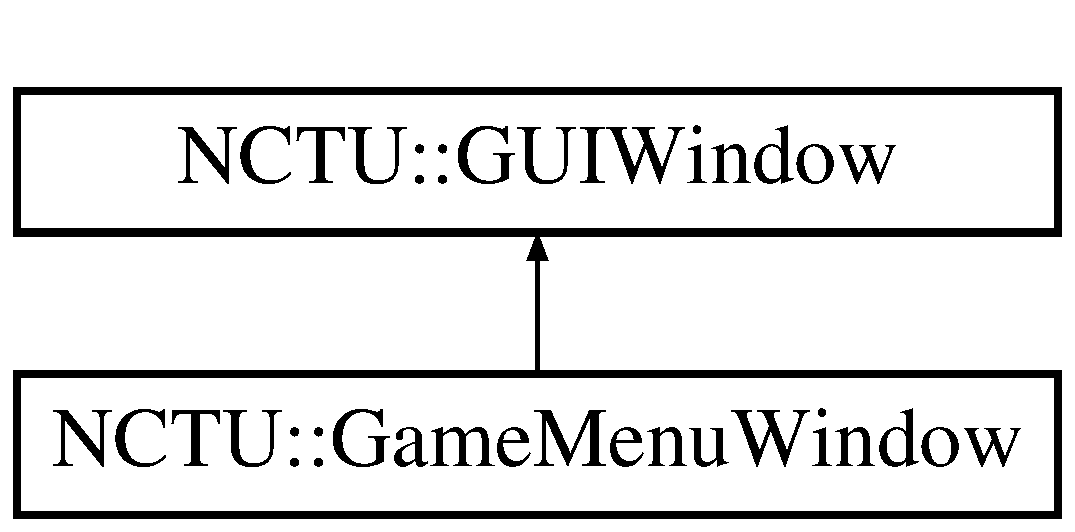
\includegraphics[height=2.000000cm]{class_n_c_t_u_1_1_game_menu_window}
\end{center}
\end{figure}
\subsection*{Public Member Functions}
\begin{DoxyCompactItemize}
\item 
\hyperlink{class_n_c_t_u_1_1_game_menu_window_a5721659b034229cf3154122986bed825}{Game\+Menu\+Window} ()\hypertarget{class_n_c_t_u_1_1_game_menu_window_a5721659b034229cf3154122986bed825}{}\label{class_n_c_t_u_1_1_game_menu_window_a5721659b034229cf3154122986bed825}

\begin{DoxyCompactList}\small\item\em constructor \end{DoxyCompactList}\end{DoxyCompactItemize}
\subsection*{Protected Member Functions}
\begin{DoxyCompactItemize}
\item 
virtual void \hyperlink{class_n_c_t_u_1_1_game_menu_window_accc2e422a42829a2ff7dc6c1d4110436}{register\+Handlers} ()\hypertarget{class_n_c_t_u_1_1_game_menu_window_accc2e422a42829a2ff7dc6c1d4110436}{}\label{class_n_c_t_u_1_1_game_menu_window_accc2e422a42829a2ff7dc6c1d4110436}

\begin{DoxyCompactList}\small\item\em register event handlers \end{DoxyCompactList}\item 
bool \hyperlink{class_n_c_t_u_1_1_game_menu_window_a47e996ebace14a24d335ef9f5223fe1d}{on\+Press\+Resume} (const C\+E\+G\+U\+I\+::\+Event\+Args \&e)\hypertarget{class_n_c_t_u_1_1_game_menu_window_a47e996ebace14a24d335ef9f5223fe1d}{}\label{class_n_c_t_u_1_1_game_menu_window_a47e996ebace14a24d335ef9f5223fe1d}

\begin{DoxyCompactList}\small\item\em process when press resume botton \end{DoxyCompactList}\item 
bool \hyperlink{class_n_c_t_u_1_1_game_menu_window_aaeeccf9f45968a40875537f14b10b3a2}{on\+Press\+Exit} (const C\+E\+G\+U\+I\+::\+Event\+Args \&e)\hypertarget{class_n_c_t_u_1_1_game_menu_window_aaeeccf9f45968a40875537f14b10b3a2}{}\label{class_n_c_t_u_1_1_game_menu_window_aaeeccf9f45968a40875537f14b10b3a2}

\begin{DoxyCompactList}\small\item\em process when press exit botton \end{DoxyCompactList}\item 
bool \hyperlink{class_n_c_t_u_1_1_game_menu_window_a0bf12a3562e057091ea60c21d5199d0a}{on\+Press\+Main\+Menu} (const C\+E\+G\+U\+I\+::\+Event\+Args \&e)\hypertarget{class_n_c_t_u_1_1_game_menu_window_a0bf12a3562e057091ea60c21d5199d0a}{}\label{class_n_c_t_u_1_1_game_menu_window_a0bf12a3562e057091ea60c21d5199d0a}

\begin{DoxyCompactList}\small\item\em process when press Main\+Menu botton \end{DoxyCompactList}\end{DoxyCompactItemize}
\subsection*{Additional Inherited Members}


\subsection{Detailed Description}
Menu window. 

The documentation for this class was generated from the following files\+:\begin{DoxyCompactItemize}
\item 
programs/\+Obstacle/include/Game\+Menu\+Window.\+h\item 
programs/\+Obstacle/source/Game\+Menu\+Window.\+cpp\end{DoxyCompactItemize}

\hypertarget{class_n_c_t_u_1_1_game_over_window}{}\section{N\+C\+TU\+:\+:Game\+Over\+Window Class Reference}
\label{class_n_c_t_u_1_1_game_over_window}\index{N\+C\+T\+U\+::\+Game\+Over\+Window@{N\+C\+T\+U\+::\+Game\+Over\+Window}}


G\+UI window for Game Over.  




{\ttfamily \#include $<$Game\+Over\+Window.\+h$>$}

Inheritance diagram for N\+C\+TU\+:\+:Game\+Over\+Window\+:\begin{figure}[H]
\begin{center}
\leavevmode
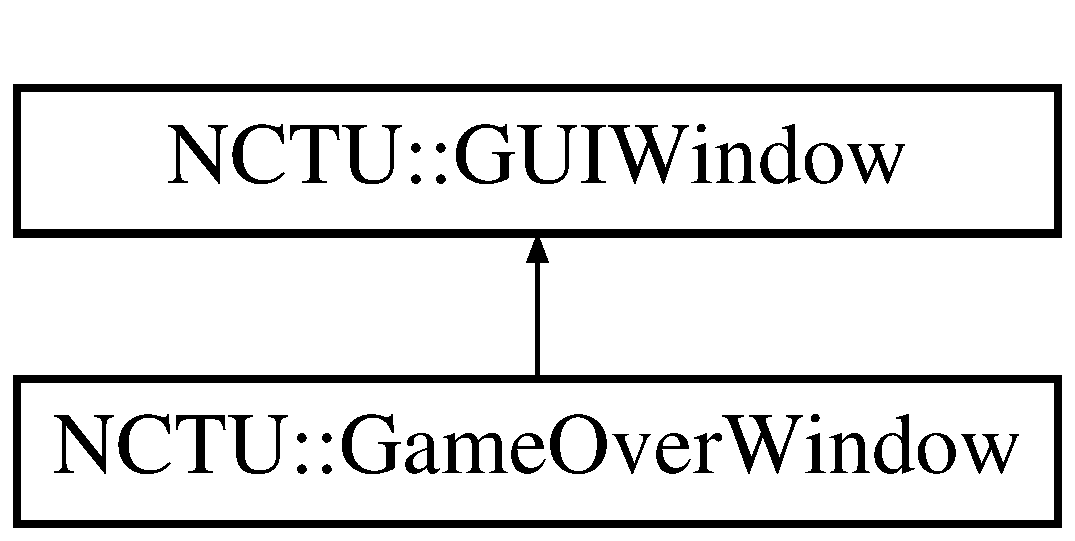
\includegraphics[height=2.000000cm]{class_n_c_t_u_1_1_game_over_window}
\end{center}
\end{figure}
\subsection*{Public Member Functions}
\begin{DoxyCompactItemize}
\item 
\hyperlink{class_n_c_t_u_1_1_game_over_window_a9d321911e4e3ffe1fad77e2ceba5645e}{Game\+Over\+Window} ()\hypertarget{class_n_c_t_u_1_1_game_over_window_a9d321911e4e3ffe1fad77e2ceba5645e}{}\label{class_n_c_t_u_1_1_game_over_window_a9d321911e4e3ffe1fad77e2ceba5645e}

\begin{DoxyCompactList}\small\item\em constructor \end{DoxyCompactList}\end{DoxyCompactItemize}
\subsection*{Protected Member Functions}
\begin{DoxyCompactItemize}
\item 
virtual void \hyperlink{class_n_c_t_u_1_1_game_over_window_aac33006dbd35e83618067e7b8263f098}{register\+Handlers} ()\hypertarget{class_n_c_t_u_1_1_game_over_window_aac33006dbd35e83618067e7b8263f098}{}\label{class_n_c_t_u_1_1_game_over_window_aac33006dbd35e83618067e7b8263f098}

\begin{DoxyCompactList}\small\item\em register event handler \end{DoxyCompactList}\item 
bool \hyperlink{class_n_c_t_u_1_1_game_over_window_ab696a97c72ec421f05ed1fcb553e37ee}{on\+Press\+Exit} (const C\+E\+G\+U\+I\+::\+Event\+Args \&e)\hypertarget{class_n_c_t_u_1_1_game_over_window_ab696a97c72ec421f05ed1fcb553e37ee}{}\label{class_n_c_t_u_1_1_game_over_window_ab696a97c72ec421f05ed1fcb553e37ee}

\begin{DoxyCompactList}\small\item\em process when press exit botton \end{DoxyCompactList}\item 
bool \hyperlink{class_n_c_t_u_1_1_game_over_window_a1eb028d09adc5f6dbbbbec6aa52ac156}{on\+Press\+Main\+Menu} (const C\+E\+G\+U\+I\+::\+Event\+Args \&e)\hypertarget{class_n_c_t_u_1_1_game_over_window_a1eb028d09adc5f6dbbbbec6aa52ac156}{}\label{class_n_c_t_u_1_1_game_over_window_a1eb028d09adc5f6dbbbbec6aa52ac156}

\begin{DoxyCompactList}\small\item\em process when press Main\+Menu botton \end{DoxyCompactList}\end{DoxyCompactItemize}
\subsection*{Additional Inherited Members}


\subsection{Detailed Description}
G\+UI window for Game Over. 

The documentation for this class was generated from the following files\+:\begin{DoxyCompactItemize}
\item 
programs/\+Obstacle/include/Game\+Over\+Window.\+h\item 
programs/\+Obstacle/source/Game\+Over\+Window.\+cpp\end{DoxyCompactItemize}

\hypertarget{class_n_c_t_u_1_1_general_obstacle}{}\section{N\+C\+TU\+:\+:General\+Obstacle Class Reference}
\label{class_n_c_t_u_1_1_general_obstacle}\index{N\+C\+T\+U\+::\+General\+Obstacle@{N\+C\+T\+U\+::\+General\+Obstacle}}


general obstacle  




{\ttfamily \#include $<$N\+C\+T\+U\+General\+Obstacle.\+h$>$}

Inheritance diagram for N\+C\+TU\+:\+:General\+Obstacle\+:\begin{figure}[H]
\begin{center}
\leavevmode
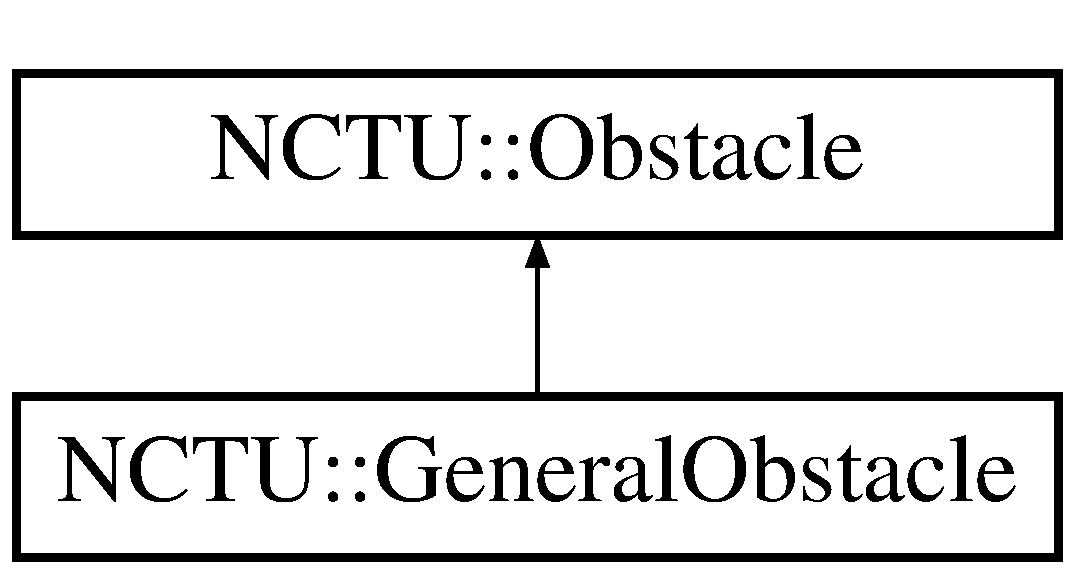
\includegraphics[height=2.000000cm]{class_n_c_t_u_1_1_general_obstacle}
\end{center}
\end{figure}
\subsection*{Public Member Functions}
\begin{DoxyCompactItemize}
\item 
\hyperlink{class_n_c_t_u_1_1_general_obstacle_a470f226cabad51ad2ea342e445507bd4}{General\+Obstacle} (\hyperlink{class_n_c_t_u_1_1_obstacle_manager}{Obstacle\+Manager} $\ast$mgmt, Ogre\+::\+Real restitution, Ogre\+::\+Real friction, Ogre\+::\+Real mass, I\+N\+D\+E\+X\+\_\+\+T\+Y\+PE index, Ogre\+::\+Scene\+Node $\ast$node, Ogre\+::\+Entity $\ast$ent)\hypertarget{class_n_c_t_u_1_1_general_obstacle_a470f226cabad51ad2ea342e445507bd4}{}\label{class_n_c_t_u_1_1_general_obstacle_a470f226cabad51ad2ea342e445507bd4}

\begin{DoxyCompactList}\small\item\em constructor \end{DoxyCompactList}\end{DoxyCompactItemize}
\subsection*{Protected Attributes}
\begin{DoxyCompactItemize}
\item 
I\+N\+D\+E\+X\+\_\+\+T\+Y\+PE \hyperlink{class_n_c_t_u_1_1_general_obstacle_a5fa820e0ed1303f92286d65a83fdc5f5}{m\+Index}\hypertarget{class_n_c_t_u_1_1_general_obstacle_a5fa820e0ed1303f92286d65a83fdc5f5}{}\label{class_n_c_t_u_1_1_general_obstacle_a5fa820e0ed1303f92286d65a83fdc5f5}

\begin{DoxyCompactList}\small\item\em object index \end{DoxyCompactList}\end{DoxyCompactItemize}
\subsection*{Additional Inherited Members}


\subsection{Detailed Description}
general obstacle 

The documentation for this class was generated from the following files\+:\begin{DoxyCompactItemize}
\item 
N\+C\+T\+U\+Obstacle/include/N\+C\+T\+U\+General\+Obstacle.\+h\item 
N\+C\+T\+U\+Obstacle/src/N\+C\+T\+U\+General\+Obstacle.\+cpp\end{DoxyCompactItemize}

\hypertarget{class_ogre_1_1_general_property}{}\section{Ogre\+:\+:General\+Property Class Reference}
\label{class_ogre_1_1_general_property}\index{Ogre\+::\+General\+Property@{Ogre\+::\+General\+Property}}


general property for game  




{\ttfamily \#include $<$Dot\+Scene\+Loader.\+h$>$}

\subsection*{Public Member Functions}
\begin{DoxyCompactItemize}
\item 
\hyperlink{class_ogre_1_1_general_property_acd71b59ffe1f1ce802513435f482175c}{General\+Property} ()\hypertarget{class_ogre_1_1_general_property_acd71b59ffe1f1ce802513435f482175c}{}\label{class_ogre_1_1_general_property_acd71b59ffe1f1ce802513435f482175c}

\begin{DoxyCompactList}\small\item\em constructor \end{DoxyCompactList}\end{DoxyCompactItemize}
\subsection*{Public Attributes}
\begin{DoxyCompactItemize}
\item 
String \hyperlink{class_ogre_1_1_general_property_a3e9138cfd8008b21c7cb5c8a501a0b45}{val\+Str}\hypertarget{class_ogre_1_1_general_property_a3e9138cfd8008b21c7cb5c8a501a0b45}{}\label{class_ogre_1_1_general_property_a3e9138cfd8008b21c7cb5c8a501a0b45}

\begin{DoxyCompactList}\small\item\em string value \end{DoxyCompactList}\item 
int \hyperlink{class_ogre_1_1_general_property_a6ac15b8c8fb3d4b2400e270789738502}{val\+Int}\hypertarget{class_ogre_1_1_general_property_a6ac15b8c8fb3d4b2400e270789738502}{}\label{class_ogre_1_1_general_property_a6ac15b8c8fb3d4b2400e270789738502}

\begin{DoxyCompactList}\small\item\em integer value \end{DoxyCompactList}\item 
Real \hyperlink{class_ogre_1_1_general_property_a565d787d48946ff24b7e3ea8dd26e434}{val\+Float}\hypertarget{class_ogre_1_1_general_property_a565d787d48946ff24b7e3ea8dd26e434}{}\label{class_ogre_1_1_general_property_a565d787d48946ff24b7e3ea8dd26e434}

\begin{DoxyCompactList}\small\item\em floating point number value \end{DoxyCompactList}\item 
bool \hyperlink{class_ogre_1_1_general_property_a0b539cf11887b0c312ac261e5c86b572}{val\+Bool}\hypertarget{class_ogre_1_1_general_property_a0b539cf11887b0c312ac261e5c86b572}{}\label{class_ogre_1_1_general_property_a0b539cf11887b0c312ac261e5c86b572}

\begin{DoxyCompactList}\small\item\em boolean value \end{DoxyCompactList}\item 
Var\+Type \hyperlink{class_ogre_1_1_general_property_aa961cf3f31323ed235856a91d1b5e30a}{val\+Type}\hypertarget{class_ogre_1_1_general_property_aa961cf3f31323ed235856a91d1b5e30a}{}\label{class_ogre_1_1_general_property_aa961cf3f31323ed235856a91d1b5e30a}

\begin{DoxyCompactList}\small\item\em value type \end{DoxyCompactList}\end{DoxyCompactItemize}


\subsection{Detailed Description}
general property for game 

The documentation for this class was generated from the following file\+:\begin{DoxyCompactItemize}
\item 
programs/\+Obstacle/include/Dot\+Scene\+Loader.\+h\end{DoxyCompactItemize}

\hypertarget{class_n_c_t_u_1_1_g_u_i_manager}{}\section{N\+C\+TU\+:\+:G\+U\+I\+Manager Class Reference}
\label{class_n_c_t_u_1_1_g_u_i_manager}\index{N\+C\+T\+U\+::\+G\+U\+I\+Manager@{N\+C\+T\+U\+::\+G\+U\+I\+Manager}}


manager class for G\+UI windows  




{\ttfamily \#include $<$N\+C\+T\+U\+G\+U\+I\+Manager.\+h$>$}

\subsection*{Public Member Functions}
\begin{DoxyCompactItemize}
\item 
\hyperlink{class_n_c_t_u_1_1_g_u_i_manager_a5587062fc64af58b9adbe5df4ba25097}{G\+U\+I\+Manager} ()\hypertarget{class_n_c_t_u_1_1_g_u_i_manager_a5587062fc64af58b9adbe5df4ba25097}{}\label{class_n_c_t_u_1_1_g_u_i_manager_a5587062fc64af58b9adbe5df4ba25097}

\begin{DoxyCompactList}\small\item\em constructor \end{DoxyCompactList}\item 
\hyperlink{class_n_c_t_u_1_1_g_u_i_manager_a4e1a7873e94f406c1b6cb4c50d3f2aab}{$\sim$\+G\+U\+I\+Manager} ()\hypertarget{class_n_c_t_u_1_1_g_u_i_manager_a4e1a7873e94f406c1b6cb4c50d3f2aab}{}\label{class_n_c_t_u_1_1_g_u_i_manager_a4e1a7873e94f406c1b6cb4c50d3f2aab}

\begin{DoxyCompactList}\small\item\em destructor \end{DoxyCompactList}\item 
void \hyperlink{class_n_c_t_u_1_1_g_u_i_manager_a443005af7f4d4e48773e3ddfb823fed1}{setup} (\hyperlink{class_basic_tutorial__00}{Basic\+Tutorial\+\_\+00} $\ast$app)\hypertarget{class_n_c_t_u_1_1_g_u_i_manager_a443005af7f4d4e48773e3ddfb823fed1}{}\label{class_n_c_t_u_1_1_g_u_i_manager_a443005af7f4d4e48773e3ddfb823fed1}

\begin{DoxyCompactList}\small\item\em bind application in the manager \end{DoxyCompactList}\item 
void \hyperlink{class_n_c_t_u_1_1_g_u_i_manager_ab081a5ea774dd9a2cc7cc0ecc809573f}{create\+All\+Window} ()\hypertarget{class_n_c_t_u_1_1_g_u_i_manager_ab081a5ea774dd9a2cc7cc0ecc809573f}{}\label{class_n_c_t_u_1_1_g_u_i_manager_ab081a5ea774dd9a2cc7cc0ecc809573f}

\begin{DoxyCompactList}\small\item\em create all window \end{DoxyCompactList}\item 
void \hyperlink{class_n_c_t_u_1_1_g_u_i_manager_aac5969837735163f0675a9573bce1517}{create\+Console} ()\hypertarget{class_n_c_t_u_1_1_g_u_i_manager_aac5969837735163f0675a9573bce1517}{}\label{class_n_c_t_u_1_1_g_u_i_manager_aac5969837735163f0675a9573bce1517}

\begin{DoxyCompactList}\small\item\em create console window \end{DoxyCompactList}\item 
void \hyperlink{class_n_c_t_u_1_1_g_u_i_manager_a4fc262aae03e436fa639cef515ec153e}{create\+Main\+Menu} ()\hypertarget{class_n_c_t_u_1_1_g_u_i_manager_a4fc262aae03e436fa639cef515ec153e}{}\label{class_n_c_t_u_1_1_g_u_i_manager_a4fc262aae03e436fa639cef515ec153e}

\begin{DoxyCompactList}\small\item\em create main menu window \end{DoxyCompactList}\item 
void \hyperlink{class_n_c_t_u_1_1_g_u_i_manager_a725e1c465b077557a2e3719704e4d42f}{create\+Level\+Menu} ()\hypertarget{class_n_c_t_u_1_1_g_u_i_manager_a725e1c465b077557a2e3719704e4d42f}{}\label{class_n_c_t_u_1_1_g_u_i_manager_a725e1c465b077557a2e3719704e4d42f}

\begin{DoxyCompactList}\small\item\em create level selection window \end{DoxyCompactList}\item 
void \hyperlink{class_n_c_t_u_1_1_g_u_i_manager_ae04e3c736991587a84b8ad635e77f8e9}{create\+Game\+Menu} ()\hypertarget{class_n_c_t_u_1_1_g_u_i_manager_ae04e3c736991587a84b8ad635e77f8e9}{}\label{class_n_c_t_u_1_1_g_u_i_manager_ae04e3c736991587a84b8ad635e77f8e9}

\begin{DoxyCompactList}\small\item\em create game menu for playing game window \end{DoxyCompactList}\item 
void \hyperlink{class_n_c_t_u_1_1_g_u_i_manager_a6550cb1085c935d9128461b73761319e}{create\+Score\+Bar} ()\hypertarget{class_n_c_t_u_1_1_g_u_i_manager_a6550cb1085c935d9128461b73761319e}{}\label{class_n_c_t_u_1_1_g_u_i_manager_a6550cb1085c935d9128461b73761319e}

\begin{DoxyCompactList}\small\item\em create score bar window \end{DoxyCompactList}\item 
void \hyperlink{class_n_c_t_u_1_1_g_u_i_manager_a62f0a4027d39b623ed4cc765e884a88a}{create\+Game\+Over} ()\hypertarget{class_n_c_t_u_1_1_g_u_i_manager_a62f0a4027d39b623ed4cc765e884a88a}{}\label{class_n_c_t_u_1_1_g_u_i_manager_a62f0a4027d39b623ed4cc765e884a88a}

\begin{DoxyCompactList}\small\item\em create game over menu window \end{DoxyCompactList}\item 
void \hyperlink{class_n_c_t_u_1_1_g_u_i_manager_adf56d01be5e9a6c7e8fc13d193a5557a}{update} (double timestep)\hypertarget{class_n_c_t_u_1_1_g_u_i_manager_adf56d01be5e9a6c7e8fc13d193a5557a}{}\label{class_n_c_t_u_1_1_g_u_i_manager_adf56d01be5e9a6c7e8fc13d193a5557a}

\begin{DoxyCompactList}\small\item\em update the manager \end{DoxyCompactList}\item 
bool {\bfseries key\+Pressed} (const O\+I\+S\+::\+Key\+Event \&arg)\hypertarget{class_n_c_t_u_1_1_g_u_i_manager_a3099cc80b76fa94b31fe0469188e7e99}{}\label{class_n_c_t_u_1_1_g_u_i_manager_a3099cc80b76fa94b31fe0469188e7e99}

\item 
bool {\bfseries key\+Released} (const O\+I\+S\+::\+Key\+Event \&arg)\hypertarget{class_n_c_t_u_1_1_g_u_i_manager_afa2eb93ecd6bd394ebbc5394f9036f4f}{}\label{class_n_c_t_u_1_1_g_u_i_manager_afa2eb93ecd6bd394ebbc5394f9036f4f}

\item 
bool {\bfseries mouse\+Moved} (const O\+I\+S\+::\+Mouse\+Event \&arg)\hypertarget{class_n_c_t_u_1_1_g_u_i_manager_a9318f4168f050acfe12406b5595d8c9a}{}\label{class_n_c_t_u_1_1_g_u_i_manager_a9318f4168f050acfe12406b5595d8c9a}

\item 
bool {\bfseries mouse\+Pressed} (const O\+I\+S\+::\+Mouse\+Event \&arg, O\+I\+S\+::\+Mouse\+Button\+ID id)\hypertarget{class_n_c_t_u_1_1_g_u_i_manager_a9960bf4f629c351066197bc15f0eeb87}{}\label{class_n_c_t_u_1_1_g_u_i_manager_a9960bf4f629c351066197bc15f0eeb87}

\item 
bool {\bfseries mouse\+Released} (const O\+I\+S\+::\+Mouse\+Event \&arg, O\+I\+S\+::\+Mouse\+Button\+ID id)\hypertarget{class_n_c_t_u_1_1_g_u_i_manager_a727096747830570784a970bba633c9d8}{}\label{class_n_c_t_u_1_1_g_u_i_manager_a727096747830570784a970bba633c9d8}

\item 
\hyperlink{class_n_c_t_u_1_1_main_menu_window}{Main\+Menu\+Window} $\ast$ \hyperlink{class_n_c_t_u_1_1_g_u_i_manager_ae64dfe5a682d9f26596230234670506c}{get\+Main\+Menu} ()\hypertarget{class_n_c_t_u_1_1_g_u_i_manager_ae64dfe5a682d9f26596230234670506c}{}\label{class_n_c_t_u_1_1_g_u_i_manager_ae64dfe5a682d9f26596230234670506c}

\begin{DoxyCompactList}\small\item\em get pointer of main menu \end{DoxyCompactList}\item 
\hyperlink{class_n_c_t_u_1_1_level_menu_window}{Level\+Menu\+Window} $\ast$ \hyperlink{class_n_c_t_u_1_1_g_u_i_manager_a3126ee946ff53fd489c5ed8da309329e}{get\+Level\+Menu} ()\hypertarget{class_n_c_t_u_1_1_g_u_i_manager_a3126ee946ff53fd489c5ed8da309329e}{}\label{class_n_c_t_u_1_1_g_u_i_manager_a3126ee946ff53fd489c5ed8da309329e}

\begin{DoxyCompactList}\small\item\em get pointer of level menu \end{DoxyCompactList}\item 
\hyperlink{class_n_c_t_u_1_1_game_menu_window}{Game\+Menu\+Window} $\ast$ \hyperlink{class_n_c_t_u_1_1_g_u_i_manager_aff31a9d05ca9682493593d5c03114d3d}{get\+Game\+Menu} ()\hypertarget{class_n_c_t_u_1_1_g_u_i_manager_aff31a9d05ca9682493593d5c03114d3d}{}\label{class_n_c_t_u_1_1_g_u_i_manager_aff31a9d05ca9682493593d5c03114d3d}

\begin{DoxyCompactList}\small\item\em get pointer of game menu \end{DoxyCompactList}\item 
\hyperlink{class_n_c_t_u_1_1_score_bar_window}{Score\+Bar\+Window} $\ast$ \hyperlink{class_n_c_t_u_1_1_g_u_i_manager_aff1ff0c48358b81f1dabc22aa2ce35ab}{get\+Score\+Bar} ()\hypertarget{class_n_c_t_u_1_1_g_u_i_manager_aff1ff0c48358b81f1dabc22aa2ce35ab}{}\label{class_n_c_t_u_1_1_g_u_i_manager_aff1ff0c48358b81f1dabc22aa2ce35ab}

\begin{DoxyCompactList}\small\item\em get pointer of score bar \end{DoxyCompactList}\item 
\hyperlink{class_n_c_t_u_1_1_game_over_window}{Game\+Over\+Window} $\ast$ \hyperlink{class_n_c_t_u_1_1_g_u_i_manager_ae216eab88c6996c84187a5c9b08e3c17}{get\+Game\+Over} ()\hypertarget{class_n_c_t_u_1_1_g_u_i_manager_ae216eab88c6996c84187a5c9b08e3c17}{}\label{class_n_c_t_u_1_1_g_u_i_manager_ae216eab88c6996c84187a5c9b08e3c17}

\begin{DoxyCompactList}\small\item\em get pointer of game over menu \end{DoxyCompactList}\end{DoxyCompactItemize}
\subsection*{Protected Member Functions}
\begin{DoxyCompactItemize}
\item 
C\+E\+G\+U\+I\+::\+Mouse\+Button \hyperlink{class_n_c_t_u_1_1_g_u_i_manager_a18903a21874b5ffd27fa39980f85cf31}{convert\+Button} (O\+I\+S\+::\+Mouse\+Button\+ID button\+ID)\hypertarget{class_n_c_t_u_1_1_g_u_i_manager_a18903a21874b5ffd27fa39980f85cf31}{}\label{class_n_c_t_u_1_1_g_u_i_manager_a18903a21874b5ffd27fa39980f85cf31}

\begin{DoxyCompactList}\small\item\em convert O\+IS button data into C\+E\+G\+UI\textquotesingle{}s \end{DoxyCompactList}\end{DoxyCompactItemize}
\subsection*{Protected Attributes}
\begin{DoxyCompactItemize}
\item 
C\+E\+G\+U\+I\+::\+Ogre\+Renderer $\ast$ \hyperlink{class_n_c_t_u_1_1_g_u_i_manager_adf6b942e5fa01c50f5504f394f006399}{m\+Renderer}\hypertarget{class_n_c_t_u_1_1_g_u_i_manager_adf6b942e5fa01c50f5504f394f006399}{}\label{class_n_c_t_u_1_1_g_u_i_manager_adf6b942e5fa01c50f5504f394f006399}

\begin{DoxyCompactList}\small\item\em the pointer to the C\+E\+G\+U\+I-\/\+Ogre renderer \end{DoxyCompactList}\item 
\hyperlink{class_n_c_t_u_1_1_game_console_window}{Game\+Console\+Window} $\ast$ \hyperlink{class_n_c_t_u_1_1_g_u_i_manager_ae1bb959fda0b357fd87da17db29fc0b5}{m\+Console}\hypertarget{class_n_c_t_u_1_1_g_u_i_manager_ae1bb959fda0b357fd87da17db29fc0b5}{}\label{class_n_c_t_u_1_1_g_u_i_manager_ae1bb959fda0b357fd87da17db29fc0b5}

\begin{DoxyCompactList}\small\item\em the demo console window \end{DoxyCompactList}\item 
\hyperlink{class_n_c_t_u_1_1_main_menu_window}{Main\+Menu\+Window} $\ast$ \hyperlink{class_n_c_t_u_1_1_g_u_i_manager_ad88e4d041ef71c9a74133eebda7439ef}{m\+Main\+Menu}\hypertarget{class_n_c_t_u_1_1_g_u_i_manager_ad88e4d041ef71c9a74133eebda7439ef}{}\label{class_n_c_t_u_1_1_g_u_i_manager_ad88e4d041ef71c9a74133eebda7439ef}

\begin{DoxyCompactList}\small\item\em the main menu window \end{DoxyCompactList}\item 
\hyperlink{class_n_c_t_u_1_1_level_menu_window}{Level\+Menu\+Window} $\ast$ \hyperlink{class_n_c_t_u_1_1_g_u_i_manager_abdd3d8ca1fcf2653ddd35ed0ec3bd195}{m\+Level\+Menu}\hypertarget{class_n_c_t_u_1_1_g_u_i_manager_abdd3d8ca1fcf2653ddd35ed0ec3bd195}{}\label{class_n_c_t_u_1_1_g_u_i_manager_abdd3d8ca1fcf2653ddd35ed0ec3bd195}

\begin{DoxyCompactList}\small\item\em the level selection menu window \end{DoxyCompactList}\item 
\hyperlink{class_n_c_t_u_1_1_game_menu_window}{Game\+Menu\+Window} $\ast$ \hyperlink{class_n_c_t_u_1_1_g_u_i_manager_a0443c02168d031c5ac6f4caecb426ed9}{m\+Game\+Menu}\hypertarget{class_n_c_t_u_1_1_g_u_i_manager_a0443c02168d031c5ac6f4caecb426ed9}{}\label{class_n_c_t_u_1_1_g_u_i_manager_a0443c02168d031c5ac6f4caecb426ed9}

\begin{DoxyCompactList}\small\item\em the game menu window \end{DoxyCompactList}\item 
\hyperlink{class_n_c_t_u_1_1_game_over_window}{Game\+Over\+Window} $\ast$ \hyperlink{class_n_c_t_u_1_1_g_u_i_manager_a68d462d40647f785234e7d77d4c8229d}{m\+Game\+Over}\hypertarget{class_n_c_t_u_1_1_g_u_i_manager_a68d462d40647f785234e7d77d4c8229d}{}\label{class_n_c_t_u_1_1_g_u_i_manager_a68d462d40647f785234e7d77d4c8229d}

\begin{DoxyCompactList}\small\item\em the game over window \end{DoxyCompactList}\item 
\hyperlink{class_n_c_t_u_1_1_score_bar_window}{Score\+Bar\+Window} $\ast$ \hyperlink{class_n_c_t_u_1_1_g_u_i_manager_aea42b1af9d6b26dab0c8969d5718a63d}{m\+Score\+Bar}\hypertarget{class_n_c_t_u_1_1_g_u_i_manager_aea42b1af9d6b26dab0c8969d5718a63d}{}\label{class_n_c_t_u_1_1_g_u_i_manager_aea42b1af9d6b26dab0c8969d5718a63d}

\begin{DoxyCompactList}\small\item\em the score bar window \end{DoxyCompactList}\item 
\hyperlink{class_basic_tutorial__00}{Basic\+Tutorial\+\_\+00} $\ast$ \hyperlink{class_n_c_t_u_1_1_g_u_i_manager_a8271d8105e254bda58752cf35a4d28fa}{m\+App}\hypertarget{class_n_c_t_u_1_1_g_u_i_manager_a8271d8105e254bda58752cf35a4d28fa}{}\label{class_n_c_t_u_1_1_g_u_i_manager_a8271d8105e254bda58752cf35a4d28fa}

\begin{DoxyCompactList}\small\item\em pointer to the Application \end{DoxyCompactList}\end{DoxyCompactItemize}


\subsection{Detailed Description}
manager class for G\+UI windows 

The documentation for this class was generated from the following files\+:\begin{DoxyCompactItemize}
\item 
programs/\+Obstacle/include/N\+C\+T\+U\+G\+U\+I\+Manager.\+h\item 
programs/\+Obstacle/source/N\+C\+T\+U\+G\+U\+I\+Manager.\+cpp\end{DoxyCompactItemize}

\hypertarget{class_n_c_t_u_1_1_g_u_i_window}{}\section{N\+C\+TU\+:\+:G\+U\+I\+Window Class Reference}
\label{class_n_c_t_u_1_1_g_u_i_window}\index{N\+C\+T\+U\+::\+G\+U\+I\+Window@{N\+C\+T\+U\+::\+G\+U\+I\+Window}}


base class for all G\+UI window in this project  




{\ttfamily \#include $<$N\+C\+T\+U\+G\+U\+I\+Window.\+h$>$}

Inheritance diagram for N\+C\+TU\+:\+:G\+U\+I\+Window\+:\begin{figure}[H]
\begin{center}
\leavevmode
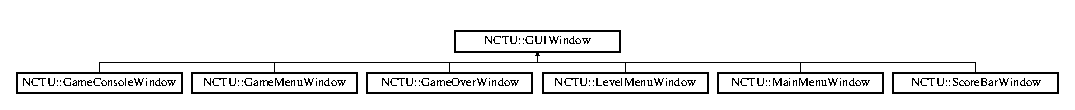
\includegraphics[height=1.031308cm]{class_n_c_t_u_1_1_g_u_i_window}
\end{center}
\end{figure}
\subsection*{Public Member Functions}
\begin{DoxyCompactItemize}
\item 
\hyperlink{class_n_c_t_u_1_1_g_u_i_window_a17117dcf2c77d559f55667e141f7ca15}{G\+U\+I\+Window} (const C\+E\+G\+U\+I\+::\+String \&layout)\hypertarget{class_n_c_t_u_1_1_g_u_i_window_a17117dcf2c77d559f55667e141f7ca15}{}\label{class_n_c_t_u_1_1_g_u_i_window_a17117dcf2c77d559f55667e141f7ca15}

\begin{DoxyCompactList}\small\item\em constructor \end{DoxyCompactList}\item 
virtual \hyperlink{class_n_c_t_u_1_1_g_u_i_window_a9c6d4277ffc74763b0a19fcdf15a5b7c}{$\sim$\+G\+U\+I\+Window} ()\hypertarget{class_n_c_t_u_1_1_g_u_i_window_a9c6d4277ffc74763b0a19fcdf15a5b7c}{}\label{class_n_c_t_u_1_1_g_u_i_window_a9c6d4277ffc74763b0a19fcdf15a5b7c}

\begin{DoxyCompactList}\small\item\em destructor \end{DoxyCompactList}\item 
virtual void \hyperlink{class_n_c_t_u_1_1_g_u_i_window_acbb70d27b61444db31c8e27cab84f1fa}{setup} ()\hypertarget{class_n_c_t_u_1_1_g_u_i_window_acbb70d27b61444db31c8e27cab84f1fa}{}\label{class_n_c_t_u_1_1_g_u_i_window_acbb70d27b61444db31c8e27cab84f1fa}

\begin{DoxyCompactList}\small\item\em setup everything \end{DoxyCompactList}\item 
virtual void \hyperlink{class_n_c_t_u_1_1_g_u_i_window_a2b43d1bd60453002b592dd509b0eb2da}{set\+Visible} (bool visible)\hypertarget{class_n_c_t_u_1_1_g_u_i_window_a2b43d1bd60453002b592dd509b0eb2da}{}\label{class_n_c_t_u_1_1_g_u_i_window_a2b43d1bd60453002b592dd509b0eb2da}

\begin{DoxyCompactList}\small\item\em Hide or show the window. \end{DoxyCompactList}\item 
virtual bool \hyperlink{class_n_c_t_u_1_1_g_u_i_window_a657b0f27eddefc6925f0f8bb5e2fa662}{is\+Visible} ()\hypertarget{class_n_c_t_u_1_1_g_u_i_window_a657b0f27eddefc6925f0f8bb5e2fa662}{}\label{class_n_c_t_u_1_1_g_u_i_window_a657b0f27eddefc6925f0f8bb5e2fa662}

\begin{DoxyCompactList}\small\item\em return true if console is visible, false if is hidden \end{DoxyCompactList}\item 
virtual void \hyperlink{class_n_c_t_u_1_1_g_u_i_window_a94b78a60cc24592db3620bb92577ec6b}{set\+App} (\hyperlink{class_basic_tutorial__00}{Basic\+Tutorial\+\_\+00} $\ast$app)\hypertarget{class_n_c_t_u_1_1_g_u_i_window_a94b78a60cc24592db3620bb92577ec6b}{}\label{class_n_c_t_u_1_1_g_u_i_window_a94b78a60cc24592db3620bb92577ec6b}

\begin{DoxyCompactList}\small\item\em set up application pointer \end{DoxyCompactList}\end{DoxyCompactItemize}
\subsection*{Protected Member Functions}
\begin{DoxyCompactItemize}
\item 
virtual void \hyperlink{class_n_c_t_u_1_1_g_u_i_window_a629179c96d0e8f4cad0c967a5878188e}{create\+C\+E\+G\+U\+I\+Window} ()
\item 
virtual void \hyperlink{class_n_c_t_u_1_1_g_u_i_window_a42122d8c814dd42386a63f14dd91fd02}{register\+Handlers} ()\hypertarget{class_n_c_t_u_1_1_g_u_i_window_a42122d8c814dd42386a63f14dd91fd02}{}\label{class_n_c_t_u_1_1_g_u_i_window_a42122d8c814dd42386a63f14dd91fd02}

\begin{DoxyCompactList}\small\item\em Register our handler functions. \end{DoxyCompactList}\end{DoxyCompactItemize}
\subsection*{Protected Attributes}
\begin{DoxyCompactItemize}
\item 
C\+E\+G\+U\+I\+::\+Window $\ast$ \hyperlink{class_n_c_t_u_1_1_g_u_i_window_a163e8089c4b71d29851ccc155bb81c14}{m\+Window}\hypertarget{class_n_c_t_u_1_1_g_u_i_window_a163e8089c4b71d29851ccc155bb81c14}{}\label{class_n_c_t_u_1_1_g_u_i_window_a163e8089c4b71d29851ccc155bb81c14}

\begin{DoxyCompactList}\small\item\em This will be a pointer to the C\+E\+G\+UI window. \end{DoxyCompactList}\item 
C\+E\+G\+U\+I\+::\+String \hyperlink{class_n_c_t_u_1_1_g_u_i_window_a3335697525abec4a6867f5a2d0b4cb60}{m\+Layout\+Name}\hypertarget{class_n_c_t_u_1_1_g_u_i_window_a3335697525abec4a6867f5a2d0b4cb60}{}\label{class_n_c_t_u_1_1_g_u_i_window_a3335697525abec4a6867f5a2d0b4cb60}

\begin{DoxyCompactList}\small\item\em Store the layout name. \end{DoxyCompactList}\item 
\hyperlink{class_basic_tutorial__00}{Basic\+Tutorial\+\_\+00} $\ast$ \hyperlink{class_n_c_t_u_1_1_g_u_i_window_a81091ea09d7efcc472878fcb6c774e7a}{m\+App}\hypertarget{class_n_c_t_u_1_1_g_u_i_window_a81091ea09d7efcc472878fcb6c774e7a}{}\label{class_n_c_t_u_1_1_g_u_i_window_a81091ea09d7efcc472878fcb6c774e7a}

\begin{DoxyCompactList}\small\item\em pointer to the application \end{DoxyCompactList}\end{DoxyCompactItemize}


\subsection{Detailed Description}
base class for all G\+UI window in this project 

\subsection{Member Function Documentation}
\index{N\+C\+T\+U\+::\+G\+U\+I\+Window@{N\+C\+T\+U\+::\+G\+U\+I\+Window}!create\+C\+E\+G\+U\+I\+Window@{create\+C\+E\+G\+U\+I\+Window}}
\index{create\+C\+E\+G\+U\+I\+Window@{create\+C\+E\+G\+U\+I\+Window}!N\+C\+T\+U\+::\+G\+U\+I\+Window@{N\+C\+T\+U\+::\+G\+U\+I\+Window}}
\subsubsection[{\texorpdfstring{create\+C\+E\+G\+U\+I\+Window()}{createCEGUIWindow()}}]{\setlength{\rightskip}{0pt plus 5cm}void G\+U\+I\+Window\+::create\+C\+E\+G\+U\+I\+Window (
\begin{DoxyParamCaption}
{}
\end{DoxyParamCaption}
)\hspace{0.3cm}{\ttfamily [protected]}, {\ttfamily [virtual]}}\hypertarget{class_n_c_t_u_1_1_g_u_i_window_a629179c96d0e8f4cad0c967a5878188e}{}\label{class_n_c_t_u_1_1_g_u_i_window_a629179c96d0e8f4cad0c967a5878188e}
The function which will load in the C\+E\+G\+UI Window and register event handlers 

The documentation for this class was generated from the following files\+:\begin{DoxyCompactItemize}
\item 
programs/\+Obstacle/include/N\+C\+T\+U\+G\+U\+I\+Window.\+h\item 
programs/\+Obstacle/source/N\+C\+T\+U\+G\+U\+I\+Window.\+cpp\end{DoxyCompactItemize}

\hypertarget{class_key_board_handler}{}\section{Key\+Board\+Handler Class Reference}
\label{class_key_board_handler}\index{Key\+Board\+Handler@{Key\+Board\+Handler}}


keyboard handler class  




{\ttfamily \#include $<$Key\+Board\+Handler.\+h$>$}

\subsection*{Public Member Functions}
\begin{DoxyCompactItemize}
\item 
\hyperlink{class_key_board_handler_a46fad223915367625a9a6ea520840ea6}{Key\+Board\+Handler} (void)\hypertarget{class_key_board_handler_a46fad223915367625a9a6ea520840ea6}{}\label{class_key_board_handler_a46fad223915367625a9a6ea520840ea6}

\begin{DoxyCompactList}\small\item\em constructor \end{DoxyCompactList}\item 
\hyperlink{class_key_board_handler_a614e8a85e534690667be4a9f12bcae02}{$\sim$\+Key\+Board\+Handler} (void)\hypertarget{class_key_board_handler_a614e8a85e534690667be4a9f12bcae02}{}\label{class_key_board_handler_a614e8a85e534690667be4a9f12bcae02}

\begin{DoxyCompactList}\small\item\em destructor \end{DoxyCompactList}\item 
bool \hyperlink{class_key_board_handler_a36fc47555cdfcd33a112a42fc797e620}{is\+Key\+Pressing} (const unsigned char key)\hypertarget{class_key_board_handler_a36fc47555cdfcd33a112a42fc797e620}{}\label{class_key_board_handler_a36fc47555cdfcd33a112a42fc797e620}

\begin{DoxyCompactList}\small\item\em check if a key is pressed? \end{DoxyCompactList}\item 
bool \hyperlink{class_key_board_handler_aeda4d8cbf4f2269fc78e0daa90e5c4ea}{is\+Key\+Triggered} (const unsigned char key)\hypertarget{class_key_board_handler_aeda4d8cbf4f2269fc78e0daa90e5c4ea}{}\label{class_key_board_handler_aeda4d8cbf4f2269fc78e0daa90e5c4ea}

\begin{DoxyCompactList}\small\item\em check if a key is triggered? \end{DoxyCompactList}\item 
bool \hyperlink{class_key_board_handler_ac34388fcd867aac71556626b307a4a6a}{is\+Key\+Pressed\+Long} (const unsigned char key, float time=1.\+0)\hypertarget{class_key_board_handler_ac34388fcd867aac71556626b307a4a6a}{}\label{class_key_board_handler_ac34388fcd867aac71556626b307a4a6a}

\begin{DoxyCompactList}\small\item\em check if a key is pressed for a long time? \end{DoxyCompactList}\item 
bool \hyperlink{class_key_board_handler_a47e6d7e17b07ce2c8b422be62331997e}{is\+Key\+Entered} (const unsigned char key)\hypertarget{class_key_board_handler_a47e6d7e17b07ce2c8b422be62331997e}{}\label{class_key_board_handler_a47e6d7e17b07ce2c8b422be62331997e}

\begin{DoxyCompactList}\small\item\em check if a key is entered? \end{DoxyCompactList}\item 
void \hyperlink{class_key_board_handler_a188044605994c92b1a1bed5f3d1137f7}{key\+Pressed} (const O\+I\+S\+::\+Key\+Event \&arg)\hypertarget{class_key_board_handler_a188044605994c92b1a1bed5f3d1137f7}{}\label{class_key_board_handler_a188044605994c92b1a1bed5f3d1137f7}

\begin{DoxyCompactList}\small\item\em handler for O\+IS key\+Presssed \end{DoxyCompactList}\item 
void \hyperlink{class_key_board_handler_ac32dcdc6731d458aa8f557e723ed9d5f}{key\+Released} (const O\+I\+S\+::\+Key\+Event \&arg)\hypertarget{class_key_board_handler_ac32dcdc6731d458aa8f557e723ed9d5f}{}\label{class_key_board_handler_ac32dcdc6731d458aa8f557e723ed9d5f}

\begin{DoxyCompactList}\small\item\em handler fir O\+IS key\+Released \end{DoxyCompactList}\item 
void \hyperlink{class_key_board_handler_a89ccbbf5404145cadec192a0f044b34d}{update\+Data} ()\hypertarget{class_key_board_handler_a89ccbbf5404145cadec192a0f044b34d}{}\label{class_key_board_handler_a89ccbbf5404145cadec192a0f044b34d}

\begin{DoxyCompactList}\small\item\em update the handler \end{DoxyCompactList}\end{DoxyCompactItemize}


\subsection{Detailed Description}
keyboard handler class 

The documentation for this class was generated from the following files\+:\begin{DoxyCompactItemize}
\item 
programs/\+Obstacle/include/Key\+Board\+Handler.\+h\item 
programs/\+Obstacle/source/Key\+Board\+Handler.\+cpp\end{DoxyCompactItemize}

\hypertarget{struct_key_data}{}\section{Key\+Data Struct Reference}
\label{struct_key_data}\index{Key\+Data@{Key\+Data}}


store complete key-\/press data  




{\ttfamily \#include $<$Key\+Board\+Handler.\+h$>$}

\subsection*{Public Attributes}
\begin{DoxyCompactItemize}
\item 
bool {\bfseries pressed}\hypertarget{struct_key_data_a4aecf622900f04cd269e6d6fe3645aed}{}\label{struct_key_data_a4aecf622900f04cd269e6d6fe3645aed}

\item 
bool {\bfseries triggered}\hypertarget{struct_key_data_a86b12ff38e7543ffd14845ee1520934f}{}\label{struct_key_data_a86b12ff38e7543ffd14845ee1520934f}

\item 
clock\+\_\+t {\bfseries time\+\_\+pressed}\hypertarget{struct_key_data_aaa3410689d0fa200a30467555eb0ed75}{}\label{struct_key_data_aaa3410689d0fa200a30467555eb0ed75}

\end{DoxyCompactItemize}


\subsection{Detailed Description}
store complete key-\/press data 

The documentation for this struct was generated from the following file\+:\begin{DoxyCompactItemize}
\item 
programs/\+Obstacle/include/Key\+Board\+Handler.\+h\end{DoxyCompactItemize}

\hypertarget{class_n_c_t_u_1_1_level_menu_window}{}\section{N\+C\+TU\+:\+:Level\+Menu\+Window Class Reference}
\label{class_n_c_t_u_1_1_level_menu_window}\index{N\+C\+T\+U\+::\+Level\+Menu\+Window@{N\+C\+T\+U\+::\+Level\+Menu\+Window}}


G\+UI window for selecting level.  




{\ttfamily \#include $<$Level\+Menu\+Window.\+h$>$}

Inheritance diagram for N\+C\+TU\+:\+:Level\+Menu\+Window\+:\begin{figure}[H]
\begin{center}
\leavevmode
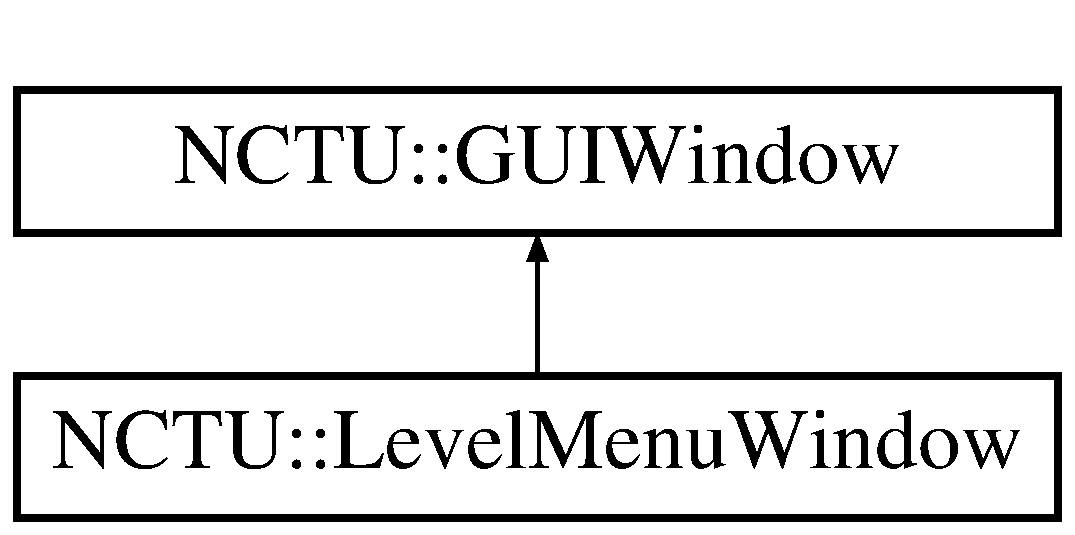
\includegraphics[height=2.000000cm]{class_n_c_t_u_1_1_level_menu_window}
\end{center}
\end{figure}
\subsection*{Public Member Functions}
\begin{DoxyCompactItemize}
\item 
\hyperlink{class_n_c_t_u_1_1_level_menu_window_afeec578e03f2484d2b944e87d75b4390}{Level\+Menu\+Window} ()\hypertarget{class_n_c_t_u_1_1_level_menu_window_afeec578e03f2484d2b944e87d75b4390}{}\label{class_n_c_t_u_1_1_level_menu_window_afeec578e03f2484d2b944e87d75b4390}

\begin{DoxyCompactList}\small\item\em constructor \end{DoxyCompactList}\item 
void \hyperlink{class_n_c_t_u_1_1_level_menu_window_a71a268adcfe5e54548cde85ac721c460}{update\+Disable\+State} ()\hypertarget{class_n_c_t_u_1_1_level_menu_window_a71a268adcfe5e54548cde85ac721c460}{}\label{class_n_c_t_u_1_1_level_menu_window_a71a268adcfe5e54548cde85ac721c460}

\begin{DoxyCompactList}\small\item\em refresh disable state for button \end{DoxyCompactList}\item 
virtual void \hyperlink{class_n_c_t_u_1_1_level_menu_window_aa7ff80563c2fa737d0df71d6ef4ff69d}{set\+Visible} (bool visible)\hypertarget{class_n_c_t_u_1_1_level_menu_window_aa7ff80563c2fa737d0df71d6ef4ff69d}{}\label{class_n_c_t_u_1_1_level_menu_window_aa7ff80563c2fa737d0df71d6ef4ff69d}

\begin{DoxyCompactList}\small\item\em set visibility for this window \end{DoxyCompactList}\end{DoxyCompactItemize}
\subsection*{Protected Member Functions}
\begin{DoxyCompactItemize}
\item 
virtual void \hyperlink{class_n_c_t_u_1_1_level_menu_window_a44e082fb42481f4e35e137feaf496279}{register\+Handlers} ()\hypertarget{class_n_c_t_u_1_1_level_menu_window_a44e082fb42481f4e35e137feaf496279}{}\label{class_n_c_t_u_1_1_level_menu_window_a44e082fb42481f4e35e137feaf496279}

\begin{DoxyCompactList}\small\item\em register event handler \end{DoxyCompactList}\item 
bool \hyperlink{class_n_c_t_u_1_1_level_menu_window_a25b3e0c122775b66a69343e112b9d49c}{on\+Press\+Level1} (const C\+E\+G\+U\+I\+::\+Event\+Args \&e)\hypertarget{class_n_c_t_u_1_1_level_menu_window_a25b3e0c122775b66a69343e112b9d49c}{}\label{class_n_c_t_u_1_1_level_menu_window_a25b3e0c122775b66a69343e112b9d49c}

\begin{DoxyCompactList}\small\item\em process when pressing level 1 \end{DoxyCompactList}\item 
bool \hyperlink{class_n_c_t_u_1_1_level_menu_window_ab238bddb760fed4bb50f92a4e4980923}{on\+Press\+Level2} (const C\+E\+G\+U\+I\+::\+Event\+Args \&e)\hypertarget{class_n_c_t_u_1_1_level_menu_window_ab238bddb760fed4bb50f92a4e4980923}{}\label{class_n_c_t_u_1_1_level_menu_window_ab238bddb760fed4bb50f92a4e4980923}

\begin{DoxyCompactList}\small\item\em process when pressing level 2 \end{DoxyCompactList}\item 
bool \hyperlink{class_n_c_t_u_1_1_level_menu_window_ac9ac75a48ed22a84e5ca5f7e9760a899}{on\+Press\+Level3} (const C\+E\+G\+U\+I\+::\+Event\+Args \&e)\hypertarget{class_n_c_t_u_1_1_level_menu_window_ac9ac75a48ed22a84e5ca5f7e9760a899}{}\label{class_n_c_t_u_1_1_level_menu_window_ac9ac75a48ed22a84e5ca5f7e9760a899}

\begin{DoxyCompactList}\small\item\em process when pressing level 3 \end{DoxyCompactList}\item 
bool \hyperlink{class_n_c_t_u_1_1_level_menu_window_a0ea6a4eb90ebdd516665e56c21065c2f}{on\+Press\+Cancel} (const C\+E\+G\+U\+I\+::\+Event\+Args \&e)\hypertarget{class_n_c_t_u_1_1_level_menu_window_a0ea6a4eb90ebdd516665e56c21065c2f}{}\label{class_n_c_t_u_1_1_level_menu_window_a0ea6a4eb90ebdd516665e56c21065c2f}

\begin{DoxyCompactList}\small\item\em process when pressing cancel button \end{DoxyCompactList}\end{DoxyCompactItemize}
\subsection*{Additional Inherited Members}


\subsection{Detailed Description}
G\+UI window for selecting level. 

The documentation for this class was generated from the following files\+:\begin{DoxyCompactItemize}
\item 
programs/\+Obstacle/include/Level\+Menu\+Window.\+h\item 
programs/\+Obstacle/source/Level\+Menu\+Window.\+cpp\end{DoxyCompactItemize}

\hypertarget{class_n_c_t_u_1_1_main_menu_window}{}\section{N\+C\+TU\+:\+:Main\+Menu\+Window Class Reference}
\label{class_n_c_t_u_1_1_main_menu_window}\index{N\+C\+T\+U\+::\+Main\+Menu\+Window@{N\+C\+T\+U\+::\+Main\+Menu\+Window}}


G\+HI window for main menu.  




{\ttfamily \#include $<$Main\+Menu\+Window.\+h$>$}

Inheritance diagram for N\+C\+TU\+:\+:Main\+Menu\+Window\+:\begin{figure}[H]
\begin{center}
\leavevmode
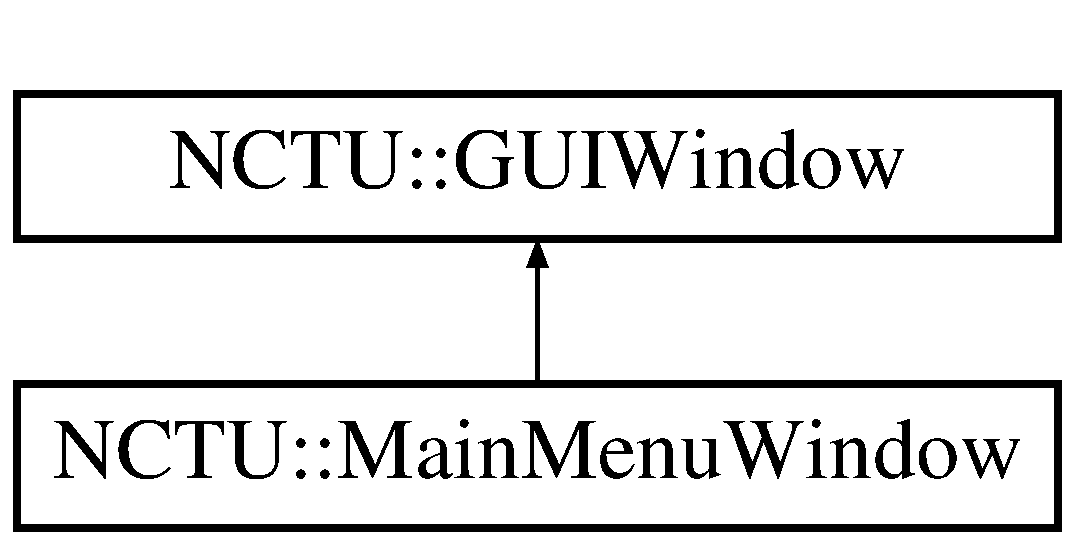
\includegraphics[height=2.000000cm]{class_n_c_t_u_1_1_main_menu_window}
\end{center}
\end{figure}
\subsection*{Public Member Functions}
\begin{DoxyCompactItemize}
\item 
\hyperlink{class_n_c_t_u_1_1_main_menu_window_adefbd912034f753e6e22049f18d947e8}{Main\+Menu\+Window} ()\hypertarget{class_n_c_t_u_1_1_main_menu_window_adefbd912034f753e6e22049f18d947e8}{}\label{class_n_c_t_u_1_1_main_menu_window_adefbd912034f753e6e22049f18d947e8}

\begin{DoxyCompactList}\small\item\em constructor \end{DoxyCompactList}\item 
virtual void \hyperlink{class_n_c_t_u_1_1_main_menu_window_a6587f39dabd84762a2ce44357a372177}{set\+Visible} (bool visible)\hypertarget{class_n_c_t_u_1_1_main_menu_window_a6587f39dabd84762a2ce44357a372177}{}\label{class_n_c_t_u_1_1_main_menu_window_a6587f39dabd84762a2ce44357a372177}

\begin{DoxyCompactList}\small\item\em set visibility for this window \end{DoxyCompactList}\end{DoxyCompactItemize}
\subsection*{Protected Member Functions}
\begin{DoxyCompactItemize}
\item 
virtual void \hyperlink{class_n_c_t_u_1_1_main_menu_window_ac18c70de0ddc81dedaf67f9741631745}{register\+Handlers} ()\hypertarget{class_n_c_t_u_1_1_main_menu_window_ac18c70de0ddc81dedaf67f9741631745}{}\label{class_n_c_t_u_1_1_main_menu_window_ac18c70de0ddc81dedaf67f9741631745}

\begin{DoxyCompactList}\small\item\em register event handler \end{DoxyCompactList}\item 
bool \hyperlink{class_n_c_t_u_1_1_main_menu_window_a41c92268b6622f62daf0838a62c01b48}{on\+Press\+Play} (const C\+E\+G\+U\+I\+::\+Event\+Args \&e)\hypertarget{class_n_c_t_u_1_1_main_menu_window_a41c92268b6622f62daf0838a62c01b48}{}\label{class_n_c_t_u_1_1_main_menu_window_a41c92268b6622f62daf0838a62c01b48}

\begin{DoxyCompactList}\small\item\em process when press play button \end{DoxyCompactList}\item 
bool \hyperlink{class_n_c_t_u_1_1_main_menu_window_a05b6e1700030580fd935263e5758f415}{on\+Press\+Level} (const C\+E\+G\+U\+I\+::\+Event\+Args \&e)\hypertarget{class_n_c_t_u_1_1_main_menu_window_a05b6e1700030580fd935263e5758f415}{}\label{class_n_c_t_u_1_1_main_menu_window_a05b6e1700030580fd935263e5758f415}

\begin{DoxyCompactList}\small\item\em process when press level select button \end{DoxyCompactList}\item 
bool \hyperlink{class_n_c_t_u_1_1_main_menu_window_aca5070bca956bd79efd73dd05e460784}{on\+Press\+Exit} (const C\+E\+G\+U\+I\+::\+Event\+Args \&e)\hypertarget{class_n_c_t_u_1_1_main_menu_window_aca5070bca956bd79efd73dd05e460784}{}\label{class_n_c_t_u_1_1_main_menu_window_aca5070bca956bd79efd73dd05e460784}

\begin{DoxyCompactList}\small\item\em process when press exit button \end{DoxyCompactList}\end{DoxyCompactItemize}
\subsection*{Additional Inherited Members}


\subsection{Detailed Description}
G\+HI window for main menu. 

The documentation for this class was generated from the following files\+:\begin{DoxyCompactItemize}
\item 
programs/\+Obstacle/include/Main\+Menu\+Window.\+h\item 
programs/\+Obstacle/source/Main\+Menu\+Window.\+cpp\end{DoxyCompactItemize}

\hypertarget{class_n_c_t_u_camera}{}\section{N\+C\+T\+U\+Camera Class Reference}
\label{class_n_c_t_u_camera}\index{N\+C\+T\+U\+Camera@{N\+C\+T\+U\+Camera}}


Camera controller for this project.  




{\ttfamily \#include $<$N\+C\+T\+U\+Camera.\+h$>$}

\subsection*{Public Types}
\begin{DoxyCompactItemize}
\item 
enum \hyperlink{class_n_c_t_u_camera_a375160f41c982180edf9a658e316ef58}{Turning\+State} \{ {\bfseries S\+T\+A\+T\+E\+\_\+\+T\+U\+R\+N\+I\+NG}, 
{\bfseries S\+T\+A\+T\+E\+\_\+\+N\+O\+R\+M\+AL}
 \}\hypertarget{class_n_c_t_u_camera_a375160f41c982180edf9a658e316ef58}{}\label{class_n_c_t_u_camera_a375160f41c982180edf9a658e316ef58}
\begin{DoxyCompactList}\small\item\em state declaration of turning / normal \end{DoxyCompactList}
\end{DoxyCompactItemize}
\subsection*{Public Member Functions}
\begin{DoxyCompactItemize}
\item 
\hyperlink{class_n_c_t_u_camera_a38abb4f6c1f26d057b67a5f4dc442f93}{N\+C\+T\+U\+Camera} ()\hypertarget{class_n_c_t_u_camera_a38abb4f6c1f26d057b67a5f4dc442f93}{}\label{class_n_c_t_u_camera_a38abb4f6c1f26d057b67a5f4dc442f93}

\begin{DoxyCompactList}\small\item\em constructor \end{DoxyCompactList}\item 
\hyperlink{class_n_c_t_u_camera_aa90b12d4bb1f0321b734b1e540876d01}{$\sim$\+N\+C\+T\+U\+Camera} (void)\hypertarget{class_n_c_t_u_camera_aa90b12d4bb1f0321b734b1e540876d01}{}\label{class_n_c_t_u_camera_aa90b12d4bb1f0321b734b1e540876d01}

\begin{DoxyCompactList}\small\item\em destructor \end{DoxyCompactList}\item 
void \hyperlink{class_n_c_t_u_camera_a759e64b0b2f3c582733599197d86bcd1}{setup} (Camera $\ast$camera, Scene\+Manager $\ast$Scene\+Mgr, \hyperlink{class_basic_tutorial__00}{Basic\+Tutorial\+\_\+00} $\ast$app)\hypertarget{class_n_c_t_u_camera_a759e64b0b2f3c582733599197d86bcd1}{}\label{class_n_c_t_u_camera_a759e64b0b2f3c582733599197d86bcd1}

\begin{DoxyCompactList}\small\item\em initialize the camera controller with pointers \end{DoxyCompactList}\item 
void \hyperlink{class_n_c_t_u_camera_a94444f8dcbbf4de692d550bfa6ea4a85}{Turn\+Camera} (bool direction, Vector3 Target)\hypertarget{class_n_c_t_u_camera_a94444f8dcbbf4de692d550bfa6ea4a85}{}\label{class_n_c_t_u_camera_a94444f8dcbbf4de692d550bfa6ea4a85}

\begin{DoxyCompactList}\small\item\em turn the camera \end{DoxyCompactList}\item 
void \hyperlink{class_n_c_t_u_camera_ada78a54e693ae248bf210ec5412b1a96}{update\+Basic} (const Frame\+Event \&evt)\hypertarget{class_n_c_t_u_camera_ada78a54e693ae248bf210ec5412b1a96}{}\label{class_n_c_t_u_camera_ada78a54e693ae248bf210ec5412b1a96}

\begin{DoxyCompactList}\small\item\em basic update routine \end{DoxyCompactList}\item 
void \hyperlink{class_n_c_t_u_camera_ae89905594734277ad03ece810a2044f5}{update\+Playing\+Game} (const Frame\+Event \&evt)\hypertarget{class_n_c_t_u_camera_ae89905594734277ad03ece810a2044f5}{}\label{class_n_c_t_u_camera_ae89905594734277ad03ece810a2044f5}

\begin{DoxyCompactList}\small\item\em update routine for playing game \end{DoxyCompactList}\item 
void \hyperlink{class_n_c_t_u_camera_a418e25bc4e93439e0f12fe1074af3fe7}{setup\+Camera} ()\hypertarget{class_n_c_t_u_camera_a418e25bc4e93439e0f12fe1074af3fe7}{}\label{class_n_c_t_u_camera_a418e25bc4e93439e0f12fe1074af3fe7}

\begin{DoxyCompactList}\small\item\em setup controller \end{DoxyCompactList}\item 
bool \hyperlink{class_n_c_t_u_camera_a68c20abf9dd120e315edd033175eef50}{is\+Turn\+OK} () const \hypertarget{class_n_c_t_u_camera_a68c20abf9dd120e315edd033175eef50}{}\label{class_n_c_t_u_camera_a68c20abf9dd120e315edd033175eef50}

\begin{DoxyCompactList}\small\item\em is turning ok for now? \end{DoxyCompactList}\item 
\hyperlink{class_camera_motion}{Camera\+Motion} \& \hyperlink{class_n_c_t_u_camera_a5925e054a060e69c5e252f1bbb63f5e5}{get\+Motion} ()\hypertarget{class_n_c_t_u_camera_a5925e054a060e69c5e252f1bbb63f5e5}{}\label{class_n_c_t_u_camera_a5925e054a060e69c5e252f1bbb63f5e5}

\begin{DoxyCompactList}\small\item\em get the camera motion instance \end{DoxyCompactList}\end{DoxyCompactItemize}
\subsection*{Public Attributes}
\begin{DoxyCompactItemize}
\item 
Vector3 \hyperlink{class_n_c_t_u_camera_ae63ea710bee3e1121ccb7db8b5f1c85f}{m\+Camera\+Position\+Offset}\hypertarget{class_n_c_t_u_camera_ae63ea710bee3e1121ccb7db8b5f1c85f}{}\label{class_n_c_t_u_camera_ae63ea710bee3e1121ccb7db8b5f1c85f}

\begin{DoxyCompactList}\small\item\em camera position offset \end{DoxyCompactList}\item 
Vector3 \hyperlink{class_n_c_t_u_camera_ae1343563fb5952a7bf7394f70858059e}{m\+Camera\+Look\+At\+Offset}\hypertarget{class_n_c_t_u_camera_ae1343563fb5952a7bf7394f70858059e}{}\label{class_n_c_t_u_camera_ae1343563fb5952a7bf7394f70858059e}

\begin{DoxyCompactList}\small\item\em camera look\+At offset \end{DoxyCompactList}\item 
Vector3 \hyperlink{class_n_c_t_u_camera_a414b533b2b30e3f73f950b93e7fe8f1b}{m\+Camera\+Init\+Look\+At}\hypertarget{class_n_c_t_u_camera_a414b533b2b30e3f73f950b93e7fe8f1b}{}\label{class_n_c_t_u_camera_a414b533b2b30e3f73f950b93e7fe8f1b}

\begin{DoxyCompactList}\small\item\em camera initial look\+At \end{DoxyCompactList}\item 
Vector3 \hyperlink{class_n_c_t_u_camera_af0f6d56adf8eef2d1b5494e0e59acbf2}{m\+Camera\+Init\+Position}\hypertarget{class_n_c_t_u_camera_af0f6d56adf8eef2d1b5494e0e59acbf2}{}\label{class_n_c_t_u_camera_af0f6d56adf8eef2d1b5494e0e59acbf2}

\begin{DoxyCompactList}\small\item\em camera initial position \end{DoxyCompactList}\item 
Quaternion \hyperlink{class_n_c_t_u_camera_aba9100e74f7f1349069e091b19b96283}{m\+Init\+Orientation}\hypertarget{class_n_c_t_u_camera_aba9100e74f7f1349069e091b19b96283}{}\label{class_n_c_t_u_camera_aba9100e74f7f1349069e091b19b96283}

\begin{DoxyCompactList}\small\item\em camera initial orientation \end{DoxyCompactList}\item 
int \hyperlink{class_n_c_t_u_camera_af97c1ee5da887f581940ad33c9d42dc5}{m\+Near\+Clip\+Min}\hypertarget{class_n_c_t_u_camera_af97c1ee5da887f581940ad33c9d42dc5}{}\label{class_n_c_t_u_camera_af97c1ee5da887f581940ad33c9d42dc5}

\begin{DoxyCompactList}\small\item\em minimum near clip distance \end{DoxyCompactList}\item 
int \hyperlink{class_n_c_t_u_camera_ac2144233de8a94f1aee27567750f0b7a}{m\+Near\+Clip\+Max}\hypertarget{class_n_c_t_u_camera_ac2144233de8a94f1aee27567750f0b7a}{}\label{class_n_c_t_u_camera_ac2144233de8a94f1aee27567750f0b7a}

\begin{DoxyCompactList}\small\item\em maximum near clip distance \end{DoxyCompactList}\end{DoxyCompactItemize}
\subsection*{Static Public Attributes}
\begin{DoxyCompactItemize}
\item 
static const Real \hyperlink{class_n_c_t_u_camera_a1aba52f772c07e125be557b1e91da5c0}{T\+U\+R\+N\+I\+N\+G\+\_\+\+T\+I\+ME} = 0.\+2/90\hypertarget{class_n_c_t_u_camera_a1aba52f772c07e125be557b1e91da5c0}{}\label{class_n_c_t_u_camera_a1aba52f772c07e125be557b1e91da5c0}

\begin{DoxyCompactList}\small\item\em turning time \end{DoxyCompactList}\end{DoxyCompactItemize}


\subsection{Detailed Description}
Camera controller for this project. 

The documentation for this class was generated from the following files\+:\begin{DoxyCompactItemize}
\item 
programs/\+Obstacle/include/N\+C\+T\+U\+Camera.\+h\item 
programs/\+Obstacle/source/N\+C\+T\+U\+Camera.\+cpp\end{DoxyCompactItemize}

\hypertarget{class_ogre_1_1node_property}{}\section{Ogre\+:\+:node\+Property Class Reference}
\label{class_ogre_1_1node_property}\index{Ogre\+::node\+Property@{Ogre\+::node\+Property}}


store properties for a node  




{\ttfamily \#include $<$Dot\+Scene\+Loader.\+h$>$}

\subsection*{Public Member Functions}
\begin{DoxyCompactItemize}
\item 
\hyperlink{class_ogre_1_1node_property_ae092388b17f66e4171a8ee11e0837e7d}{node\+Property} (const String \&node, const String \&property\+Name, const String \&value, const String \&type)\hypertarget{class_ogre_1_1node_property_ae092388b17f66e4171a8ee11e0837e7d}{}\label{class_ogre_1_1node_property_ae092388b17f66e4171a8ee11e0837e7d}

\begin{DoxyCompactList}\small\item\em constructor \end{DoxyCompactList}\end{DoxyCompactItemize}
\subsection*{Public Attributes}
\begin{DoxyCompactItemize}
\item 
String \hyperlink{class_ogre_1_1node_property_ab384a23c387d1a563ab18e273761e76b}{node\+Name}\hypertarget{class_ogre_1_1node_property_ab384a23c387d1a563ab18e273761e76b}{}\label{class_ogre_1_1node_property_ab384a23c387d1a563ab18e273761e76b}

\begin{DoxyCompactList}\small\item\em name of node \end{DoxyCompactList}\item 
String \hyperlink{class_ogre_1_1node_property_a1f7f77ea3c31717199424086459b2bdd}{property\+Nm}\hypertarget{class_ogre_1_1node_property_a1f7f77ea3c31717199424086459b2bdd}{}\label{class_ogre_1_1node_property_a1f7f77ea3c31717199424086459b2bdd}

\begin{DoxyCompactList}\small\item\em property name \end{DoxyCompactList}\item 
String \hyperlink{class_ogre_1_1node_property_ae5b83b85b5a38575c7ee784c7a8c36e6}{value\+Name}\hypertarget{class_ogre_1_1node_property_ae5b83b85b5a38575c7ee784c7a8c36e6}{}\label{class_ogre_1_1node_property_ae5b83b85b5a38575c7ee784c7a8c36e6}

\begin{DoxyCompactList}\small\item\em value name \end{DoxyCompactList}\item 
String \hyperlink{class_ogre_1_1node_property_a81d48ac5e4506389f5c7a7733717776b}{type\+Name}\hypertarget{class_ogre_1_1node_property_a81d48ac5e4506389f5c7a7733717776b}{}\label{class_ogre_1_1node_property_a81d48ac5e4506389f5c7a7733717776b}

\begin{DoxyCompactList}\small\item\em value name \end{DoxyCompactList}\end{DoxyCompactItemize}


\subsection{Detailed Description}
store properties for a node 

The documentation for this class was generated from the following file\+:\begin{DoxyCompactItemize}
\item 
programs/\+Obstacle/include/Dot\+Scene\+Loader.\+h\end{DoxyCompactItemize}

\hypertarget{class_n_c_t_u_1_1_obstacle}{}\section{N\+C\+TU\+:\+:Obstacle Class Reference}
\label{class_n_c_t_u_1_1_obstacle}\index{N\+C\+T\+U\+::\+Obstacle@{N\+C\+T\+U\+::\+Obstacle}}


base class for all obstacle  




{\ttfamily \#include $<$N\+C\+T\+U\+Obstacle.\+h$>$}

Inheritance diagram for N\+C\+TU\+:\+:Obstacle\+:\begin{figure}[H]
\begin{center}
\leavevmode
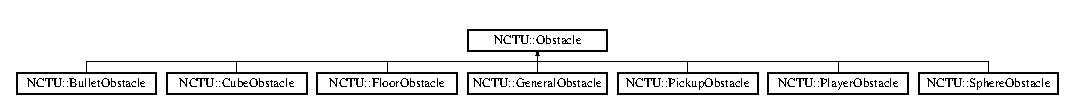
\includegraphics[height=1.038961cm]{class_n_c_t_u_1_1_obstacle}
\end{center}
\end{figure}
\subsection*{Public Member Functions}
\begin{DoxyCompactItemize}
\item 
\hyperlink{class_n_c_t_u_1_1_obstacle_abc03dea67c7426eea315a1ac4da8c78d}{Obstacle} (\hyperlink{class_n_c_t_u_1_1_obstacle_manager}{Obstacle\+Manager} $\ast$mgmt, Ogre\+::\+Real restitution, Ogre\+::\+Real friction, Ogre\+::\+Real mass)\hypertarget{class_n_c_t_u_1_1_obstacle_abc03dea67c7426eea315a1ac4da8c78d}{}\label{class_n_c_t_u_1_1_obstacle_abc03dea67c7426eea315a1ac4da8c78d}

\begin{DoxyCompactList}\small\item\em constructor \end{DoxyCompactList}\item 
\hyperlink{class_n_c_t_u_1_1_obstacle_af96593944da2a5873cdacbd8ff54f076}{Obstacle} (const \hyperlink{class_n_c_t_u_1_1_obstacle}{Obstacle} \&)\hypertarget{class_n_c_t_u_1_1_obstacle_af96593944da2a5873cdacbd8ff54f076}{}\label{class_n_c_t_u_1_1_obstacle_af96593944da2a5873cdacbd8ff54f076}

\begin{DoxyCompactList}\small\item\em copy constructor \end{DoxyCompactList}\item 
virtual \hyperlink{class_n_c_t_u_1_1_obstacle_af2f9cc9c6cff75dca0974fd5ac4f71a9}{$\sim$\+Obstacle} ()\hypertarget{class_n_c_t_u_1_1_obstacle_af2f9cc9c6cff75dca0974fd5ac4f71a9}{}\label{class_n_c_t_u_1_1_obstacle_af2f9cc9c6cff75dca0974fd5ac4f71a9}

\begin{DoxyCompactList}\small\item\em destructor \end{DoxyCompactList}\item 
virtual void \hyperlink{class_n_c_t_u_1_1_obstacle_a12e49360d558e8a875651f212698f3bd}{set\+Scale} (const Ogre\+::\+Vector3 \&)\hypertarget{class_n_c_t_u_1_1_obstacle_a12e49360d558e8a875651f212698f3bd}{}\label{class_n_c_t_u_1_1_obstacle_a12e49360d558e8a875651f212698f3bd}

\begin{DoxyCompactList}\small\item\em set object scale \end{DoxyCompactList}\item 
virtual void \hyperlink{class_n_c_t_u_1_1_obstacle_ad36f7e057a1067bc71dbaf4cef8c7b31}{update\+Collision} (const Ogre\+::\+Frame\+Event \&evt)\hypertarget{class_n_c_t_u_1_1_obstacle_ad36f7e057a1067bc71dbaf4cef8c7b31}{}\label{class_n_c_t_u_1_1_obstacle_ad36f7e057a1067bc71dbaf4cef8c7b31}

\begin{DoxyCompactList}\small\item\em routine for update collision \end{DoxyCompactList}\item 
virtual void \hyperlink{class_n_c_t_u_1_1_obstacle_a45e169430ef20b5ee475f48ca3fc502a}{update\+Life\+Time} (const Ogre\+::\+Frame\+Event \&evt)\hypertarget{class_n_c_t_u_1_1_obstacle_a45e169430ef20b5ee475f48ca3fc502a}{}\label{class_n_c_t_u_1_1_obstacle_a45e169430ef20b5ee475f48ca3fc502a}

\begin{DoxyCompactList}\small\item\em routine for update life time \end{DoxyCompactList}\item 
virtual void \hyperlink{class_n_c_t_u_1_1_obstacle_a232a6f9974ec04ae5ffb1f618f7c6bec}{update\+Playing\+Game} (const Ogre\+::\+Frame\+Event \&evt)\hypertarget{class_n_c_t_u_1_1_obstacle_a232a6f9974ec04ae5ffb1f618f7c6bec}{}\label{class_n_c_t_u_1_1_obstacle_a232a6f9974ec04ae5ffb1f618f7c6bec}

\begin{DoxyCompactList}\small\item\em routine for a playing game \end{DoxyCompactList}\item 
virtual Ogre\+::\+Scene\+Node $\ast$ \hyperlink{class_n_c_t_u_1_1_obstacle_a79f8cc36edef15a3639a40c70acdb53f}{get\+Scene\+Node} ()\hypertarget{class_n_c_t_u_1_1_obstacle_a79f8cc36edef15a3639a40c70acdb53f}{}\label{class_n_c_t_u_1_1_obstacle_a79f8cc36edef15a3639a40c70acdb53f}

\begin{DoxyCompactList}\small\item\em get the scene node \end{DoxyCompactList}\item 
virtual Ogre\+::\+Entity $\ast$ \hyperlink{class_n_c_t_u_1_1_obstacle_ab0b495eb1f91ab76faa751751e3639e7}{get\+Entity} ()\hypertarget{class_n_c_t_u_1_1_obstacle_ab0b495eb1f91ab76faa751751e3639e7}{}\label{class_n_c_t_u_1_1_obstacle_ab0b495eb1f91ab76faa751751e3639e7}

\begin{DoxyCompactList}\small\item\em get the entity \end{DoxyCompactList}\item 
virtual Ogre\+Bullet\+Dynamics\+::\+Rigid\+Body $\ast$ \hyperlink{class_n_c_t_u_1_1_obstacle_aab79cadcfa31f7a6633e4a79df6683ee}{get\+Body} ()\hypertarget{class_n_c_t_u_1_1_obstacle_aab79cadcfa31f7a6633e4a79df6683ee}{}\label{class_n_c_t_u_1_1_obstacle_aab79cadcfa31f7a6633e4a79df6683ee}

\begin{DoxyCompactList}\small\item\em get the bullet rigid body \end{DoxyCompactList}\item 
virtual Ogre\+Bullet\+Collisions\+::\+Collision\+Shape $\ast$ \hyperlink{class_n_c_t_u_1_1_obstacle_aea41027c61d51df4d1ed72c5ad52ae62}{get\+Shape} ()\hypertarget{class_n_c_t_u_1_1_obstacle_aea41027c61d51df4d1ed72c5ad52ae62}{}\label{class_n_c_t_u_1_1_obstacle_aea41027c61d51df4d1ed72c5ad52ae62}

\begin{DoxyCompactList}\small\item\em git the bullet collision shape \end{DoxyCompactList}\item 
virtual void \hyperlink{class_n_c_t_u_1_1_obstacle_a80ef7f5311539939b7ab209c3f42357b}{set\+Velocity} (const Ogre\+::\+Vector3 v)\hypertarget{class_n_c_t_u_1_1_obstacle_a80ef7f5311539939b7ab209c3f42357b}{}\label{class_n_c_t_u_1_1_obstacle_a80ef7f5311539939b7ab209c3f42357b}

\begin{DoxyCompactList}\small\item\em set velocity \end{DoxyCompactList}\item 
virtual Ogre\+::\+Vector3 \hyperlink{class_n_c_t_u_1_1_obstacle_ae3cab20c9bb9dfd905325df76aec46b5}{get\+Velocity} () const \hypertarget{class_n_c_t_u_1_1_obstacle_ae3cab20c9bb9dfd905325df76aec46b5}{}\label{class_n_c_t_u_1_1_obstacle_ae3cab20c9bb9dfd905325df76aec46b5}

\begin{DoxyCompactList}\small\item\em get velocity \end{DoxyCompactList}\item 
virtual void \hyperlink{class_n_c_t_u_1_1_obstacle_a105d2a834de6357bbb159166ed6779ad}{apply\+Velocity\+Change} (const Ogre\+::\+Vector3 v)\hypertarget{class_n_c_t_u_1_1_obstacle_a105d2a834de6357bbb159166ed6779ad}{}\label{class_n_c_t_u_1_1_obstacle_a105d2a834de6357bbb159166ed6779ad}

\begin{DoxyCompactList}\small\item\em apply velocity change \end{DoxyCompactList}\item 
virtual void \hyperlink{class_n_c_t_u_1_1_obstacle_a992c5eabbae44f6c3c2b9cf564bde211}{set\+Position} (const Ogre\+::\+Vector3 v)\hypertarget{class_n_c_t_u_1_1_obstacle_a992c5eabbae44f6c3c2b9cf564bde211}{}\label{class_n_c_t_u_1_1_obstacle_a992c5eabbae44f6c3c2b9cf564bde211}

\begin{DoxyCompactList}\small\item\em set position \end{DoxyCompactList}\item 
virtual Ogre\+::\+Vector3 \hyperlink{class_n_c_t_u_1_1_obstacle_a64c40f6470a9ad47c6441ddef7f8cc62}{get\+Position} () const \hypertarget{class_n_c_t_u_1_1_obstacle_a64c40f6470a9ad47c6441ddef7f8cc62}{}\label{class_n_c_t_u_1_1_obstacle_a64c40f6470a9ad47c6441ddef7f8cc62}

\begin{DoxyCompactList}\small\item\em get position \end{DoxyCompactList}\item 
virtual void \hyperlink{class_n_c_t_u_1_1_obstacle_aa68682ec1330c69bf6093699a42610ff}{set\+Orientation} (const Ogre\+::\+Quaternion q)\hypertarget{class_n_c_t_u_1_1_obstacle_aa68682ec1330c69bf6093699a42610ff}{}\label{class_n_c_t_u_1_1_obstacle_aa68682ec1330c69bf6093699a42610ff}

\begin{DoxyCompactList}\small\item\em set orientation \end{DoxyCompactList}\item 
virtual Ogre\+::\+Quaternion \hyperlink{class_n_c_t_u_1_1_obstacle_aadc30d1638cee2b7eb76fb83cd84cfc2}{get\+Orientation} () const \hypertarget{class_n_c_t_u_1_1_obstacle_aadc30d1638cee2b7eb76fb83cd84cfc2}{}\label{class_n_c_t_u_1_1_obstacle_aadc30d1638cee2b7eb76fb83cd84cfc2}

\begin{DoxyCompactList}\small\item\em get orieatation \end{DoxyCompactList}\item 
virtual void \hyperlink{class_n_c_t_u_1_1_obstacle_aa7271e6282b29e9604e1e36c033c5260}{set\+On\+Floor} (bool val)\hypertarget{class_n_c_t_u_1_1_obstacle_aa7271e6282b29e9604e1e36c033c5260}{}\label{class_n_c_t_u_1_1_obstacle_aa7271e6282b29e9604e1e36c033c5260}

\begin{DoxyCompactList}\small\item\em set the on floor state \end{DoxyCompactList}\item 
virtual bool \hyperlink{class_n_c_t_u_1_1_obstacle_ad286ab7a7891af2fdbe68509414a7091}{get\+On\+Floor} (int threshold=F\+L\+O\+O\+R\+\_\+\+T\+O\+U\+C\+H\+\_\+\+T\+H\+R\+E\+S\+H\+O\+LD) const \hypertarget{class_n_c_t_u_1_1_obstacle_ad286ab7a7891af2fdbe68509414a7091}{}\label{class_n_c_t_u_1_1_obstacle_ad286ab7a7891af2fdbe68509414a7091}

\begin{DoxyCompactList}\small\item\em get the on floor state \end{DoxyCompactList}\item 
virtual bool \hyperlink{class_n_c_t_u_1_1_obstacle_ae419fab10dbf0d0a12fd2648ac4e2d52}{is\+On\+Floor} (int threshold=F\+L\+O\+O\+R\+\_\+\+T\+O\+U\+C\+H\+\_\+\+T\+H\+R\+E\+S\+H\+O\+LD) const \hypertarget{class_n_c_t_u_1_1_obstacle_ae419fab10dbf0d0a12fd2648ac4e2d52}{}\label{class_n_c_t_u_1_1_obstacle_ae419fab10dbf0d0a12fd2648ac4e2d52}

\begin{DoxyCompactList}\small\item\em is on floor? \end{DoxyCompactList}\item 
virtual void \hyperlink{class_n_c_t_u_1_1_obstacle_a72befedacbcc24f006b6e6e06be49cf5}{set\+Is\+Bump\+Obstacle} (bool val)\hypertarget{class_n_c_t_u_1_1_obstacle_a72befedacbcc24f006b6e6e06be49cf5}{}\label{class_n_c_t_u_1_1_obstacle_a72befedacbcc24f006b6e6e06be49cf5}

\begin{DoxyCompactList}\small\item\em set the bump obstacle state \end{DoxyCompactList}\item 
virtual bool \hyperlink{class_n_c_t_u_1_1_obstacle_a6a6cd290bd731357b99d9f94925632fb}{get\+Is\+Bump\+Obstacle} () const \hypertarget{class_n_c_t_u_1_1_obstacle_a6a6cd290bd731357b99d9f94925632fb}{}\label{class_n_c_t_u_1_1_obstacle_a6a6cd290bd731357b99d9f94925632fb}

\begin{DoxyCompactList}\small\item\em get the bump obstacle state \end{DoxyCompactList}\item 
virtual bool \hyperlink{class_n_c_t_u_1_1_obstacle_a22fcf620d1a4592c3cce9dac4f344555}{Is\+Bump\+Obstacle} () const \hypertarget{class_n_c_t_u_1_1_obstacle_a22fcf620d1a4592c3cce9dac4f344555}{}\label{class_n_c_t_u_1_1_obstacle_a22fcf620d1a4592c3cce9dac4f344555}

\begin{DoxyCompactList}\small\item\em is bump obstacle? \end{DoxyCompactList}\item 
virtual void \hyperlink{class_n_c_t_u_1_1_obstacle_a28463f2b0bd1a97128757b58d848bf1f}{on\+Bullet\+Hit} (\hyperlink{class_n_c_t_u_1_1_bullet_obstacle}{Bullet\+Obstacle} $\ast$, \hyperlink{class_n_c_t_u_1_1_obstacle}{Obstacle} $\ast$)\hypertarget{class_n_c_t_u_1_1_obstacle_a28463f2b0bd1a97128757b58d848bf1f}{}\label{class_n_c_t_u_1_1_obstacle_a28463f2b0bd1a97128757b58d848bf1f}

\begin{DoxyCompactList}\small\item\em process on bullet hit \end{DoxyCompactList}\item 
virtual void \hyperlink{class_n_c_t_u_1_1_obstacle_a156ca87f893b7ff453a5180a27564e0b}{set\+Is\+On\+Obstacle\+Plane} (bool val)\hypertarget{class_n_c_t_u_1_1_obstacle_a156ca87f893b7ff453a5180a27564e0b}{}\label{class_n_c_t_u_1_1_obstacle_a156ca87f893b7ff453a5180a27564e0b}

\begin{DoxyCompactList}\small\item\em set on obstacle plane state \end{DoxyCompactList}\item 
virtual bool \hyperlink{class_n_c_t_u_1_1_obstacle_a97c1418cc9898305b231c3cc77aae307}{get\+Is\+On\+Obstacle\+Plane} (int threshold=O\+B\+S\+T\+A\+C\+L\+E\+\_\+\+P\+L\+A\+N\+E\+\_\+\+T\+O\+U\+C\+H\+\_\+\+T\+H\+R\+E\+S\+H\+O\+LD) const \hypertarget{class_n_c_t_u_1_1_obstacle_a97c1418cc9898305b231c3cc77aae307}{}\label{class_n_c_t_u_1_1_obstacle_a97c1418cc9898305b231c3cc77aae307}

\begin{DoxyCompactList}\small\item\em get on obstacle plane state \end{DoxyCompactList}\item 
virtual bool \hyperlink{class_n_c_t_u_1_1_obstacle_a643dc58d043d26db4e1029e5c3c478db}{Is\+On\+Obstacle\+Plane} (int threshold=O\+B\+S\+T\+A\+C\+L\+E\+\_\+\+P\+L\+A\+N\+E\+\_\+\+T\+O\+U\+C\+H\+\_\+\+T\+H\+R\+E\+S\+H\+O\+LD) const \hypertarget{class_n_c_t_u_1_1_obstacle_a643dc58d043d26db4e1029e5c3c478db}{}\label{class_n_c_t_u_1_1_obstacle_a643dc58d043d26db4e1029e5c3c478db}

\begin{DoxyCompactList}\small\item\em is on obstacle plane? \end{DoxyCompactList}\item 
virtual void \hyperlink{class_n_c_t_u_1_1_obstacle_ad081dc72bebac094289d949bf98ee3be}{set\+My\+Iterator} (std\+::list$<$ \hyperlink{class_n_c_t_u_1_1_obstacle}{Obstacle} $\ast$ $>$\+::iterator it)\hypertarget{class_n_c_t_u_1_1_obstacle_ad081dc72bebac094289d949bf98ee3be}{}\label{class_n_c_t_u_1_1_obstacle_ad081dc72bebac094289d949bf98ee3be}

\begin{DoxyCompactList}\small\item\em set my iterator for manager \end{DoxyCompactList}\item 
virtual void \hyperlink{class_n_c_t_u_1_1_obstacle_ac1ec2583dbf455a82c7f4a9566c31f48}{clean\+Up} ()\hypertarget{class_n_c_t_u_1_1_obstacle_ac1ec2583dbf455a82c7f4a9566c31f48}{}\label{class_n_c_t_u_1_1_obstacle_ac1ec2583dbf455a82c7f4a9566c31f48}

\begin{DoxyCompactList}\small\item\em clean up routing \end{DoxyCompactList}\item 
virtual void \hyperlink{class_n_c_t_u_1_1_obstacle_afdce3149f34e8dd84dffe2c954d05e99}{on\+Life\+End} ()\hypertarget{class_n_c_t_u_1_1_obstacle_afdce3149f34e8dd84dffe2c954d05e99}{}\label{class_n_c_t_u_1_1_obstacle_afdce3149f34e8dd84dffe2c954d05e99}

\begin{DoxyCompactList}\small\item\em process on life ended \end{DoxyCompactList}\item 
virtual void \hyperlink{class_n_c_t_u_1_1_obstacle_a06a36fae4b8fcb9ab7939e21e11df1d6}{destroy\+Physics} ()\hypertarget{class_n_c_t_u_1_1_obstacle_a06a36fae4b8fcb9ab7939e21e11df1d6}{}\label{class_n_c_t_u_1_1_obstacle_a06a36fae4b8fcb9ab7939e21e11df1d6}

\begin{DoxyCompactList}\small\item\em destory physics system \end{DoxyCompactList}\item 
virtual void \hyperlink{class_n_c_t_u_1_1_obstacle_ad13df4a17603e10661585509138e8037}{detach\+Entity} ()\hypertarget{class_n_c_t_u_1_1_obstacle_ad13df4a17603e10661585509138e8037}{}\label{class_n_c_t_u_1_1_obstacle_ad13df4a17603e10661585509138e8037}

\begin{DoxyCompactList}\small\item\em detach entity \end{DoxyCompactList}\item 
virtual bool \hyperlink{class_n_c_t_u_1_1_obstacle_af3a33b113a56ba0191b892829d761502}{is\+Alive} () const \hypertarget{class_n_c_t_u_1_1_obstacle_af3a33b113a56ba0191b892829d761502}{}\label{class_n_c_t_u_1_1_obstacle_af3a33b113a56ba0191b892829d761502}

\begin{DoxyCompactList}\small\item\em is alive? \end{DoxyCompactList}\item 
virtual bool \hyperlink{class_n_c_t_u_1_1_obstacle_a7b3760f178b3299589706eb720210087}{need\+Deleted} () const \hypertarget{class_n_c_t_u_1_1_obstacle_a7b3760f178b3299589706eb720210087}{}\label{class_n_c_t_u_1_1_obstacle_a7b3760f178b3299589706eb720210087}

\begin{DoxyCompactList}\small\item\em is need to be deleted? \end{DoxyCompactList}\item 
virtual void \hyperlink{class_n_c_t_u_1_1_obstacle_a1e444ec09571654d3a2d18a68d8bb9eb}{set\+Life\+Time} (Ogre\+::\+Real v)\hypertarget{class_n_c_t_u_1_1_obstacle_a1e444ec09571654d3a2d18a68d8bb9eb}{}\label{class_n_c_t_u_1_1_obstacle_a1e444ec09571654d3a2d18a68d8bb9eb}

\begin{DoxyCompactList}\small\item\em set life time \end{DoxyCompactList}\item 
virtual void \hyperlink{class_n_c_t_u_1_1_obstacle_a4300351847149b550c72826721e3d2aa}{cancel\+Life\+Time} ()\hypertarget{class_n_c_t_u_1_1_obstacle_a4300351847149b550c72826721e3d2aa}{}\label{class_n_c_t_u_1_1_obstacle_a4300351847149b550c72826721e3d2aa}

\begin{DoxyCompactList}\small\item\em cancel life time \end{DoxyCompactList}\item 
virtual void \hyperlink{class_n_c_t_u_1_1_obstacle_a41c126bdbf76855a5ba645a5d74024cb}{set\+Hit\+Point} (int val, Hp\+Type type)\hypertarget{class_n_c_t_u_1_1_obstacle_a41c126bdbf76855a5ba645a5d74024cb}{}\label{class_n_c_t_u_1_1_obstacle_a41c126bdbf76855a5ba645a5d74024cb}

\begin{DoxyCompactList}\small\item\em set the hit point \end{DoxyCompactList}\item 
virtual int \hyperlink{class_n_c_t_u_1_1_obstacle_a3e010ae1903baacc5991a6ff677d70f2}{get\+Hit\+Point} () const \hypertarget{class_n_c_t_u_1_1_obstacle_a3e010ae1903baacc5991a6ff677d70f2}{}\label{class_n_c_t_u_1_1_obstacle_a3e010ae1903baacc5991a6ff677d70f2}

\begin{DoxyCompactList}\small\item\em get the hit point \end{DoxyCompactList}\item 
virtual bool \hyperlink{class_n_c_t_u_1_1_obstacle_a65e0fa8a3b943571a7408e7b6242bea1}{is\+Invincible} () const \hypertarget{class_n_c_t_u_1_1_obstacle_a65e0fa8a3b943571a7408e7b6242bea1}{}\label{class_n_c_t_u_1_1_obstacle_a65e0fa8a3b943571a7408e7b6242bea1}

\begin{DoxyCompactList}\small\item\em is invincible? \end{DoxyCompactList}\item 
virtual void \hyperlink{class_n_c_t_u_1_1_obstacle_a4b7ee4353297cd13f73f7a9e2e851264}{init\+Particle\+System} (const Ogre\+::\+String \&particle\+Name, int index=0)\hypertarget{class_n_c_t_u_1_1_obstacle_a4b7ee4353297cd13f73f7a9e2e851264}{}\label{class_n_c_t_u_1_1_obstacle_a4b7ee4353297cd13f73f7a9e2e851264}

\begin{DoxyCompactList}\small\item\em initialize the particle system \end{DoxyCompactList}\item 
virtual void \hyperlink{class_n_c_t_u_1_1_obstacle_ab6bf4ec6684528fca9b1e4cf7a273cc3}{set\+Off\+Particle\+System} (int index=0)\hypertarget{class_n_c_t_u_1_1_obstacle_ab6bf4ec6684528fca9b1e4cf7a273cc3}{}\label{class_n_c_t_u_1_1_obstacle_ab6bf4ec6684528fca9b1e4cf7a273cc3}

\begin{DoxyCompactList}\small\item\em set off the particle system \end{DoxyCompactList}\item 
virtual void \hyperlink{class_n_c_t_u_1_1_obstacle_aa156cccecda15fcfb0a51bf2fe93be07}{stop\+Particle\+System} (int index=0)\hypertarget{class_n_c_t_u_1_1_obstacle_aa156cccecda15fcfb0a51bf2fe93be07}{}\label{class_n_c_t_u_1_1_obstacle_aa156cccecda15fcfb0a51bf2fe93be07}

\begin{DoxyCompactList}\small\item\em stop the particle system \end{DoxyCompactList}\item 
virtual void \hyperlink{class_n_c_t_u_1_1_obstacle_a616b49cf5897581a78308498b3fbd15a}{destroy\+Particle\+System} ()\hypertarget{class_n_c_t_u_1_1_obstacle_a616b49cf5897581a78308498b3fbd15a}{}\label{class_n_c_t_u_1_1_obstacle_a616b49cf5897581a78308498b3fbd15a}

\begin{DoxyCompactList}\small\item\em destroy the particle system \end{DoxyCompactList}\item 
virtual Hp\+Type \hyperlink{class_n_c_t_u_1_1_obstacle_a6314a48b3bf0b389f2718bca6a6ba226}{get\+Hp\+Type} () const \hypertarget{class_n_c_t_u_1_1_obstacle_a6314a48b3bf0b389f2718bca6a6ba226}{}\label{class_n_c_t_u_1_1_obstacle_a6314a48b3bf0b389f2718bca6a6ba226}

\begin{DoxyCompactList}\small\item\em get hp type \end{DoxyCompactList}\item 
virtual int \hyperlink{class_n_c_t_u_1_1_obstacle_aaec0ed1185982b1d2507a8d24adcfdfc}{decrease\+Hp} (int value=1)\hypertarget{class_n_c_t_u_1_1_obstacle_aaec0ed1185982b1d2507a8d24adcfdfc}{}\label{class_n_c_t_u_1_1_obstacle_aaec0ed1185982b1d2507a8d24adcfdfc}

\begin{DoxyCompactList}\small\item\em decrease hp \end{DoxyCompactList}\item 
virtual void \hyperlink{class_n_c_t_u_1_1_obstacle_ad89e5a33bf7f5aa52a46370cd7162a4b}{set\+Bump\+Speed} (Ogre\+::\+Real val)\hypertarget{class_n_c_t_u_1_1_obstacle_ad89e5a33bf7f5aa52a46370cd7162a4b}{}\label{class_n_c_t_u_1_1_obstacle_ad89e5a33bf7f5aa52a46370cd7162a4b}

\begin{DoxyCompactList}\small\item\em set bump-\/jump speed \end{DoxyCompactList}\item 
virtual Ogre\+::\+Real \hyperlink{class_n_c_t_u_1_1_obstacle_a342a664e19976891d45d9309821f1d81}{get\+Bump\+Speed} () const \hypertarget{class_n_c_t_u_1_1_obstacle_a342a664e19976891d45d9309821f1d81}{}\label{class_n_c_t_u_1_1_obstacle_a342a664e19976891d45d9309821f1d81}

\begin{DoxyCompactList}\small\item\em get bump-\/jump speed \end{DoxyCompactList}\item 
virtual \hyperlink{class_n_c_t_u_1_1_obstacle_manager}{Obstacle\+Manager} $\ast$ \hyperlink{class_n_c_t_u_1_1_obstacle_a2c909e22367353721b9efad22cffd190}{get\+Manager} ()\hypertarget{class_n_c_t_u_1_1_obstacle_a2c909e22367353721b9efad22cffd190}{}\label{class_n_c_t_u_1_1_obstacle_a2c909e22367353721b9efad22cffd190}

\begin{DoxyCompactList}\small\item\em get the obstacle manager \end{DoxyCompactList}\item 
virtual void \hyperlink{class_n_c_t_u_1_1_obstacle_aa1aec7492db31b24b428290ad34e5058}{set\+Current\+Obstacle} (\hyperlink{class_n_c_t_u_1_1_obstacle}{Obstacle} $\ast$obj)\hypertarget{class_n_c_t_u_1_1_obstacle_aa1aec7492db31b24b428290ad34e5058}{}\label{class_n_c_t_u_1_1_obstacle_aa1aec7492db31b24b428290ad34e5058}

\begin{DoxyCompactList}\small\item\em set current obstacle touched \end{DoxyCompactList}\item 
virtual void \hyperlink{class_n_c_t_u_1_1_obstacle_aa062441e739d95d31f5f8489229d86ca}{set\+Turn\+Type} (const Ogre\+::\+String \&v)\hypertarget{class_n_c_t_u_1_1_obstacle_aa062441e739d95d31f5f8489229d86ca}{}\label{class_n_c_t_u_1_1_obstacle_aa062441e739d95d31f5f8489229d86ca}

\begin{DoxyCompactList}\small\item\em set turn type \end{DoxyCompactList}\item 
virtual const Ogre\+::\+String \& \hyperlink{class_n_c_t_u_1_1_obstacle_ad67378fa3bac4797e8028388021859aa}{get\+Turn\+Type} () const \hypertarget{class_n_c_t_u_1_1_obstacle_ad67378fa3bac4797e8028388021859aa}{}\label{class_n_c_t_u_1_1_obstacle_ad67378fa3bac4797e8028388021859aa}

\begin{DoxyCompactList}\small\item\em get turn type \end{DoxyCompactList}\item 
virtual void \hyperlink{class_n_c_t_u_1_1_obstacle_a5024c55cbbe88f55e811f6d8f79f63c1}{set\+Turn\+Used} (bool v)\hypertarget{class_n_c_t_u_1_1_obstacle_a5024c55cbbe88f55e811f6d8f79f63c1}{}\label{class_n_c_t_u_1_1_obstacle_a5024c55cbbe88f55e811f6d8f79f63c1}

\begin{DoxyCompactList}\small\item\em set turn used state \end{DoxyCompactList}\item 
virtual bool \hyperlink{class_n_c_t_u_1_1_obstacle_a529732a75d861258223e9389e555d138}{get\+Turn\+Used} () const \hypertarget{class_n_c_t_u_1_1_obstacle_a529732a75d861258223e9389e555d138}{}\label{class_n_c_t_u_1_1_obstacle_a529732a75d861258223e9389e555d138}

\begin{DoxyCompactList}\small\item\em get turn used state \end{DoxyCompactList}\item 
virtual const Ogre\+::\+String \& \hyperlink{class_n_c_t_u_1_1_obstacle_a08a8a4b08b58a763328511e38a5ee507}{get\+Name} () const \hypertarget{class_n_c_t_u_1_1_obstacle_a08a8a4b08b58a763328511e38a5ee507}{}\label{class_n_c_t_u_1_1_obstacle_a08a8a4b08b58a763328511e38a5ee507}

\begin{DoxyCompactList}\small\item\em get name \end{DoxyCompactList}\item 
virtual bool \hyperlink{class_n_c_t_u_1_1_obstacle_aaf76ae2db2319c5d23497e5d1b9250d1}{can\+Be\+Shoot} () const \hypertarget{class_n_c_t_u_1_1_obstacle_aaf76ae2db2319c5d23497e5d1b9250d1}{}\label{class_n_c_t_u_1_1_obstacle_aaf76ae2db2319c5d23497e5d1b9250d1}

\begin{DoxyCompactList}\small\item\em is this object can be shoot? \end{DoxyCompactList}\item 
virtual bool \hyperlink{class_n_c_t_u_1_1_obstacle_abacf17c33a0935723a239614a7c6dccb}{can\+Stand\+On} () const \hypertarget{class_n_c_t_u_1_1_obstacle_abacf17c33a0935723a239614a7c6dccb}{}\label{class_n_c_t_u_1_1_obstacle_abacf17c33a0935723a239614a7c6dccb}

\begin{DoxyCompactList}\small\item\em is this object can be standed on? \end{DoxyCompactList}\item 
virtual bool \hyperlink{class_n_c_t_u_1_1_obstacle_ae43c3acf29c136a4a8a281c55bad529f}{can\+Cause\+Dead} () const \hypertarget{class_n_c_t_u_1_1_obstacle_ae43c3acf29c136a4a8a281c55bad529f}{}\label{class_n_c_t_u_1_1_obstacle_ae43c3acf29c136a4a8a281c55bad529f}

\begin{DoxyCompactList}\small\item\em is this object can cause dead? \end{DoxyCompactList}\item 
virtual void \hyperlink{class_n_c_t_u_1_1_obstacle_a9fd48eeac098f18cb455aeeeb7b48585}{destroy} ()\hypertarget{class_n_c_t_u_1_1_obstacle_a9fd48eeac098f18cb455aeeeb7b48585}{}\label{class_n_c_t_u_1_1_obstacle_a9fd48eeac098f18cb455aeeeb7b48585}

\begin{DoxyCompactList}\small\item\em destory obstacle \end{DoxyCompactList}\item 
virtual void \hyperlink{class_n_c_t_u_1_1_obstacle_a8fc1473e1914a79835f3219488fb4262}{freeze} ()\hypertarget{class_n_c_t_u_1_1_obstacle_a8fc1473e1914a79835f3219488fb4262}{}\label{class_n_c_t_u_1_1_obstacle_a8fc1473e1914a79835f3219488fb4262}

\begin{DoxyCompactList}\small\item\em freeze the obstacle \end{DoxyCompactList}\item 
virtual void \hyperlink{class_n_c_t_u_1_1_obstacle_a597c2eaada64e687454fd6dad0f67c01}{unfreeze} ()\hypertarget{class_n_c_t_u_1_1_obstacle_a597c2eaada64e687454fd6dad0f67c01}{}\label{class_n_c_t_u_1_1_obstacle_a597c2eaada64e687454fd6dad0f67c01}

\begin{DoxyCompactList}\small\item\em unfreeze the obstacle \end{DoxyCompactList}\end{DoxyCompactItemize}
\subsection*{Public Attributes}
\begin{DoxyCompactItemize}
\item 
std\+::deque$<$ std\+::pair$<$ Ogre\+::\+Vector3, Ogre\+::\+Real $>$ $>$ \hyperlink{class_n_c_t_u_1_1_obstacle_a48ed0cbb52a09d2015a6c30edf4942b5}{m\+Collision\+Condition\+Vectors}\hypertarget{class_n_c_t_u_1_1_obstacle_a48ed0cbb52a09d2015a6c30edf4942b5}{}\label{class_n_c_t_u_1_1_obstacle_a48ed0cbb52a09d2015a6c30edf4942b5}

\begin{DoxyCompactList}\small\item\em array of collision condition vectors \end{DoxyCompactList}\item 
\hyperlink{classprop_map}{prop\+Map}$<$ int, Ogre\+::\+String $>$ \hyperlink{class_n_c_t_u_1_1_obstacle_a6d2779250da24bd2b988af7d0ff5f774}{m\+Hp\+Change\+Materials}\hypertarget{class_n_c_t_u_1_1_obstacle_a6d2779250da24bd2b988af7d0ff5f774}{}\label{class_n_c_t_u_1_1_obstacle_a6d2779250da24bd2b988af7d0ff5f774}

\begin{DoxyCompactList}\small\item\em material name for hp change \end{DoxyCompactList}\end{DoxyCompactItemize}
\subsection*{Protected Member Functions}
\begin{DoxyCompactItemize}
\item 
virtual Ogre\+Bullet\+Collisions\+::\+Collision\+Shape $\ast$ \hyperlink{class_n_c_t_u_1_1_obstacle_a226dbf997ccf224cafdb612c3821e944}{generate\+Fitting\+Shape} (Ogre\+::\+Scene\+Node $\ast$node, Ogre\+::\+Entity $\ast$ent)\hypertarget{class_n_c_t_u_1_1_obstacle_a226dbf997ccf224cafdb612c3821e944}{}\label{class_n_c_t_u_1_1_obstacle_a226dbf997ccf224cafdb612c3821e944}

\begin{DoxyCompactList}\small\item\em generate fitting bullet collision shape \end{DoxyCompactList}\item 
virtual Ogre\+Bullet\+Collisions\+::\+Collision\+Shape $\ast$ \hyperlink{class_n_c_t_u_1_1_obstacle_a25a4697df6bd0fe7c45542f443d44578}{generate\+Convex\+Shape} (Ogre\+::\+Scene\+Node $\ast$node, Ogre\+::\+Entity $\ast$ent)\hypertarget{class_n_c_t_u_1_1_obstacle_a25a4697df6bd0fe7c45542f443d44578}{}\label{class_n_c_t_u_1_1_obstacle_a25a4697df6bd0fe7c45542f443d44578}

\begin{DoxyCompactList}\small\item\em generate convex bullet collision shape \end{DoxyCompactList}\end{DoxyCompactItemize}
\subsection*{Protected Attributes}
\begin{DoxyCompactItemize}
\item 
bool \hyperlink{class_n_c_t_u_1_1_obstacle_a4305d4e1560537dc2d83de619976deb3}{m\+Is\+Bump\+Obstacle}\hypertarget{class_n_c_t_u_1_1_obstacle_a4305d4e1560537dc2d83de619976deb3}{}\label{class_n_c_t_u_1_1_obstacle_a4305d4e1560537dc2d83de619976deb3}

\begin{DoxyCompactList}\small\item\em is bump into obstacle? \end{DoxyCompactList}\item 
\hyperlink{class_n_c_t_u_1_1_obstacle_manager}{Obstacle\+Manager} $\ast$ \hyperlink{class_n_c_t_u_1_1_obstacle_ac6f0b6d7230560172417c3bfe1b78582}{m\+Manager}\hypertarget{class_n_c_t_u_1_1_obstacle_ac6f0b6d7230560172417c3bfe1b78582}{}\label{class_n_c_t_u_1_1_obstacle_ac6f0b6d7230560172417c3bfe1b78582}

\begin{DoxyCompactList}\small\item\em pointer to the manager \end{DoxyCompactList}\item 
Ogre\+Bullet\+Dynamics\+::\+Rigid\+Body $\ast$ \hyperlink{class_n_c_t_u_1_1_obstacle_afaa1b0da65edd91625b3eef7d374f4b6}{m\+Body}\hypertarget{class_n_c_t_u_1_1_obstacle_afaa1b0da65edd91625b3eef7d374f4b6}{}\label{class_n_c_t_u_1_1_obstacle_afaa1b0da65edd91625b3eef7d374f4b6}

\begin{DoxyCompactList}\small\item\em pointer to the rigid body \end{DoxyCompactList}\item 
Ogre\+Bullet\+Collisions\+::\+Collision\+Shape $\ast$ \hyperlink{class_n_c_t_u_1_1_obstacle_a4f7c737bb2030cad087cd9c287598d17}{m\+Shape}\hypertarget{class_n_c_t_u_1_1_obstacle_a4f7c737bb2030cad087cd9c287598d17}{}\label{class_n_c_t_u_1_1_obstacle_a4f7c737bb2030cad087cd9c287598d17}

\begin{DoxyCompactList}\small\item\em pointer to the collision shape \end{DoxyCompactList}\item 
Ogre\+::\+Real \hyperlink{class_n_c_t_u_1_1_obstacle_a41e92d725f5cfe94dcd2d45873368d9a}{m\+Restitution}\hypertarget{class_n_c_t_u_1_1_obstacle_a41e92d725f5cfe94dcd2d45873368d9a}{}\label{class_n_c_t_u_1_1_obstacle_a41e92d725f5cfe94dcd2d45873368d9a}

\begin{DoxyCompactList}\small\item\em physics restitution \end{DoxyCompactList}\item 
Ogre\+::\+Real \hyperlink{class_n_c_t_u_1_1_obstacle_a003de6ce7863352fe7e091b231e6a16b}{m\+Friction}\hypertarget{class_n_c_t_u_1_1_obstacle_a003de6ce7863352fe7e091b231e6a16b}{}\label{class_n_c_t_u_1_1_obstacle_a003de6ce7863352fe7e091b231e6a16b}

\begin{DoxyCompactList}\small\item\em physics friction \end{DoxyCompactList}\item 
Ogre\+::\+Real \hyperlink{class_n_c_t_u_1_1_obstacle_a94c0ab710fef9c9c818cb69fbd6d39f6}{m\+Mass}\hypertarget{class_n_c_t_u_1_1_obstacle_a94c0ab710fef9c9c818cb69fbd6d39f6}{}\label{class_n_c_t_u_1_1_obstacle_a94c0ab710fef9c9c818cb69fbd6d39f6}

\begin{DoxyCompactList}\small\item\em physics mass \end{DoxyCompactList}\item 
Ogre\+::\+Scene\+Node $\ast$ \hyperlink{class_n_c_t_u_1_1_obstacle_a964a09c8f078f9338b54a795a730d240}{m\+Node}\hypertarget{class_n_c_t_u_1_1_obstacle_a964a09c8f078f9338b54a795a730d240}{}\label{class_n_c_t_u_1_1_obstacle_a964a09c8f078f9338b54a795a730d240}

\begin{DoxyCompactList}\small\item\em pointer to scene node \end{DoxyCompactList}\item 
Ogre\+::\+Entity $\ast$ \hyperlink{class_n_c_t_u_1_1_obstacle_a44efdd73b8a2b99ad4fd8ed7a097216e}{m\+Entity}\hypertarget{class_n_c_t_u_1_1_obstacle_a44efdd73b8a2b99ad4fd8ed7a097216e}{}\label{class_n_c_t_u_1_1_obstacle_a44efdd73b8a2b99ad4fd8ed7a097216e}

\begin{DoxyCompactList}\small\item\em pointer to entity \end{DoxyCompactList}\item 
Ogre\+::\+String \hyperlink{class_n_c_t_u_1_1_obstacle_a4d2ff7d20cc39546305abb5e2494ecd8}{m\+Name}\hypertarget{class_n_c_t_u_1_1_obstacle_a4d2ff7d20cc39546305abb5e2494ecd8}{}\label{class_n_c_t_u_1_1_obstacle_a4d2ff7d20cc39546305abb5e2494ecd8}

\begin{DoxyCompactList}\small\item\em obstalce name \end{DoxyCompactList}\item 
Ogre\+::\+Vector3 \hyperlink{class_n_c_t_u_1_1_obstacle_a10ede4821f9d584365c60989b692bdce}{m\+Scale\+Difference}\hypertarget{class_n_c_t_u_1_1_obstacle_a10ede4821f9d584365c60989b692bdce}{}\label{class_n_c_t_u_1_1_obstacle_a10ede4821f9d584365c60989b692bdce}

\begin{DoxyCompactList}\small\item\em scale difference of object \end{DoxyCompactList}\item 
int \hyperlink{class_n_c_t_u_1_1_obstacle_ae4321fbbf5bd3b2ece94b588fc043f27}{m\+Floor\+Touch\+Value}\hypertarget{class_n_c_t_u_1_1_obstacle_ae4321fbbf5bd3b2ece94b588fc043f27}{}\label{class_n_c_t_u_1_1_obstacle_ae4321fbbf5bd3b2ece94b588fc043f27}

\begin{DoxyCompactList}\small\item\em floor touch value \end{DoxyCompactList}\item 
int \hyperlink{class_n_c_t_u_1_1_obstacle_afe9bad1107d74ceeb5d6c83ff6635dd5}{m\+Obstacle\+Plane\+Touch\+Value}\hypertarget{class_n_c_t_u_1_1_obstacle_afe9bad1107d74ceeb5d6c83ff6635dd5}{}\label{class_n_c_t_u_1_1_obstacle_afe9bad1107d74ceeb5d6c83ff6635dd5}

\begin{DoxyCompactList}\small\item\em obstacle touch value \end{DoxyCompactList}\item 
Ogre\+::\+Real \hyperlink{class_n_c_t_u_1_1_obstacle_a2cb0c579e7e9e40dd267ff58d42d0fcb}{m\+Life\+Time}\hypertarget{class_n_c_t_u_1_1_obstacle_a2cb0c579e7e9e40dd267ff58d42d0fcb}{}\label{class_n_c_t_u_1_1_obstacle_a2cb0c579e7e9e40dd267ff58d42d0fcb}

\begin{DoxyCompactList}\small\item\em life time \end{DoxyCompactList}\item 
bool \hyperlink{class_n_c_t_u_1_1_obstacle_a2bbefafdf48468b1b8254d884945787d}{m\+Life\+Time\+Enable}\hypertarget{class_n_c_t_u_1_1_obstacle_a2bbefafdf48468b1b8254d884945787d}{}\label{class_n_c_t_u_1_1_obstacle_a2bbefafdf48468b1b8254d884945787d}

\begin{DoxyCompactList}\small\item\em is life time enabled? \end{DoxyCompactList}\item 
bool \hyperlink{class_n_c_t_u_1_1_obstacle_aa407bf6d5805696a4a80f228ca414066}{m\+Delete\+Mark}\hypertarget{class_n_c_t_u_1_1_obstacle_aa407bf6d5805696a4a80f228ca414066}{}\label{class_n_c_t_u_1_1_obstacle_aa407bf6d5805696a4a80f228ca414066}

\begin{DoxyCompactList}\small\item\em is need deleted? \end{DoxyCompactList}\item 
bool \hyperlink{class_n_c_t_u_1_1_obstacle_aeda6730f371a397c5d08dbd733a4123c}{m\+Entity\+Detached}\hypertarget{class_n_c_t_u_1_1_obstacle_aeda6730f371a397c5d08dbd733a4123c}{}\label{class_n_c_t_u_1_1_obstacle_aeda6730f371a397c5d08dbd733a4123c}

\begin{DoxyCompactList}\small\item\em is entity detached? \end{DoxyCompactList}\item 
int \hyperlink{class_n_c_t_u_1_1_obstacle_a8e12006c1230c1147b7a0d49a13db9e1}{m\+Hit\+Point}\hypertarget{class_n_c_t_u_1_1_obstacle_a8e12006c1230c1147b7a0d49a13db9e1}{}\label{class_n_c_t_u_1_1_obstacle_a8e12006c1230c1147b7a0d49a13db9e1}

\begin{DoxyCompactList}\small\item\em hit point \end{DoxyCompactList}\item 
Hp\+Type \hyperlink{class_n_c_t_u_1_1_obstacle_a597fb63280339f18532f87256bb0a3fc}{m\+Hp\+Type}\hypertarget{class_n_c_t_u_1_1_obstacle_a597fb63280339f18532f87256bb0a3fc}{}\label{class_n_c_t_u_1_1_obstacle_a597fb63280339f18532f87256bb0a3fc}

\begin{DoxyCompactList}\small\item\em hp type \end{DoxyCompactList}\item 
Ogre\+::\+Real \hyperlink{class_n_c_t_u_1_1_obstacle_abff327c8d53bfa8c90fe3d1c6a3973b2}{m\+Bump\+Speed}\hypertarget{class_n_c_t_u_1_1_obstacle_abff327c8d53bfa8c90fe3d1c6a3973b2}{}\label{class_n_c_t_u_1_1_obstacle_abff327c8d53bfa8c90fe3d1c6a3973b2}

\begin{DoxyCompactList}\small\item\em bump-\/jump speed \end{DoxyCompactList}\item 
Ogre\+::\+String \hyperlink{class_n_c_t_u_1_1_obstacle_a2bf103c410891ac74c39ef8900f936d6}{m\+Turn\+Type}\hypertarget{class_n_c_t_u_1_1_obstacle_a2bf103c410891ac74c39ef8900f936d6}{}\label{class_n_c_t_u_1_1_obstacle_a2bf103c410891ac74c39ef8900f936d6}

\begin{DoxyCompactList}\small\item\em turn type \end{DoxyCompactList}\item 
bool \hyperlink{class_n_c_t_u_1_1_obstacle_a00ba3567bc37de10576bcb0e4aa0180b}{m\+Turn\+Used}\hypertarget{class_n_c_t_u_1_1_obstacle_a00ba3567bc37de10576bcb0e4aa0180b}{}\label{class_n_c_t_u_1_1_obstacle_a00ba3567bc37de10576bcb0e4aa0180b}

\begin{DoxyCompactList}\small\item\em is turn used? \end{DoxyCompactList}\item 
bool \hyperlink{class_n_c_t_u_1_1_obstacle_a42c01e3c5cf2ac4b96fb78565022e2a9}{m\+Frozen}\hypertarget{class_n_c_t_u_1_1_obstacle_a42c01e3c5cf2ac4b96fb78565022e2a9}{}\label{class_n_c_t_u_1_1_obstacle_a42c01e3c5cf2ac4b96fb78565022e2a9}

\begin{DoxyCompactList}\small\item\em is frozen? \end{DoxyCompactList}\item 
std\+::list$<$ \hyperlink{class_n_c_t_u_1_1_obstacle}{Obstacle} $\ast$ $>$\+::iterator \hyperlink{class_n_c_t_u_1_1_obstacle_a66f871667db677d933413d2a986cc0cc}{m\+My\+Iterator}\hypertarget{class_n_c_t_u_1_1_obstacle_a66f871667db677d933413d2a986cc0cc}{}\label{class_n_c_t_u_1_1_obstacle_a66f871667db677d933413d2a986cc0cc}

\begin{DoxyCompactList}\small\item\em iterator for manager \end{DoxyCompactList}\item 
\hyperlink{class_n_c_t_u_1_1_obstacle}{Obstacle} $\ast$ \hyperlink{class_n_c_t_u_1_1_obstacle_ab0ef4a664fa4320d99e3256f1f50e434}{m\+Current\+Obstacle}\hypertarget{class_n_c_t_u_1_1_obstacle_ab0ef4a664fa4320d99e3256f1f50e434}{}\label{class_n_c_t_u_1_1_obstacle_ab0ef4a664fa4320d99e3256f1f50e434}

\begin{DoxyCompactList}\small\item\em pointer to the current obstacle \end{DoxyCompactList}\item 
Ogre\+::\+Real \hyperlink{class_n_c_t_u_1_1_obstacle_aab0815b13db0dc1cb589ee143f849303}{m\+Current\+Obstacle\+Valid}\hypertarget{class_n_c_t_u_1_1_obstacle_aab0815b13db0dc1cb589ee143f849303}{}\label{class_n_c_t_u_1_1_obstacle_aab0815b13db0dc1cb589ee143f849303}

\begin{DoxyCompactList}\small\item\em valid time for current obstacle \end{DoxyCompactList}\item 
std\+::deque$<$ \hyperlink{struct_n_c_t_u_1_1_particle_system_pack}{Particle\+System\+Pack} $>$ \hyperlink{class_n_c_t_u_1_1_obstacle_a30591db733c980f295b78c1f7f687cfb}{m\+Particle\+Systems}\hypertarget{class_n_c_t_u_1_1_obstacle_a30591db733c980f295b78c1f7f687cfb}{}\label{class_n_c_t_u_1_1_obstacle_a30591db733c980f295b78c1f7f687cfb}

\begin{DoxyCompactList}\small\item\em array of particle system \end{DoxyCompactList}\end{DoxyCompactItemize}


\subsection{Detailed Description}
base class for all obstacle 

The documentation for this class was generated from the following files\+:\begin{DoxyCompactItemize}
\item 
N\+C\+T\+U\+Obstacle/include/N\+C\+T\+U\+Obstacle.\+h\item 
N\+C\+T\+U\+Obstacle/src/N\+C\+T\+U\+Obstacle.\+cpp\end{DoxyCompactItemize}

\hypertarget{struct_n_c_t_u_1_1_obstacle_contact_result_callback}{}\section{N\+C\+TU\+:\+:Obstacle\+Contact\+Result\+Callback Struct Reference}
\label{struct_n_c_t_u_1_1_obstacle_contact_result_callback}\index{N\+C\+T\+U\+::\+Obstacle\+Contact\+Result\+Callback@{N\+C\+T\+U\+::\+Obstacle\+Contact\+Result\+Callback}}


callback for player-\/obstalce contact event  




{\ttfamily \#include $<$N\+C\+T\+U\+Obstacle\+Callback.\+h$>$}

Inheritance diagram for N\+C\+TU\+:\+:Obstacle\+Contact\+Result\+Callback\+:\begin{figure}[H]
\begin{center}
\leavevmode
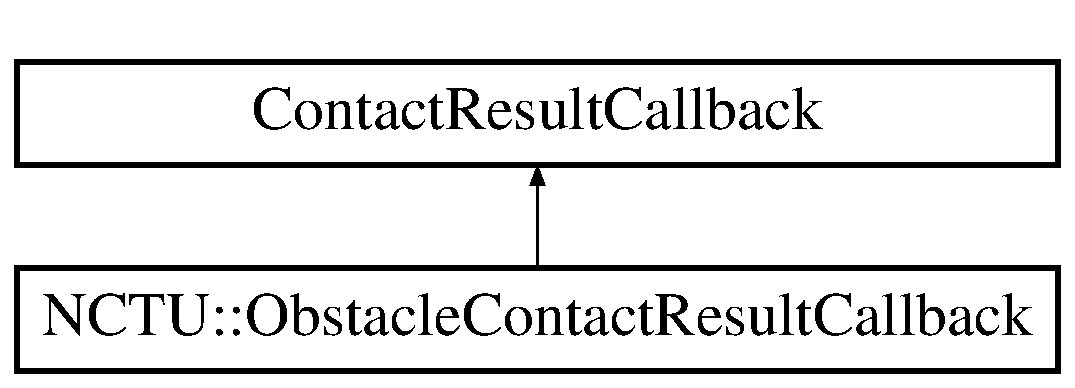
\includegraphics[height=2.000000cm]{struct_n_c_t_u_1_1_obstacle_contact_result_callback}
\end{center}
\end{figure}
\subsection*{Public Member Functions}
\begin{DoxyCompactItemize}
\item 
\hyperlink{struct_n_c_t_u_1_1_obstacle_contact_result_callback_a78326c84bd2641b4d26810491efe6219}{Obstacle\+Contact\+Result\+Callback} (\hyperlink{class_n_c_t_u_1_1_obstacle}{Obstacle} $\ast$ptr)\hypertarget{struct_n_c_t_u_1_1_obstacle_contact_result_callback_a78326c84bd2641b4d26810491efe6219}{}\label{struct_n_c_t_u_1_1_obstacle_contact_result_callback_a78326c84bd2641b4d26810491efe6219}

\begin{DoxyCompactList}\small\item\em handle contact result \end{DoxyCompactList}\item 
bt\+Scalar {\bfseries add\+Single\+Result} (bt\+Manifold\+Point \&cp, const bt\+Collision\+Object\+Wrapper $\ast$col\+Obj0\+Wrap, int part\+Id0, int index0, const bt\+Collision\+Object\+Wrapper $\ast$col\+Obj1\+Wrap, int part\+Id1, int index1)\hypertarget{struct_n_c_t_u_1_1_obstacle_contact_result_callback_af92b627599b6e4751b267d87d55d82fc}{}\label{struct_n_c_t_u_1_1_obstacle_contact_result_callback_af92b627599b6e4751b267d87d55d82fc}

\end{DoxyCompactItemize}
\subsection*{Public Attributes}
\begin{DoxyCompactItemize}
\item 
\hyperlink{class_n_c_t_u_1_1_obstacle}{Obstacle} $\ast$ \hyperlink{struct_n_c_t_u_1_1_obstacle_contact_result_callback_aa14f909b30ebcc73112813427abb554e}{m\+Subject}\hypertarget{struct_n_c_t_u_1_1_obstacle_contact_result_callback_aa14f909b30ebcc73112813427abb554e}{}\label{struct_n_c_t_u_1_1_obstacle_contact_result_callback_aa14f909b30ebcc73112813427abb554e}

\begin{DoxyCompactList}\small\item\em pointer to the subject \end{DoxyCompactList}\end{DoxyCompactItemize}


\subsection{Detailed Description}
callback for player-\/obstalce contact event 

The documentation for this struct was generated from the following files\+:\begin{DoxyCompactItemize}
\item 
N\+C\+T\+U\+Obstacle/include/N\+C\+T\+U\+Obstacle\+Callback.\+h\item 
N\+C\+T\+U\+Obstacle/src/N\+C\+T\+U\+Obstacle\+Callback.\+cpp\end{DoxyCompactItemize}

\hypertarget{class_n_c_t_u_1_1_obstacle_manager}{}\section{N\+C\+TU\+:\+:Obstacle\+Manager Class Reference}
\label{class_n_c_t_u_1_1_obstacle_manager}\index{N\+C\+T\+U\+::\+Obstacle\+Manager@{N\+C\+T\+U\+::\+Obstacle\+Manager}}


obstacle manager  




{\ttfamily \#include $<$N\+C\+T\+U\+Obstacle\+Manager.\+h$>$}

\subsection*{Public Member Functions}
\begin{DoxyCompactItemize}
\item 
\hyperlink{class_n_c_t_u_1_1_obstacle_manager_ada5fb64df1bac37e1f4e9b82769da20d}{Obstacle\+Manager} ()\hypertarget{class_n_c_t_u_1_1_obstacle_manager_ada5fb64df1bac37e1f4e9b82769da20d}{}\label{class_n_c_t_u_1_1_obstacle_manager_ada5fb64df1bac37e1f4e9b82769da20d}

\begin{DoxyCompactList}\small\item\em constructor \end{DoxyCompactList}\item 
\hyperlink{class_n_c_t_u_1_1_obstacle_manager_acaa43e4c78c43cd2c577b3871d292676}{Obstacle\+Manager} (const \hyperlink{class_n_c_t_u_1_1_obstacle_manager}{Obstacle\+Manager} \&)\hypertarget{class_n_c_t_u_1_1_obstacle_manager_acaa43e4c78c43cd2c577b3871d292676}{}\label{class_n_c_t_u_1_1_obstacle_manager_acaa43e4c78c43cd2c577b3871d292676}

\begin{DoxyCompactList}\small\item\em copy constructor \end{DoxyCompactList}\item 
\hyperlink{class_n_c_t_u_1_1_obstacle_manager_a48031a527139901ddfc4d1a9d51ff367}{$\sim$\+Obstacle\+Manager} ()\hypertarget{class_n_c_t_u_1_1_obstacle_manager_a48031a527139901ddfc4d1a9d51ff367}{}\label{class_n_c_t_u_1_1_obstacle_manager_a48031a527139901ddfc4d1a9d51ff367}

\begin{DoxyCompactList}\small\item\em destructor \end{DoxyCompactList}\item 
void \hyperlink{class_n_c_t_u_1_1_obstacle_manager_a798eefd08709801f44285d155e0a5902}{setup} (\hyperlink{class_basic_tutorial__00}{Basic\+Tutorial\+\_\+00} $\ast$app, Ogre\+::\+Scene\+Manager $\ast$, const Ogre\+::\+Axis\+Aligned\+Box \&bound, const Ogre\+::\+Vector3 g)\hypertarget{class_n_c_t_u_1_1_obstacle_manager_a798eefd08709801f44285d155e0a5902}{}\label{class_n_c_t_u_1_1_obstacle_manager_a798eefd08709801f44285d155e0a5902}

\begin{DoxyCompactList}\small\item\em setup the manager \end{DoxyCompactList}\item 
\hyperlink{class_n_c_t_u_1_1_floor_obstacle}{Floor\+Obstacle} $\ast$ \hyperlink{class_n_c_t_u_1_1_obstacle_manager_a01a256af4e1c2daf7393a0efef7762d7}{create\+Floor} (const Ogre\+::\+Vector3 \&normal, Ogre\+::\+Real distance, Ogre\+::\+Real restitution, Ogre\+::\+Real friction)\hypertarget{class_n_c_t_u_1_1_obstacle_manager_a01a256af4e1c2daf7393a0efef7762d7}{}\label{class_n_c_t_u_1_1_obstacle_manager_a01a256af4e1c2daf7393a0efef7762d7}

\begin{DoxyCompactList}\small\item\em create a floor obstacle \end{DoxyCompactList}\item 
\hyperlink{class_n_c_t_u_1_1_floor_obstacle}{Floor\+Obstacle} $\ast$ \hyperlink{class_n_c_t_u_1_1_obstacle_manager_a8ade0023637931e443eea3f5ff173ca9}{create\+Floor} (Ogre\+::\+Plane \&plane, Ogre\+::\+Entity $\ast$entity, Ogre\+::\+Real restitution, Ogre\+::\+Real friction)\hypertarget{class_n_c_t_u_1_1_obstacle_manager_a8ade0023637931e443eea3f5ff173ca9}{}\label{class_n_c_t_u_1_1_obstacle_manager_a8ade0023637931e443eea3f5ff173ca9}

\begin{DoxyCompactList}\small\item\em create a floor obstacle without creating Ogre3D object \end{DoxyCompactList}\item 
\hyperlink{class_n_c_t_u_1_1_player_obstacle}{Player\+Obstacle} $\ast$ \hyperlink{class_n_c_t_u_1_1_obstacle_manager_a684daad777b334deb7fee8e4ac81690b}{create\+Player} (Ogre\+::\+Real restitution, Ogre\+::\+Real friction, Ogre\+::\+Real mass, const Ogre\+::\+String \&name, Ogre\+::\+Vector3 scale=Ogre\+::\+Vector3(50.\+0f, 50.\+0f, 50.\+0f))\hypertarget{class_n_c_t_u_1_1_obstacle_manager_a684daad777b334deb7fee8e4ac81690b}{}\label{class_n_c_t_u_1_1_obstacle_manager_a684daad777b334deb7fee8e4ac81690b}

\begin{DoxyCompactList}\small\item\em create a player obstacle \end{DoxyCompactList}\item 
\hyperlink{class_n_c_t_u_1_1_player_obstacle}{Player\+Obstacle} $\ast$ \hyperlink{class_n_c_t_u_1_1_obstacle_manager_a442ee26a82c9d990a6c1325f56b8ab66}{create\+Player} (Ogre\+::\+Real restitution, Ogre\+::\+Real friction, Ogre\+::\+Real mass, Ogre\+::\+Scene\+Node $\ast$node, Ogre\+::\+Entity $\ast$ent)\hypertarget{class_n_c_t_u_1_1_obstacle_manager_a442ee26a82c9d990a6c1325f56b8ab66}{}\label{class_n_c_t_u_1_1_obstacle_manager_a442ee26a82c9d990a6c1325f56b8ab66}

\begin{DoxyCompactList}\small\item\em create a player obstacle without creating Ogre3D object \end{DoxyCompactList}\item 
\hyperlink{class_n_c_t_u_1_1_cube_obstacle}{Cube\+Obstacle} $\ast$ \hyperlink{class_n_c_t_u_1_1_obstacle_manager_a1a74bbd12d793b3e58535f08553834fa}{create\+Cube} (Ogre\+::\+Real restitution, Ogre\+::\+Real friction, Ogre\+::\+Real mass, const Ogre\+::\+Vector3 \&position, const Ogre\+::\+Vector3 \&size=Ogre\+::\+Vector3\+::\+Z\+E\+RO, const Ogre\+::\+Quaternion \&orientation=Ogre\+::\+Quaternion(0, 0, 0, 1))\hypertarget{class_n_c_t_u_1_1_obstacle_manager_a1a74bbd12d793b3e58535f08553834fa}{}\label{class_n_c_t_u_1_1_obstacle_manager_a1a74bbd12d793b3e58535f08553834fa}

\begin{DoxyCompactList}\small\item\em create a cube obstacle \end{DoxyCompactList}\item 
\hyperlink{class_n_c_t_u_1_1_sphere_obstacle}{Sphere\+Obstacle} $\ast$ \hyperlink{class_n_c_t_u_1_1_obstacle_manager_a00187a4c4360d8ac845b52e24c05ddac}{create\+Sphere} (Ogre\+::\+Real restitution, Ogre\+::\+Real friction, Ogre\+::\+Real mass, const Ogre\+::\+Vector3 \&position, Ogre\+::\+Real radius=1.\+0f, const Ogre\+::\+Quaternion \&orientation=\+Ogre\+::\+Quaternion(0, 0, 0, 1))\hypertarget{class_n_c_t_u_1_1_obstacle_manager_a00187a4c4360d8ac845b52e24c05ddac}{}\label{class_n_c_t_u_1_1_obstacle_manager_a00187a4c4360d8ac845b52e24c05ddac}

\begin{DoxyCompactList}\small\item\em create a sphere obstacle \end{DoxyCompactList}\item 
\hyperlink{class_n_c_t_u_1_1_bullet_obstacle}{Bullet\+Obstacle} $\ast$ \hyperlink{class_n_c_t_u_1_1_obstacle_manager_a38aebf62935a98e585e0b76615229892}{create\+Bullet} (Ogre\+::\+Real restitution, Ogre\+::\+Real friction, Ogre\+::\+Real mass, Hp\+Type bullet\+Type, const Ogre\+::\+Vector3 \&position, Ogre\+::\+Real radius=20.\+0f, const Ogre\+::\+Quaternion \&orientation=\+Ogre\+::\+Quaternion(0, 0, 0, 1))\hypertarget{class_n_c_t_u_1_1_obstacle_manager_a38aebf62935a98e585e0b76615229892}{}\label{class_n_c_t_u_1_1_obstacle_manager_a38aebf62935a98e585e0b76615229892}

\begin{DoxyCompactList}\small\item\em create a bullet obstacle \end{DoxyCompactList}\item 
\hyperlink{class_n_c_t_u_1_1_pickup_obstacle}{Pickup\+Obstacle} $\ast$ \hyperlink{class_n_c_t_u_1_1_obstacle_manager_a9a3da8a738775758a87768146808a3b9}{create\+Pickup} (Ogre\+::\+Scene\+Node $\ast$node, Ogre\+::\+Entity $\ast$ent)\hypertarget{class_n_c_t_u_1_1_obstacle_manager_a9a3da8a738775758a87768146808a3b9}{}\label{class_n_c_t_u_1_1_obstacle_manager_a9a3da8a738775758a87768146808a3b9}

\begin{DoxyCompactList}\small\item\em create a pickup obstacle \end{DoxyCompactList}\item 
\hyperlink{class_n_c_t_u_1_1_general_obstacle}{General\+Obstacle} $\ast$ \hyperlink{class_n_c_t_u_1_1_obstacle_manager_ac0865d03940bcc60aba170a3070def8d}{create\+General\+Obstacle} (Ogre\+::\+Real restitution, Ogre\+::\+Real friction, Ogre\+::\+Real mass, Ogre\+::\+Scene\+Node $\ast$node, Ogre\+::\+Entity $\ast$ent)\hypertarget{class_n_c_t_u_1_1_obstacle_manager_ac0865d03940bcc60aba170a3070def8d}{}\label{class_n_c_t_u_1_1_obstacle_manager_ac0865d03940bcc60aba170a3070def8d}

\begin{DoxyCompactList}\small\item\em create a general obstacle \end{DoxyCompactList}\item 
void \hyperlink{class_n_c_t_u_1_1_obstacle_manager_a9515930be3955052fca23e4826f17565}{set\+Player\+Floor\+Callback} (bt\+Collision\+World\+::\+Contact\+Result\+Callback \&callback)\hypertarget{class_n_c_t_u_1_1_obstacle_manager_a9515930be3955052fca23e4826f17565}{}\label{class_n_c_t_u_1_1_obstacle_manager_a9515930be3955052fca23e4826f17565}

\begin{DoxyCompactList}\small\item\em set player-\/floor callback \end{DoxyCompactList}\item 
void \hyperlink{class_n_c_t_u_1_1_obstacle_manager_adbcd798a63e0ea31250c9cd02ae7c8e0}{set\+Player\+All\+Obstacle\+Callback} (bt\+Collision\+World\+::\+Contact\+Result\+Callback \&callback)\hypertarget{class_n_c_t_u_1_1_obstacle_manager_adbcd798a63e0ea31250c9cd02ae7c8e0}{}\label{class_n_c_t_u_1_1_obstacle_manager_adbcd798a63e0ea31250c9cd02ae7c8e0}

\begin{DoxyCompactList}\small\item\em set player-\/all\+\_\+obstacles callback \end{DoxyCompactList}\item 
void \hyperlink{class_n_c_t_u_1_1_obstacle_manager_abc303dbfc06ae04ab42631806721940e}{update\+Collision} (const Ogre\+::\+Frame\+Event \&evt)\hypertarget{class_n_c_t_u_1_1_obstacle_manager_abc303dbfc06ae04ab42631806721940e}{}\label{class_n_c_t_u_1_1_obstacle_manager_abc303dbfc06ae04ab42631806721940e}

\begin{DoxyCompactList}\small\item\em update collision \end{DoxyCompactList}\item 
void \hyperlink{class_n_c_t_u_1_1_obstacle_manager_a879d568c6f03ca00924e6bca87de1b4e}{update\+Life\+Time} (const Ogre\+::\+Frame\+Event \&evt)\hypertarget{class_n_c_t_u_1_1_obstacle_manager_a879d568c6f03ca00924e6bca87de1b4e}{}\label{class_n_c_t_u_1_1_obstacle_manager_a879d568c6f03ca00924e6bca87de1b4e}

\begin{DoxyCompactList}\small\item\em update life time \end{DoxyCompactList}\item 
void \hyperlink{class_n_c_t_u_1_1_obstacle_manager_a57adf5bc9c6a0fd81f02530b496b8894}{update\+Bullet\+Collision} (const Ogre\+::\+Frame\+Event \&evt)\hypertarget{class_n_c_t_u_1_1_obstacle_manager_a57adf5bc9c6a0fd81f02530b496b8894}{}\label{class_n_c_t_u_1_1_obstacle_manager_a57adf5bc9c6a0fd81f02530b496b8894}

\begin{DoxyCompactList}\small\item\em update bullet collision \end{DoxyCompactList}\item 
void \hyperlink{class_n_c_t_u_1_1_obstacle_manager_a9db096654d7779d29fc7e584a63c6a88}{update\+Player\+Pickups\+Collision} (const Ogre\+::\+Frame\+Event \&evt)\hypertarget{class_n_c_t_u_1_1_obstacle_manager_a9db096654d7779d29fc7e584a63c6a88}{}\label{class_n_c_t_u_1_1_obstacle_manager_a9db096654d7779d29fc7e584a63c6a88}

\begin{DoxyCompactList}\small\item\em update player-\/pickups collision \end{DoxyCompactList}\item 
void \hyperlink{class_n_c_t_u_1_1_obstacle_manager_ad8539bf73bdce5499fd43aacbe1aef96}{update\+Pickups\+Effects} (const Ogre\+::\+Frame\+Event \&evt)\hypertarget{class_n_c_t_u_1_1_obstacle_manager_ad8539bf73bdce5499fd43aacbe1aef96}{}\label{class_n_c_t_u_1_1_obstacle_manager_ad8539bf73bdce5499fd43aacbe1aef96}

\begin{DoxyCompactList}\small\item\em update pickup effect \end{DoxyCompactList}\item 
Ogre\+Bullet\+Dynamics\+::\+Dynamics\+World $\ast$ \hyperlink{class_n_c_t_u_1_1_obstacle_manager_aed73f2c32c6e2c728b7152162770c95a}{get\+World} ()\hypertarget{class_n_c_t_u_1_1_obstacle_manager_aed73f2c32c6e2c728b7152162770c95a}{}\label{class_n_c_t_u_1_1_obstacle_manager_aed73f2c32c6e2c728b7152162770c95a}

\begin{DoxyCompactList}\small\item\em get the bullet world pointer \end{DoxyCompactList}\item 
Ogre\+::\+Scene\+Manager $\ast$ \hyperlink{class_n_c_t_u_1_1_obstacle_manager_a6c51f824cbbfd4ed12edd855af65aac9}{get\+Scene\+Mgr} ()\hypertarget{class_n_c_t_u_1_1_obstacle_manager_a6c51f824cbbfd4ed12edd855af65aac9}{}\label{class_n_c_t_u_1_1_obstacle_manager_a6c51f824cbbfd4ed12edd855af65aac9}

\begin{DoxyCompactList}\small\item\em get the scene manager pointer \end{DoxyCompactList}\item 
\hyperlink{class_n_c_t_u_1_1_player_obstacle}{Player\+Obstacle} $\ast$ \hyperlink{class_n_c_t_u_1_1_obstacle_manager_ade1d39349279aec3da7e86a21c9c5078}{get\+Player} ()\hypertarget{class_n_c_t_u_1_1_obstacle_manager_ade1d39349279aec3da7e86a21c9c5078}{}\label{class_n_c_t_u_1_1_obstacle_manager_ade1d39349279aec3da7e86a21c9c5078}

\begin{DoxyCompactList}\small\item\em get the player obstacle pointer \end{DoxyCompactList}\item 
\hyperlink{class_n_c_t_u_1_1_floor_obstacle}{Floor\+Obstacle} $\ast$ \hyperlink{class_n_c_t_u_1_1_obstacle_manager_a1f8902cb64c36022a8096b455f6e8967}{get\+Floor} ()\hypertarget{class_n_c_t_u_1_1_obstacle_manager_a1f8902cb64c36022a8096b455f6e8967}{}\label{class_n_c_t_u_1_1_obstacle_manager_a1f8902cb64c36022a8096b455f6e8967}

\begin{DoxyCompactList}\small\item\em get the floor obstacle pointer \end{DoxyCompactList}\item 
\hyperlink{class_basic_tutorial__00}{Basic\+Tutorial\+\_\+00} $\ast$ \hyperlink{class_n_c_t_u_1_1_obstacle_manager_a879ce2bab22ebc1d4ed510f56cc13f7e}{get\+App} ()\hypertarget{class_n_c_t_u_1_1_obstacle_manager_a879ce2bab22ebc1d4ed510f56cc13f7e}{}\label{class_n_c_t_u_1_1_obstacle_manager_a879ce2bab22ebc1d4ed510f56cc13f7e}

\begin{DoxyCompactList}\small\item\em get the pointer to the application \end{DoxyCompactList}\item 
void \hyperlink{class_n_c_t_u_1_1_obstacle_manager_a274b9d85c938b325fba41129ecb5e9ba}{step\+Simulation} (Ogre\+::\+Real time)\hypertarget{class_n_c_t_u_1_1_obstacle_manager_a274b9d85c938b325fba41129ecb5e9ba}{}\label{class_n_c_t_u_1_1_obstacle_manager_a274b9d85c938b325fba41129ecb5e9ba}

\begin{DoxyCompactList}\small\item\em step the simulation for physics \end{DoxyCompactList}\item 
void \hyperlink{class_n_c_t_u_1_1_obstacle_manager_aacd7dbd0b2c851691d1f36582d7779dd}{remove\+Player\+Obstacle} ()\hypertarget{class_n_c_t_u_1_1_obstacle_manager_aacd7dbd0b2c851691d1f36582d7779dd}{}\label{class_n_c_t_u_1_1_obstacle_manager_aacd7dbd0b2c851691d1f36582d7779dd}

\begin{DoxyCompactList}\small\item\em remove the player obstacle \end{DoxyCompactList}\item 
void \hyperlink{class_n_c_t_u_1_1_obstacle_manager_a5c37bc1f270352a9df4c0e95642ff51d}{remove\+Floor\+Obstacle} ()\hypertarget{class_n_c_t_u_1_1_obstacle_manager_a5c37bc1f270352a9df4c0e95642ff51d}{}\label{class_n_c_t_u_1_1_obstacle_manager_a5c37bc1f270352a9df4c0e95642ff51d}

\begin{DoxyCompactList}\small\item\em remove the floor obstacle \end{DoxyCompactList}\item 
void \hyperlink{class_n_c_t_u_1_1_obstacle_manager_abe8ff3d60b7953e8540953882646a652}{remove\+All\+Obstacles} ()\hypertarget{class_n_c_t_u_1_1_obstacle_manager_abe8ff3d60b7953e8540953882646a652}{}\label{class_n_c_t_u_1_1_obstacle_manager_abe8ff3d60b7953e8540953882646a652}

\begin{DoxyCompactList}\small\item\em remove all obstacle \end{DoxyCompactList}\item 
std\+::list$<$ \hyperlink{class_n_c_t_u_1_1_obstacle}{Obstacle} $\ast$ $>$\+::iterator \hyperlink{class_n_c_t_u_1_1_obstacle_manager_a260911f02f5425bf9f22973bcc065a42}{delete\+By\+Iterator} (std\+::list$<$ \hyperlink{class_n_c_t_u_1_1_obstacle}{Obstacle} $\ast$ $>$\+::iterator it)\hypertarget{class_n_c_t_u_1_1_obstacle_manager_a260911f02f5425bf9f22973bcc065a42}{}\label{class_n_c_t_u_1_1_obstacle_manager_a260911f02f5425bf9f22973bcc065a42}

\begin{DoxyCompactList}\small\item\em delete obstacle by iterator \end{DoxyCompactList}\item 
std\+::list$<$ \hyperlink{class_n_c_t_u_1_1_bullet_obstacle}{Bullet\+Obstacle} $\ast$ $>$\+::iterator \hyperlink{class_n_c_t_u_1_1_obstacle_manager_a6ee337af765406950207541982ea0f73}{remove\+Bullet\+Iterator} (std\+::list$<$ \hyperlink{class_n_c_t_u_1_1_bullet_obstacle}{Bullet\+Obstacle} $\ast$ $>$\+::iterator it)\hypertarget{class_n_c_t_u_1_1_obstacle_manager_a6ee337af765406950207541982ea0f73}{}\label{class_n_c_t_u_1_1_obstacle_manager_a6ee337af765406950207541982ea0f73}

\begin{DoxyCompactList}\small\item\em delete bullet by iterator \end{DoxyCompactList}\item 
std\+::list$<$ \hyperlink{class_n_c_t_u_1_1_pickup_obstacle}{Pickup\+Obstacle} $\ast$ $>$\+::iterator \hyperlink{class_n_c_t_u_1_1_obstacle_manager_a7c35359f1c719429a88350db867ce72e}{remove\+Pickup\+Iterator} (std\+::list$<$ \hyperlink{class_n_c_t_u_1_1_pickup_obstacle}{Pickup\+Obstacle} $\ast$ $>$\+::iterator it)\hypertarget{class_n_c_t_u_1_1_obstacle_manager_a7c35359f1c719429a88350db867ce72e}{}\label{class_n_c_t_u_1_1_obstacle_manager_a7c35359f1c719429a88350db867ce72e}

\begin{DoxyCompactList}\small\item\em delete pickup by iterator \end{DoxyCompactList}\end{DoxyCompactItemize}
\subsection*{Public Attributes}
\begin{DoxyCompactItemize}
\item 
Score\+Handler \hyperlink{class_n_c_t_u_1_1_obstacle_manager_ae1e85963f99511e675c81261681131e4}{m\+Score\+Handler}\hypertarget{class_n_c_t_u_1_1_obstacle_manager_ae1e85963f99511e675c81261681131e4}{}\label{class_n_c_t_u_1_1_obstacle_manager_ae1e85963f99511e675c81261681131e4}

\begin{DoxyCompactList}\small\item\em the score handler \end{DoxyCompactList}\end{DoxyCompactItemize}


\subsection{Detailed Description}
obstacle manager 

The documentation for this class was generated from the following files\+:\begin{DoxyCompactItemize}
\item 
N\+C\+T\+U\+Obstacle/include/N\+C\+T\+U\+Obstacle\+Manager.\+h\item 
N\+C\+T\+U\+Obstacle/src/N\+C\+T\+U\+Obstacle\+Manager.\+cpp\end{DoxyCompactItemize}

\hypertarget{class_ogre_1_1_obstacle_property}{}\section{Ogre\+:\+:Obstacle\+Property Class Reference}
\label{class_ogre_1_1_obstacle_property}\index{Ogre\+::\+Obstacle\+Property@{Ogre\+::\+Obstacle\+Property}}


store properties for a obstacle  




{\ttfamily \#include $<$Dot\+Scene\+Loader.\+h$>$}

\subsection*{Public Member Functions}
\begin{DoxyCompactItemize}
\item 
\hyperlink{class_ogre_1_1_obstacle_property_a3fdadc88931b0d7d475cafea2936c157}{Obstacle\+Property} ()\hypertarget{class_ogre_1_1_obstacle_property_a3fdadc88931b0d7d475cafea2936c157}{}\label{class_ogre_1_1_obstacle_property_a3fdadc88931b0d7d475cafea2936c157}

\begin{DoxyCompactList}\small\item\em constructor \end{DoxyCompactList}\end{DoxyCompactItemize}
\subsection*{Public Attributes}
\begin{DoxyCompactItemize}
\item 
String \hyperlink{class_ogre_1_1_obstacle_property_acb12c59bd4a980cc4c975efd92820257}{obstacle\+\_\+type}\hypertarget{class_ogre_1_1_obstacle_property_acb12c59bd4a980cc4c975efd92820257}{}\label{class_ogre_1_1_obstacle_property_acb12c59bd4a980cc4c975efd92820257}

\begin{DoxyCompactList}\small\item\em type of obstacle \end{DoxyCompactList}\item 
Real \hyperlink{class_ogre_1_1_obstacle_property_acde56ca0142762faf2e63b6e8d836ee0}{mass}\hypertarget{class_ogre_1_1_obstacle_property_acde56ca0142762faf2e63b6e8d836ee0}{}\label{class_ogre_1_1_obstacle_property_acde56ca0142762faf2e63b6e8d836ee0}

\begin{DoxyCompactList}\small\item\em mass for physics \end{DoxyCompactList}\item 
Real \hyperlink{class_ogre_1_1_obstacle_property_adb0760a89f43b1edbcbf2af2a8fe24b1}{friction}\hypertarget{class_ogre_1_1_obstacle_property_adb0760a89f43b1edbcbf2af2a8fe24b1}{}\label{class_ogre_1_1_obstacle_property_adb0760a89f43b1edbcbf2af2a8fe24b1}

\begin{DoxyCompactList}\small\item\em friction for physics \end{DoxyCompactList}\item 
Real \hyperlink{class_ogre_1_1_obstacle_property_a3d31e025db70452296eedd9d862c713f}{restitution}\hypertarget{class_ogre_1_1_obstacle_property_a3d31e025db70452296eedd9d862c713f}{}\label{class_ogre_1_1_obstacle_property_a3d31e025db70452296eedd9d862c713f}

\begin{DoxyCompactList}\small\item\em restitution for physics \end{DoxyCompactList}\item 
int \hyperlink{class_ogre_1_1_obstacle_property_af68da2cebce6ab8bc5259be36a607885}{hit\+Point}\hypertarget{class_ogre_1_1_obstacle_property_af68da2cebce6ab8bc5259be36a607885}{}\label{class_ogre_1_1_obstacle_property_af68da2cebce6ab8bc5259be36a607885}

\begin{DoxyCompactList}\small\item\em hit point of this obstacle \end{DoxyCompactList}\item 
N\+C\+T\+U\+::\+Hp\+Type \hyperlink{class_ogre_1_1_obstacle_property_a61d0e36adb78beb9b4a6a6022b0e867c}{hp\+Type}\hypertarget{class_ogre_1_1_obstacle_property_a61d0e36adb78beb9b4a6a6022b0e867c}{}\label{class_ogre_1_1_obstacle_property_a61d0e36adb78beb9b4a6a6022b0e867c}

\begin{DoxyCompactList}\small\item\em type of hit point(\+H\+P) \end{DoxyCompactList}\item 
Real \hyperlink{class_ogre_1_1_obstacle_property_abf521aa3acbf7f824449f67ed8d631e2}{bump\+Speed}\hypertarget{class_ogre_1_1_obstacle_property_abf521aa3acbf7f824449f67ed8d631e2}{}\label{class_ogre_1_1_obstacle_property_abf521aa3acbf7f824449f67ed8d631e2}

\begin{DoxyCompactList}\small\item\em speed for bumping bed \end{DoxyCompactList}\item 
String \hyperlink{class_ogre_1_1_obstacle_property_a669e6b77766ce91fc971002b739992d6}{turn\+Type}\hypertarget{class_ogre_1_1_obstacle_property_a669e6b77766ce91fc971002b739992d6}{}\label{class_ogre_1_1_obstacle_property_a669e6b77766ce91fc971002b739992d6}

\begin{DoxyCompactList}\small\item\em turn type (left or right) for turing plane \end{DoxyCompactList}\item 
std\+::deque$<$ std\+::pair$<$ Ogre\+::\+Vector3, Ogre\+::\+Real $>$ $>$ \hyperlink{class_ogre_1_1_obstacle_property_a6732ff592c84b16e7b191974be9f7cbf}{condition\+Vectors}\hypertarget{class_ogre_1_1_obstacle_property_a6732ff592c84b16e7b191974be9f7cbf}{}\label{class_ogre_1_1_obstacle_property_a6732ff592c84b16e7b191974be9f7cbf}

\begin{DoxyCompactList}\small\item\em lots of condition vectors \end{DoxyCompactList}\item 
\hyperlink{classprop_map}{prop\+Map}$<$ int, String $>$ \hyperlink{class_ogre_1_1_obstacle_property_ad434aeef04327df2282521d74845b309}{hp\+Change\+Materials}\hypertarget{class_ogre_1_1_obstacle_property_ad434aeef04327df2282521d74845b309}{}\label{class_ogre_1_1_obstacle_property_ad434aeef04327df2282521d74845b309}

\begin{DoxyCompactList}\small\item\em material names for different hp point \end{DoxyCompactList}\end{DoxyCompactItemize}


\subsection{Detailed Description}
store properties for a obstacle 

The documentation for this class was generated from the following file\+:\begin{DoxyCompactItemize}
\item 
programs/\+Obstacle/include/Dot\+Scene\+Loader.\+h\end{DoxyCompactItemize}

\hypertarget{struct_n_c_t_u_1_1_particle_system_pack}{}\section{N\+C\+TU\+:\+:Particle\+System\+Pack Struct Reference}
\label{struct_n_c_t_u_1_1_particle_system_pack}\index{N\+C\+T\+U\+::\+Particle\+System\+Pack@{N\+C\+T\+U\+::\+Particle\+System\+Pack}}


a pack of particle system variables  




{\ttfamily \#include $<$N\+C\+T\+U\+Obstacle.\+h$>$}

\subsection*{Public Member Functions}
\begin{DoxyCompactItemize}
\item 
\hyperlink{struct_n_c_t_u_1_1_particle_system_pack_a16f7b382e0147aec37d65597443624f5}{Particle\+System\+Pack} ()\hypertarget{struct_n_c_t_u_1_1_particle_system_pack_a16f7b382e0147aec37d65597443624f5}{}\label{struct_n_c_t_u_1_1_particle_system_pack_a16f7b382e0147aec37d65597443624f5}

\begin{DoxyCompactList}\small\item\em constructor \end{DoxyCompactList}\end{DoxyCompactItemize}
\subsection*{Public Attributes}
\begin{DoxyCompactItemize}
\item 
bool \hyperlink{struct_n_c_t_u_1_1_particle_system_pack_af7a913d5790d6ad7e5a4cc95f0b990bd}{m\+Particle\+System\+Init}\hypertarget{struct_n_c_t_u_1_1_particle_system_pack_af7a913d5790d6ad7e5a4cc95f0b990bd}{}\label{struct_n_c_t_u_1_1_particle_system_pack_af7a913d5790d6ad7e5a4cc95f0b990bd}

\begin{DoxyCompactList}\small\item\em is the particle system initailized? \end{DoxyCompactList}\item 
Ogre\+::\+Scene\+Node $\ast$ \hyperlink{struct_n_c_t_u_1_1_particle_system_pack_ac49856e3bda9706e29a2631b437683ea}{m\+Particle\+System\+Node}\hypertarget{struct_n_c_t_u_1_1_particle_system_pack_ac49856e3bda9706e29a2631b437683ea}{}\label{struct_n_c_t_u_1_1_particle_system_pack_ac49856e3bda9706e29a2631b437683ea}

\begin{DoxyCompactList}\small\item\em the pointer to the particle system scene node \end{DoxyCompactList}\item 
Ogre\+::\+Particle\+System $\ast$ \hyperlink{struct_n_c_t_u_1_1_particle_system_pack_ab9d8cc21e547221dafc5aafb7c1cc3b3}{m\+Particle\+System}\hypertarget{struct_n_c_t_u_1_1_particle_system_pack_ab9d8cc21e547221dafc5aafb7c1cc3b3}{}\label{struct_n_c_t_u_1_1_particle_system_pack_ab9d8cc21e547221dafc5aafb7c1cc3b3}

\begin{DoxyCompactList}\small\item\em the pointer to the particle system \end{DoxyCompactList}\item 
Ogre\+::\+String \hyperlink{struct_n_c_t_u_1_1_particle_system_pack_ac392bc14df3134eaa6c0a2fe705d80e1}{m\+Particle\+System\+Name}\hypertarget{struct_n_c_t_u_1_1_particle_system_pack_ac392bc14df3134eaa6c0a2fe705d80e1}{}\label{struct_n_c_t_u_1_1_particle_system_pack_ac392bc14df3134eaa6c0a2fe705d80e1}

\begin{DoxyCompactList}\small\item\em name of particle system \end{DoxyCompactList}\end{DoxyCompactItemize}


\subsection{Detailed Description}
a pack of particle system variables 

The documentation for this struct was generated from the following file\+:\begin{DoxyCompactItemize}
\item 
N\+C\+T\+U\+Obstacle/include/N\+C\+T\+U\+Obstacle.\+h\end{DoxyCompactItemize}

\hypertarget{struct_n_c_t_u_1_1_pickup_contact_result_callback}{}\section{N\+C\+TU\+:\+:Pickup\+Contact\+Result\+Callback Struct Reference}
\label{struct_n_c_t_u_1_1_pickup_contact_result_callback}\index{N\+C\+T\+U\+::\+Pickup\+Contact\+Result\+Callback@{N\+C\+T\+U\+::\+Pickup\+Contact\+Result\+Callback}}


callback for player-\/pickup contact  




{\ttfamily \#include $<$N\+C\+T\+U\+Obstacle\+Callback.\+h$>$}

Inheritance diagram for N\+C\+TU\+:\+:Pickup\+Contact\+Result\+Callback\+:\begin{figure}[H]
\begin{center}
\leavevmode
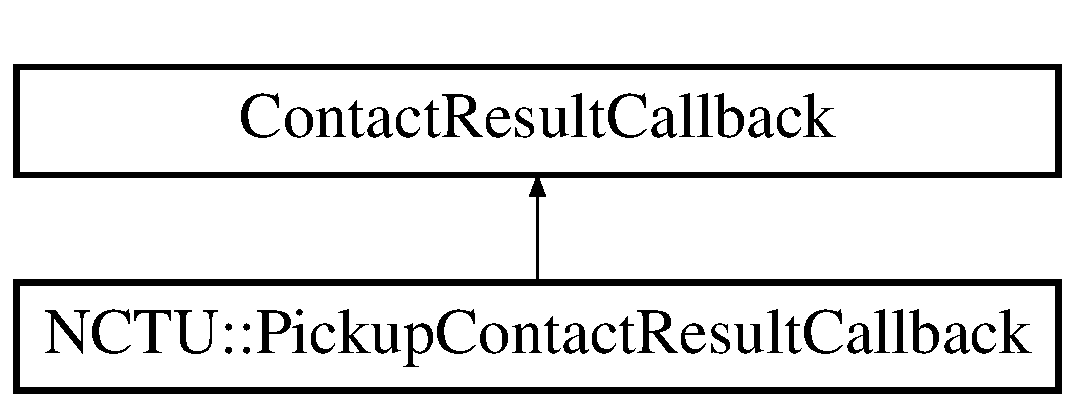
\includegraphics[height=2.000000cm]{struct_n_c_t_u_1_1_pickup_contact_result_callback}
\end{center}
\end{figure}
\subsection*{Public Member Functions}
\begin{DoxyCompactItemize}
\item 
\hyperlink{struct_n_c_t_u_1_1_pickup_contact_result_callback_a3e8d27c4845c0472728072d79e2b7c18}{Pickup\+Contact\+Result\+Callback} (\hyperlink{class_n_c_t_u_1_1_player_obstacle}{Player\+Obstacle} $\ast$me, \hyperlink{class_n_c_t_u_1_1_pickup_obstacle}{Pickup\+Obstacle} $\ast$tgr)\hypertarget{struct_n_c_t_u_1_1_pickup_contact_result_callback_a3e8d27c4845c0472728072d79e2b7c18}{}\label{struct_n_c_t_u_1_1_pickup_contact_result_callback_a3e8d27c4845c0472728072d79e2b7c18}

\begin{DoxyCompactList}\small\item\em handle contact result \end{DoxyCompactList}\item 
bt\+Scalar {\bfseries add\+Single\+Result} (bt\+Manifold\+Point \&cp, const bt\+Collision\+Object\+Wrapper $\ast$col\+Obj0\+Wrap, int part\+Id0, int index0, const bt\+Collision\+Object\+Wrapper $\ast$col\+Obj1\+Wrap, int part\+Id1, int index1)\hypertarget{struct_n_c_t_u_1_1_pickup_contact_result_callback_af517d6df2bca3cfaa30a30953a2d8e74}{}\label{struct_n_c_t_u_1_1_pickup_contact_result_callback_af517d6df2bca3cfaa30a30953a2d8e74}

\end{DoxyCompactItemize}
\subsection*{Public Attributes}
\begin{DoxyCompactItemize}
\item 
\hyperlink{class_n_c_t_u_1_1_pickup_obstacle}{Pickup\+Obstacle} $\ast$ \hyperlink{struct_n_c_t_u_1_1_pickup_contact_result_callback_ab8d5fdde1da18a6552b956223dabae4a}{m\+Object}\hypertarget{struct_n_c_t_u_1_1_pickup_contact_result_callback_ab8d5fdde1da18a6552b956223dabae4a}{}\label{struct_n_c_t_u_1_1_pickup_contact_result_callback_ab8d5fdde1da18a6552b956223dabae4a}

\begin{DoxyCompactList}\small\item\em pointer to the pickup \end{DoxyCompactList}\item 
\hyperlink{class_n_c_t_u_1_1_player_obstacle}{Player\+Obstacle} $\ast$ \hyperlink{struct_n_c_t_u_1_1_pickup_contact_result_callback_a132213ea28df353bdbf5d7cfb55a8d3d}{m\+Subject}\hypertarget{struct_n_c_t_u_1_1_pickup_contact_result_callback_a132213ea28df353bdbf5d7cfb55a8d3d}{}\label{struct_n_c_t_u_1_1_pickup_contact_result_callback_a132213ea28df353bdbf5d7cfb55a8d3d}

\begin{DoxyCompactList}\small\item\em pointer to the player \end{DoxyCompactList}\end{DoxyCompactItemize}


\subsection{Detailed Description}
callback for player-\/pickup contact 

The documentation for this struct was generated from the following files\+:\begin{DoxyCompactItemize}
\item 
N\+C\+T\+U\+Obstacle/include/N\+C\+T\+U\+Obstacle\+Callback.\+h\item 
N\+C\+T\+U\+Obstacle/src/N\+C\+T\+U\+Obstacle\+Callback.\+cpp\end{DoxyCompactItemize}

\hypertarget{class_n_c_t_u_1_1_pickup_obstacle}{}\section{N\+C\+TU\+:\+:Pickup\+Obstacle Class Reference}
\label{class_n_c_t_u_1_1_pickup_obstacle}\index{N\+C\+T\+U\+::\+Pickup\+Obstacle@{N\+C\+T\+U\+::\+Pickup\+Obstacle}}


pickup obstacle  




{\ttfamily \#include $<$N\+C\+T\+U\+Pickup\+Obstacle.\+h$>$}

Inheritance diagram for N\+C\+TU\+:\+:Pickup\+Obstacle\+:\begin{figure}[H]
\begin{center}
\leavevmode
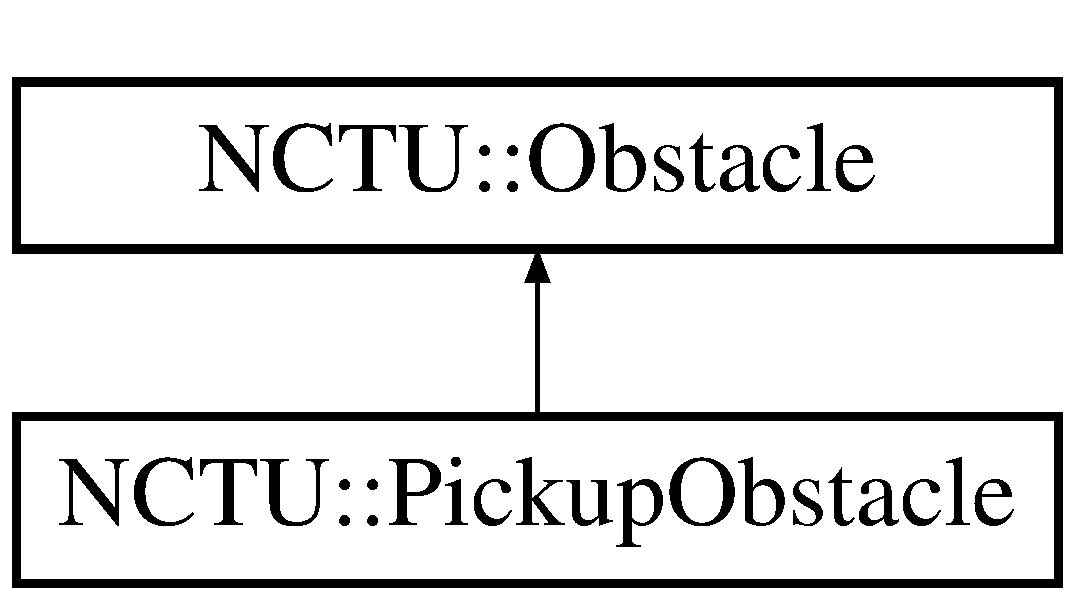
\includegraphics[height=2.000000cm]{class_n_c_t_u_1_1_pickup_obstacle}
\end{center}
\end{figure}
\subsection*{Public Member Functions}
\begin{DoxyCompactItemize}
\item 
\hyperlink{class_n_c_t_u_1_1_pickup_obstacle_a59a11ebd318b216a4b3562b6a78cd5cf}{Pickup\+Obstacle} (\hyperlink{class_n_c_t_u_1_1_obstacle_manager}{Obstacle\+Manager} $\ast$mgmt, I\+N\+D\+E\+X\+\_\+\+T\+Y\+PE index, Ogre\+::\+Scene\+Node $\ast$node, Ogre\+::\+Entity $\ast$ent)\hypertarget{class_n_c_t_u_1_1_pickup_obstacle_a59a11ebd318b216a4b3562b6a78cd5cf}{}\label{class_n_c_t_u_1_1_pickup_obstacle_a59a11ebd318b216a4b3562b6a78cd5cf}

\begin{DoxyCompactList}\small\item\em constructor \end{DoxyCompactList}\item 
virtual void \hyperlink{class_n_c_t_u_1_1_pickup_obstacle_a4748f76158d2cac05d0aeecac10e6910}{set\+Pickup\+Iterator} (std\+::list$<$ \hyperlink{class_n_c_t_u_1_1_pickup_obstacle}{Pickup\+Obstacle} $\ast$ $>$\+::iterator it)\hypertarget{class_n_c_t_u_1_1_pickup_obstacle_a4748f76158d2cac05d0aeecac10e6910}{}\label{class_n_c_t_u_1_1_pickup_obstacle_a4748f76158d2cac05d0aeecac10e6910}

\begin{DoxyCompactList}\small\item\em set pickup iterator for manager \end{DoxyCompactList}\item 
virtual void \hyperlink{class_n_c_t_u_1_1_pickup_obstacle_a27afa507fc666bc80387be4cb75bc49a}{clean\+Up} ()\hypertarget{class_n_c_t_u_1_1_pickup_obstacle_a27afa507fc666bc80387be4cb75bc49a}{}\label{class_n_c_t_u_1_1_pickup_obstacle_a27afa507fc666bc80387be4cb75bc49a}

\begin{DoxyCompactList}\small\item\em clean up routing \end{DoxyCompactList}\item 
virtual bool \hyperlink{class_n_c_t_u_1_1_pickup_obstacle_aab9989c60aa142b509846608207622d9}{can\+Be\+Shoot} () const \hypertarget{class_n_c_t_u_1_1_pickup_obstacle_aab9989c60aa142b509846608207622d9}{}\label{class_n_c_t_u_1_1_pickup_obstacle_aab9989c60aa142b509846608207622d9}

\begin{DoxyCompactList}\small\item\em is this object can be shoot? \end{DoxyCompactList}\item 
virtual bool \hyperlink{class_n_c_t_u_1_1_pickup_obstacle_a4bfe9e56a0793947a464a42dc5286de3}{can\+Stand\+On} () const \hypertarget{class_n_c_t_u_1_1_pickup_obstacle_a4bfe9e56a0793947a464a42dc5286de3}{}\label{class_n_c_t_u_1_1_pickup_obstacle_a4bfe9e56a0793947a464a42dc5286de3}

\begin{DoxyCompactList}\small\item\em is this object can be standed on? \end{DoxyCompactList}\item 
virtual bool \hyperlink{class_n_c_t_u_1_1_pickup_obstacle_acef3668c5a562f6f18d248f418860d96}{can\+Cause\+Dead} () const \hypertarget{class_n_c_t_u_1_1_pickup_obstacle_acef3668c5a562f6f18d248f418860d96}{}\label{class_n_c_t_u_1_1_pickup_obstacle_acef3668c5a562f6f18d248f418860d96}

\begin{DoxyCompactList}\small\item\em is this object can cause dead? \end{DoxyCompactList}\item 
virtual void \hyperlink{class_n_c_t_u_1_1_pickup_obstacle_af4c760c60513ae7baebf0cdc9c15b9f1}{update\+Effect} (const Ogre\+::\+Frame\+Event \&evt)\hypertarget{class_n_c_t_u_1_1_pickup_obstacle_af4c760c60513ae7baebf0cdc9c15b9f1}{}\label{class_n_c_t_u_1_1_pickup_obstacle_af4c760c60513ae7baebf0cdc9c15b9f1}

\begin{DoxyCompactList}\small\item\em update the effect \end{DoxyCompactList}\end{DoxyCompactItemize}
\subsection*{Protected Attributes}
\begin{DoxyCompactItemize}
\item 
I\+N\+D\+E\+X\+\_\+\+T\+Y\+PE \hyperlink{class_n_c_t_u_1_1_pickup_obstacle_aa0886165088dcface28d35cf1b52f73a}{m\+Index}\hypertarget{class_n_c_t_u_1_1_pickup_obstacle_aa0886165088dcface28d35cf1b52f73a}{}\label{class_n_c_t_u_1_1_pickup_obstacle_aa0886165088dcface28d35cf1b52f73a}

\begin{DoxyCompactList}\small\item\em object index \end{DoxyCompactList}\item 
std\+::list$<$ \hyperlink{class_n_c_t_u_1_1_pickup_obstacle}{Pickup\+Obstacle} $\ast$ $>$\+::iterator \hyperlink{class_n_c_t_u_1_1_pickup_obstacle_aac1104c755a32023cbceabcb0385de33}{m\+Pickup\+Iterator}\hypertarget{class_n_c_t_u_1_1_pickup_obstacle_aac1104c755a32023cbceabcb0385de33}{}\label{class_n_c_t_u_1_1_pickup_obstacle_aac1104c755a32023cbceabcb0385de33}

\begin{DoxyCompactList}\small\item\em iterator for manager \end{DoxyCompactList}\end{DoxyCompactItemize}
\subsection*{Additional Inherited Members}


\subsection{Detailed Description}
pickup obstacle 

The documentation for this class was generated from the following files\+:\begin{DoxyCompactItemize}
\item 
N\+C\+T\+U\+Obstacle/include/N\+C\+T\+U\+Pickup\+Obstacle.\+h\item 
N\+C\+T\+U\+Obstacle/src/N\+C\+T\+U\+Pickup\+Obstacle.\+cpp\end{DoxyCompactItemize}

\hypertarget{class_n_c_t_u_1_1_player_obstacle}{}\section{N\+C\+TU\+:\+:Player\+Obstacle Class Reference}
\label{class_n_c_t_u_1_1_player_obstacle}\index{N\+C\+T\+U\+::\+Player\+Obstacle@{N\+C\+T\+U\+::\+Player\+Obstacle}}


player obstacle  




{\ttfamily \#include $<$N\+C\+T\+U\+Player\+Obstacle.\+h$>$}

Inheritance diagram for N\+C\+TU\+:\+:Player\+Obstacle\+:\begin{figure}[H]
\begin{center}
\leavevmode
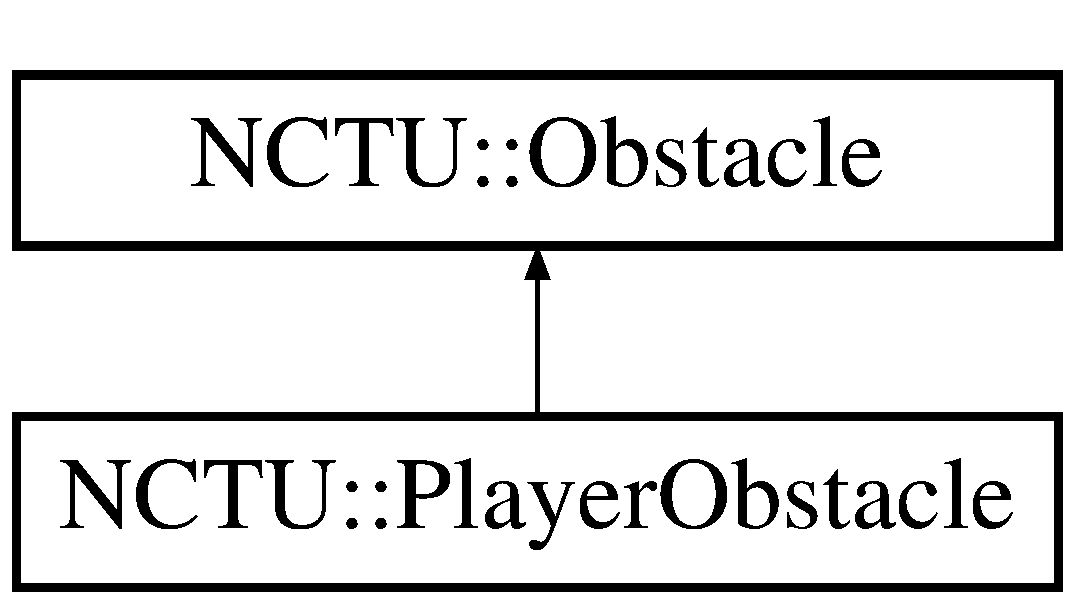
\includegraphics[height=2.000000cm]{class_n_c_t_u_1_1_player_obstacle}
\end{center}
\end{figure}
\subsection*{Public Member Functions}
\begin{DoxyCompactItemize}
\item 
\hyperlink{class_n_c_t_u_1_1_player_obstacle_a983a5de655a8b5aefcae4ae295b68bb5}{Player\+Obstacle} (\hyperlink{class_n_c_t_u_1_1_obstacle_manager}{Obstacle\+Manager} $\ast$mgmt, Ogre\+::\+Real restitution, Ogre\+::\+Real friction, Ogre\+::\+Real mass, const Ogre\+::\+String \&name, Ogre\+::\+Vector3 scale)\hypertarget{class_n_c_t_u_1_1_player_obstacle_a983a5de655a8b5aefcae4ae295b68bb5}{}\label{class_n_c_t_u_1_1_player_obstacle_a983a5de655a8b5aefcae4ae295b68bb5}

\begin{DoxyCompactList}\small\item\em constructor \end{DoxyCompactList}\item 
\hyperlink{class_n_c_t_u_1_1_player_obstacle_aa5fd634767396aeb5c2a8c26931de7bb}{Player\+Obstacle} (\hyperlink{class_n_c_t_u_1_1_obstacle_manager}{Obstacle\+Manager} $\ast$mgmt, Ogre\+::\+Real restitution, Ogre\+::\+Real friction, Ogre\+::\+Real mass, Ogre\+::\+Scene\+Node $\ast$node, Ogre\+::\+Entity $\ast$ent)\hypertarget{class_n_c_t_u_1_1_player_obstacle_aa5fd634767396aeb5c2a8c26931de7bb}{}\label{class_n_c_t_u_1_1_player_obstacle_aa5fd634767396aeb5c2a8c26931de7bb}

\begin{DoxyCompactList}\small\item\em another constructor, but not create scene node and entity \end{DoxyCompactList}\item 
virtual \hyperlink{class_n_c_t_u_1_1_player_obstacle_a6e1139ba9e43ed6158103ff215e25cd8}{$\sim$\+Player\+Obstacle} ()\hypertarget{class_n_c_t_u_1_1_player_obstacle_a6e1139ba9e43ed6158103ff215e25cd8}{}\label{class_n_c_t_u_1_1_player_obstacle_a6e1139ba9e43ed6158103ff215e25cd8}

\begin{DoxyCompactList}\small\item\em destructor \end{DoxyCompactList}\item 
virtual void \hyperlink{class_n_c_t_u_1_1_player_obstacle_a91a946ed66165c94c7cc913b6a9cfe3f}{detach\+Entity} ()\hypertarget{class_n_c_t_u_1_1_player_obstacle_a91a946ed66165c94c7cc913b6a9cfe3f}{}\label{class_n_c_t_u_1_1_player_obstacle_a91a946ed66165c94c7cc913b6a9cfe3f}

\begin{DoxyCompactList}\small\item\em detach entity from scene node \end{DoxyCompactList}\item 
virtual void \hyperlink{class_n_c_t_u_1_1_player_obstacle_a981883a7b5e6e74b5b95f782710ca46c}{set\+Sliding} (bool val)\hypertarget{class_n_c_t_u_1_1_player_obstacle_a981883a7b5e6e74b5b95f782710ca46c}{}\label{class_n_c_t_u_1_1_player_obstacle_a981883a7b5e6e74b5b95f782710ca46c}

\begin{DoxyCompactList}\small\item\em set sliding state \end{DoxyCompactList}\item 
virtual void \hyperlink{class_n_c_t_u_1_1_player_obstacle_a90dacefcf4d1cf920889c90ae8221c87}{update\+Collision} (const Ogre\+::\+Frame\+Event \&evt)\hypertarget{class_n_c_t_u_1_1_player_obstacle_a90dacefcf4d1cf920889c90ae8221c87}{}\label{class_n_c_t_u_1_1_player_obstacle_a90dacefcf4d1cf920889c90ae8221c87}

\begin{DoxyCompactList}\small\item\em update collision \end{DoxyCompactList}\item 
virtual void \hyperlink{class_n_c_t_u_1_1_player_obstacle_a70fcbfee6373a13a64b335f096a9dff3}{update\+Playing\+Game} (const Ogre\+::\+Frame\+Event \&evt)\hypertarget{class_n_c_t_u_1_1_player_obstacle_a70fcbfee6373a13a64b335f096a9dff3}{}\label{class_n_c_t_u_1_1_player_obstacle_a70fcbfee6373a13a64b335f096a9dff3}

\begin{DoxyCompactList}\small\item\em update routing for playing game \end{DoxyCompactList}\item 
virtual bool \hyperlink{class_n_c_t_u_1_1_player_obstacle_a363f8eede24bc091b7bbb645405ab400}{is\+Jump\+Enable} ()\hypertarget{class_n_c_t_u_1_1_player_obstacle_a363f8eede24bc091b7bbb645405ab400}{}\label{class_n_c_t_u_1_1_player_obstacle_a363f8eede24bc091b7bbb645405ab400}

\begin{DoxyCompactList}\small\item\em is jump enabled? \end{DoxyCompactList}\item 
virtual bool \hyperlink{class_n_c_t_u_1_1_player_obstacle_ae0a89357232680fc3d9f673a9a41cc0e}{is\+Slide\+Enable} ()\hypertarget{class_n_c_t_u_1_1_player_obstacle_ae0a89357232680fc3d9f673a9a41cc0e}{}\label{class_n_c_t_u_1_1_player_obstacle_ae0a89357232680fc3d9f673a9a41cc0e}

\begin{DoxyCompactList}\small\item\em is slide enabled? \end{DoxyCompactList}\item 
virtual bool \hyperlink{class_n_c_t_u_1_1_player_obstacle_ab914419b4bf0f8a3086275318a1e783b}{is\+Sliding} () const \hypertarget{class_n_c_t_u_1_1_player_obstacle_ab914419b4bf0f8a3086275318a1e783b}{}\label{class_n_c_t_u_1_1_player_obstacle_ab914419b4bf0f8a3086275318a1e783b}

\begin{DoxyCompactList}\small\item\em is player sliding now? \end{DoxyCompactList}\item 
virtual void \hyperlink{class_n_c_t_u_1_1_player_obstacle_ad698eb27993cbf8fc03882d44a94e870}{perform\+Jump} ()\hypertarget{class_n_c_t_u_1_1_player_obstacle_ad698eb27993cbf8fc03882d44a94e870}{}\label{class_n_c_t_u_1_1_player_obstacle_ad698eb27993cbf8fc03882d44a94e870}

\begin{DoxyCompactList}\small\item\em perform jump \end{DoxyCompactList}\item 
virtual void \hyperlink{class_n_c_t_u_1_1_player_obstacle_a54dee080388a1056f2534247cdb7b880}{require\+Slide} (bool v)\hypertarget{class_n_c_t_u_1_1_player_obstacle_a54dee080388a1056f2534247cdb7b880}{}\label{class_n_c_t_u_1_1_player_obstacle_a54dee080388a1056f2534247cdb7b880}

\begin{DoxyCompactList}\small\item\em require player to slide (called by application \end{DoxyCompactList}\item 
virtual void \hyperlink{class_n_c_t_u_1_1_player_obstacle_a355241442f142a9617a970a59bde5e33}{reset\+Action} ()\hypertarget{class_n_c_t_u_1_1_player_obstacle_a355241442f142a9617a970a59bde5e33}{}\label{class_n_c_t_u_1_1_player_obstacle_a355241442f142a9617a970a59bde5e33}

\begin{DoxyCompactList}\small\item\em reset player action \end{DoxyCompactList}\item 
virtual bool \hyperlink{class_n_c_t_u_1_1_player_obstacle_ad39b6335c4ca6f67abcafc6015f6afe1}{is\+Turn\+OK} (int turn)\hypertarget{class_n_c_t_u_1_1_player_obstacle_ad39b6335c4ca6f67abcafc6015f6afe1}{}\label{class_n_c_t_u_1_1_player_obstacle_ad39b6335c4ca6f67abcafc6015f6afe1}

\begin{DoxyCompactList}\small\item\em is currently turn ok? \end{DoxyCompactList}\item 
virtual void \hyperlink{class_n_c_t_u_1_1_player_obstacle_a2136fe93623ce046c94649cdfaaf8336}{on\+Turn} (int turn)\hypertarget{class_n_c_t_u_1_1_player_obstacle_a2136fe93623ce046c94649cdfaaf8336}{}\label{class_n_c_t_u_1_1_player_obstacle_a2136fe93623ce046c94649cdfaaf8336}

\begin{DoxyCompactList}\small\item\em process on turn \end{DoxyCompactList}\item 
virtual bool \hyperlink{class_n_c_t_u_1_1_player_obstacle_ad98afc8e3da3be4fb629f8a58105ea3e}{can\+Be\+Shoot} () const \hypertarget{class_n_c_t_u_1_1_player_obstacle_ad98afc8e3da3be4fb629f8a58105ea3e}{}\label{class_n_c_t_u_1_1_player_obstacle_ad98afc8e3da3be4fb629f8a58105ea3e}

\begin{DoxyCompactList}\small\item\em is this object can be shoot? \end{DoxyCompactList}\item 
virtual bool \hyperlink{class_n_c_t_u_1_1_player_obstacle_a2fffaf6dc48dcbd762a4e190522a0887}{can\+Stand\+On} () const \hypertarget{class_n_c_t_u_1_1_player_obstacle_a2fffaf6dc48dcbd762a4e190522a0887}{}\label{class_n_c_t_u_1_1_player_obstacle_a2fffaf6dc48dcbd762a4e190522a0887}

\begin{DoxyCompactList}\small\item\em is this object can be standed on? \end{DoxyCompactList}\item 
virtual bool \hyperlink{class_n_c_t_u_1_1_player_obstacle_ae4b00d8b41d4405112ee7c6228f676a9}{can\+Cause\+Dead} () const \hypertarget{class_n_c_t_u_1_1_player_obstacle_ae4b00d8b41d4405112ee7c6228f676a9}{}\label{class_n_c_t_u_1_1_player_obstacle_ae4b00d8b41d4405112ee7c6228f676a9}

\begin{DoxyCompactList}\small\item\em is this object cause dead? \end{DoxyCompactList}\item 
virtual void \hyperlink{class_n_c_t_u_1_1_player_obstacle_ad073983747e125048fff75c600286734}{on\+Pickup\+Get} ()\hypertarget{class_n_c_t_u_1_1_player_obstacle_ad073983747e125048fff75c600286734}{}\label{class_n_c_t_u_1_1_player_obstacle_ad073983747e125048fff75c600286734}

\begin{DoxyCompactList}\small\item\em process when get a pickup object \end{DoxyCompactList}\end{DoxyCompactItemize}
\subsection*{Protected Member Functions}
\begin{DoxyCompactItemize}
\item 
virtual void \hyperlink{class_n_c_t_u_1_1_player_obstacle_acde5e3264f8293ce3afc4f4c96908a2b}{update\+Floor\+Collision} (const Ogre\+::\+Frame\+Event \&evt)\hypertarget{class_n_c_t_u_1_1_player_obstacle_acde5e3264f8293ce3afc4f4c96908a2b}{}\label{class_n_c_t_u_1_1_player_obstacle_acde5e3264f8293ce3afc4f4c96908a2b}

\begin{DoxyCompactList}\small\item\em update floor collision \end{DoxyCompactList}\item 
virtual void \hyperlink{class_n_c_t_u_1_1_player_obstacle_a1d6130f01d590786fb1cf03c1c8cf9e9}{update\+All\+Obstacle\+Collision} (const Ogre\+::\+Frame\+Event \&evt)\hypertarget{class_n_c_t_u_1_1_player_obstacle_a1d6130f01d590786fb1cf03c1c8cf9e9}{}\label{class_n_c_t_u_1_1_player_obstacle_a1d6130f01d590786fb1cf03c1c8cf9e9}

\begin{DoxyCompactList}\small\item\em update collision for all obstacles \end{DoxyCompactList}\item 
virtual void \hyperlink{class_n_c_t_u_1_1_player_obstacle_a81e6539e32c20bbbe5b16fe50903ff3f}{update\+Sliding} (const Ogre\+::\+Frame\+Event \&evt)\hypertarget{class_n_c_t_u_1_1_player_obstacle_a81e6539e32c20bbbe5b16fe50903ff3f}{}\label{class_n_c_t_u_1_1_player_obstacle_a81e6539e32c20bbbe5b16fe50903ff3f}

\begin{DoxyCompactList}\small\item\em update sliding \end{DoxyCompactList}\item 
virtual void \hyperlink{class_n_c_t_u_1_1_player_obstacle_af6591f550147e25dee4f3589c8e5b16d}{update\+Jumping} (const Ogre\+::\+Frame\+Event \&evt)\hypertarget{class_n_c_t_u_1_1_player_obstacle_af6591f550147e25dee4f3589c8e5b16d}{}\label{class_n_c_t_u_1_1_player_obstacle_af6591f550147e25dee4f3589c8e5b16d}

\begin{DoxyCompactList}\small\item\em update jumping \end{DoxyCompactList}\item 
virtual Ogre\+Bullet\+Collisions\+::\+Collision\+Shape $\ast$ \hyperlink{class_n_c_t_u_1_1_player_obstacle_a19c1552e1c01674f499ded35e32a191d}{generate\+Player\+Shape} (Ogre\+::\+Scene\+Node $\ast$node, Ogre\+::\+Entity $\ast$ent)\hypertarget{class_n_c_t_u_1_1_player_obstacle_a19c1552e1c01674f499ded35e32a191d}{}\label{class_n_c_t_u_1_1_player_obstacle_a19c1552e1c01674f499ded35e32a191d}

\begin{DoxyCompactList}\small\item\em generate player\textquotesingle{}s collision shape \end{DoxyCompactList}\item 
virtual void \hyperlink{class_n_c_t_u_1_1_player_obstacle_ae614fa9be975f30f8413101afb567a1f}{create\+Base\+Entity} ()\hypertarget{class_n_c_t_u_1_1_player_obstacle_ae614fa9be975f30f8413101afb567a1f}{}\label{class_n_c_t_u_1_1_player_obstacle_ae614fa9be975f30f8413101afb567a1f}

\begin{DoxyCompactList}\small\item\em create the base entitiy \end{DoxyCompactList}\end{DoxyCompactItemize}
\subsection*{Protected Attributes}
\begin{DoxyCompactItemize}
\item 
bool \hyperlink{class_n_c_t_u_1_1_player_obstacle_a980d037fd4e5b5c9923a169afae26d5a}{m\+Is\+Sliding}\hypertarget{class_n_c_t_u_1_1_player_obstacle_a980d037fd4e5b5c9923a169afae26d5a}{}\label{class_n_c_t_u_1_1_player_obstacle_a980d037fd4e5b5c9923a169afae26d5a}

\begin{DoxyCompactList}\small\item\em is currently sliding? \end{DoxyCompactList}\item 
Ogre\+::\+Real \hyperlink{class_n_c_t_u_1_1_player_obstacle_a63f6dacb7b3476549884a2c2d5071588}{m\+Sliding\+Valid\+Time}\hypertarget{class_n_c_t_u_1_1_player_obstacle_a63f6dacb7b3476549884a2c2d5071588}{}\label{class_n_c_t_u_1_1_player_obstacle_a63f6dacb7b3476549884a2c2d5071588}

\begin{DoxyCompactList}\small\item\em sliding valid time \end{DoxyCompactList}\item 
Ogre\+::\+Real \hyperlink{class_n_c_t_u_1_1_player_obstacle_afd544b059369c844f62c0bfb45d31bc7}{m\+Jump\+Cool\+Down}\hypertarget{class_n_c_t_u_1_1_player_obstacle_afd544b059369c844f62c0bfb45d31bc7}{}\label{class_n_c_t_u_1_1_player_obstacle_afd544b059369c844f62c0bfb45d31bc7}

\begin{DoxyCompactList}\small\item\em cool down time for jumping \end{DoxyCompactList}\item 
bool \hyperlink{class_n_c_t_u_1_1_player_obstacle_a43e238f716c17d6da127e04a766cc646}{m\+Slide\+Requiring}\hypertarget{class_n_c_t_u_1_1_player_obstacle_a43e238f716c17d6da127e04a766cc646}{}\label{class_n_c_t_u_1_1_player_obstacle_a43e238f716c17d6da127e04a766cc646}

\begin{DoxyCompactList}\small\item\em is currently requiring slide? \end{DoxyCompactList}\item 
Ogre\+::\+Real \hyperlink{class_n_c_t_u_1_1_player_obstacle_a7d09812c7b1c1b01a4ed532b486265ce}{m\+Particle\+Time}\hypertarget{class_n_c_t_u_1_1_player_obstacle_a7d09812c7b1c1b01a4ed532b486265ce}{}\label{class_n_c_t_u_1_1_player_obstacle_a7d09812c7b1c1b01a4ed532b486265ce}

\begin{DoxyCompactList}\small\item\em the particle show time \end{DoxyCompactList}\item 
Ogre\+::\+Scene\+Node $\ast$ \hyperlink{class_n_c_t_u_1_1_player_obstacle_afa1a2b93b85ab93d3c620ed3ac634498}{m\+Base\+Node}\hypertarget{class_n_c_t_u_1_1_player_obstacle_afa1a2b93b85ab93d3c620ed3ac634498}{}\label{class_n_c_t_u_1_1_player_obstacle_afa1a2b93b85ab93d3c620ed3ac634498}

\begin{DoxyCompactList}\small\item\em base Scene\+Node for player \end{DoxyCompactList}\item 
Ogre\+::\+Entity $\ast$ \hyperlink{class_n_c_t_u_1_1_player_obstacle_a3e87c6b1ebbccbeadcfa9cbcf0859308}{m\+Base\+Entity}\hypertarget{class_n_c_t_u_1_1_player_obstacle_a3e87c6b1ebbccbeadcfa9cbcf0859308}{}\label{class_n_c_t_u_1_1_player_obstacle_a3e87c6b1ebbccbeadcfa9cbcf0859308}

\begin{DoxyCompactList}\small\item\em base Entity for player \end{DoxyCompactList}\item 
Ogre\+::\+Animation\+State $\ast$ \hyperlink{class_n_c_t_u_1_1_player_obstacle_aa9fad85642b314be7c012f10e8940918}{m\+Animation\+State}\hypertarget{class_n_c_t_u_1_1_player_obstacle_aa9fad85642b314be7c012f10e8940918}{}\label{class_n_c_t_u_1_1_player_obstacle_aa9fad85642b314be7c012f10e8940918}

\begin{DoxyCompactList}\small\item\em animation state for player \end{DoxyCompactList}\item 
bool \hyperlink{class_n_c_t_u_1_1_player_obstacle_a296a2c8a7929abf57308f909bf3c5197}{up}\hypertarget{class_n_c_t_u_1_1_player_obstacle_a296a2c8a7929abf57308f909bf3c5197}{}\label{class_n_c_t_u_1_1_player_obstacle_a296a2c8a7929abf57308f909bf3c5197}

\begin{DoxyCompactList}\small\item\em is standing up? \end{DoxyCompactList}\item 
bool \hyperlink{class_n_c_t_u_1_1_player_obstacle_a740d9c8ca1378dbf329d7059ebf91e4f}{down}\hypertarget{class_n_c_t_u_1_1_player_obstacle_a740d9c8ca1378dbf329d7059ebf91e4f}{}\label{class_n_c_t_u_1_1_player_obstacle_a740d9c8ca1378dbf329d7059ebf91e4f}

\begin{DoxyCompactList}\small\item\em is sliding down? \end{DoxyCompactList}\end{DoxyCompactItemize}
\subsection*{Additional Inherited Members}


\subsection{Detailed Description}
player obstacle 

The documentation for this class was generated from the following files\+:\begin{DoxyCompactItemize}
\item 
N\+C\+T\+U\+Obstacle/include/N\+C\+T\+U\+Player\+Obstacle.\+h\item 
N\+C\+T\+U\+Obstacle/src/N\+C\+T\+U\+Player\+Obstacle.\+cpp\end{DoxyCompactItemize}

\hypertarget{classprop_map}{}\section{prop\+Map$<$ Key, Value $>$ Class Template Reference}
\label{classprop_map}\index{prop\+Map$<$ Key, Value $>$@{prop\+Map$<$ Key, Value $>$}}


a extended map to store properties  




{\ttfamily \#include $<$N\+C\+T\+U\+Obstacle\+Pre\+Requisites.\+h$>$}

Inheritance diagram for prop\+Map$<$ Key, Value $>$\+:\begin{figure}[H]
\begin{center}
\leavevmode
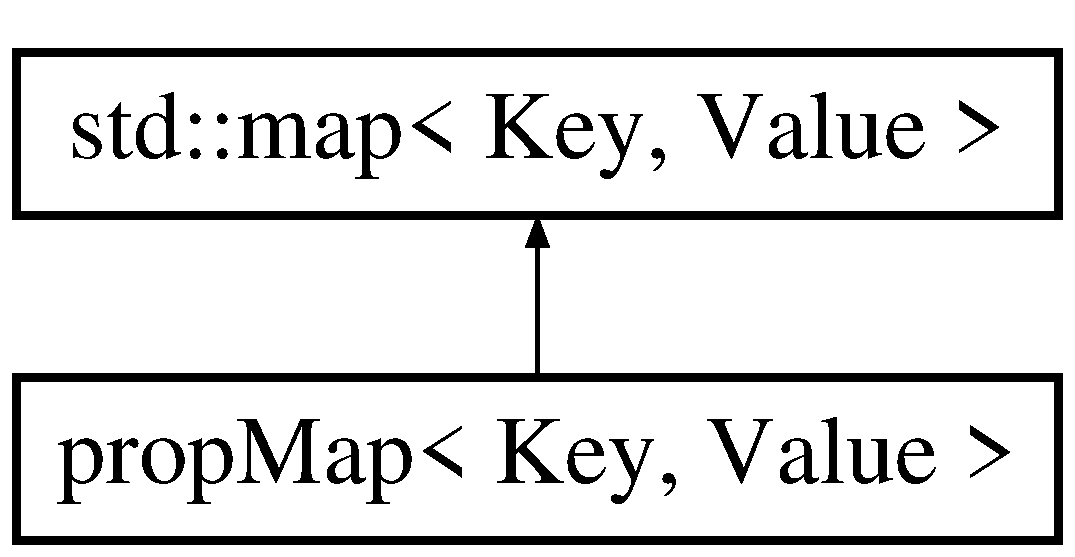
\includegraphics[height=2.000000cm]{classprop_map}
\end{center}
\end{figure}
\subsection*{Public Member Functions}
\begin{DoxyCompactItemize}
\item 
bool \hyperlink{classprop_map_af9969258e92cd7a55002131e2823f5a6}{has\+Key} (const Key \&key) const \hypertarget{classprop_map_af9969258e92cd7a55002131e2823f5a6}{}\label{classprop_map_af9969258e92cd7a55002131e2823f5a6}

\begin{DoxyCompactList}\small\item\em check if it has a specific key? \end{DoxyCompactList}\end{DoxyCompactItemize}


\subsection{Detailed Description}
\subsubsection*{template$<$class Key, class Value$>$\\*
class prop\+Map$<$ Key, Value $>$}

a extended map to store properties 

The documentation for this class was generated from the following file\+:\begin{DoxyCompactItemize}
\item 
N\+C\+T\+U\+Obstacle/include/N\+C\+T\+U\+Obstacle\+Pre\+Requisites.\+h\end{DoxyCompactItemize}

\hypertarget{class_n_c_t_u_1_1_score_bar_window}{}\section{N\+C\+TU\+:\+:Score\+Bar\+Window Class Reference}
\label{class_n_c_t_u_1_1_score_bar_window}\index{N\+C\+T\+U\+::\+Score\+Bar\+Window@{N\+C\+T\+U\+::\+Score\+Bar\+Window}}


G\+UI window for score bar.  




{\ttfamily \#include $<$Score\+Bar\+Window.\+h$>$}

Inheritance diagram for N\+C\+TU\+:\+:Score\+Bar\+Window\+:\begin{figure}[H]
\begin{center}
\leavevmode
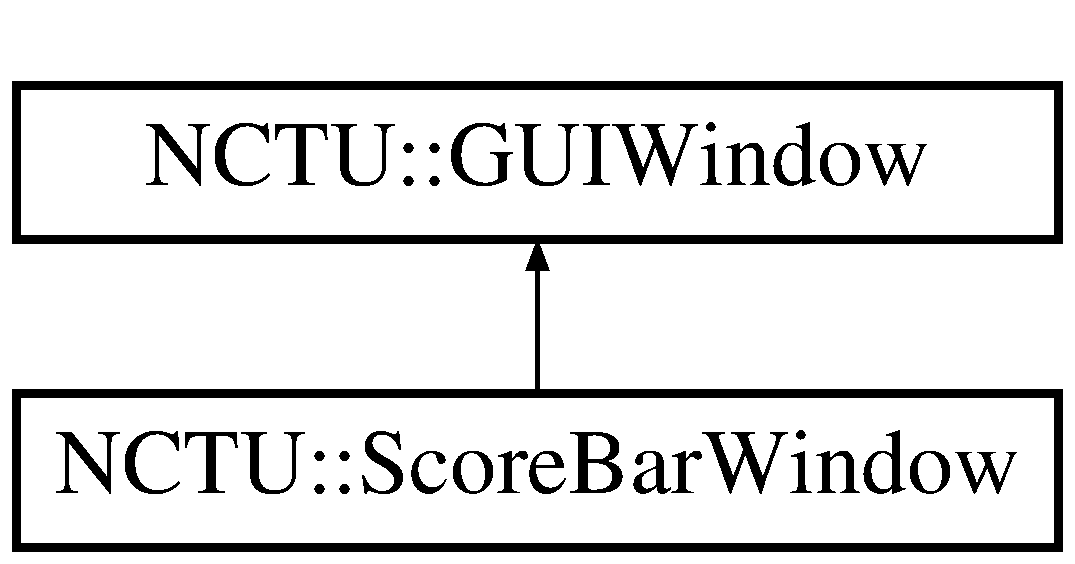
\includegraphics[height=2.000000cm]{class_n_c_t_u_1_1_score_bar_window}
\end{center}
\end{figure}
\subsection*{Public Member Functions}
\begin{DoxyCompactItemize}
\item 
\hyperlink{class_n_c_t_u_1_1_score_bar_window_a1628dea2b5dc856a823064d156d93f3d}{Score\+Bar\+Window} ()\hypertarget{class_n_c_t_u_1_1_score_bar_window_a1628dea2b5dc856a823064d156d93f3d}{}\label{class_n_c_t_u_1_1_score_bar_window_a1628dea2b5dc856a823064d156d93f3d}

\begin{DoxyCompactList}\small\item\em constructor \end{DoxyCompactList}\item 
virtual void \hyperlink{class_n_c_t_u_1_1_score_bar_window_a46c5561d2aced77ed2a3c3766c2f305d}{draw\+Score} (int score)\hypertarget{class_n_c_t_u_1_1_score_bar_window_a46c5561d2aced77ed2a3c3766c2f305d}{}\label{class_n_c_t_u_1_1_score_bar_window_a46c5561d2aced77ed2a3c3766c2f305d}

\begin{DoxyCompactList}\small\item\em draw score on window \end{DoxyCompactList}\item 
virtual void \hyperlink{class_n_c_t_u_1_1_score_bar_window_a603c4e5c83e2aa2b7083d674152f3076}{draw\+Time} (double seconds)\hypertarget{class_n_c_t_u_1_1_score_bar_window_a603c4e5c83e2aa2b7083d674152f3076}{}\label{class_n_c_t_u_1_1_score_bar_window_a603c4e5c83e2aa2b7083d674152f3076}

\begin{DoxyCompactList}\small\item\em draw time on window \end{DoxyCompactList}\item 
virtual void \hyperlink{class_n_c_t_u_1_1_score_bar_window_ac20d65fe5e21a9e516c3a25e7ce4c336}{setup} ()\hypertarget{class_n_c_t_u_1_1_score_bar_window_ac20d65fe5e21a9e516c3a25e7ce4c336}{}\label{class_n_c_t_u_1_1_score_bar_window_ac20d65fe5e21a9e516c3a25e7ce4c336}

\begin{DoxyCompactList}\small\item\em setup everything \end{DoxyCompactList}\item 
virtual void \hyperlink{class_n_c_t_u_1_1_score_bar_window_a7cccdc8832be0d80efdb3907e8483aac}{reset} ()\hypertarget{class_n_c_t_u_1_1_score_bar_window_a7cccdc8832be0d80efdb3907e8483aac}{}\label{class_n_c_t_u_1_1_score_bar_window_a7cccdc8832be0d80efdb3907e8483aac}

\begin{DoxyCompactList}\small\item\em reset the window \end{DoxyCompactList}\end{DoxyCompactItemize}
\subsection*{Protected Attributes}
\begin{DoxyCompactItemize}
\item 
C\+E\+G\+U\+I\+::\+Window $\ast$ \hyperlink{class_n_c_t_u_1_1_score_bar_window_a6bd9be8ccd02bb9954b214806dff87a7}{m\+Score\+Value}\hypertarget{class_n_c_t_u_1_1_score_bar_window_a6bd9be8ccd02bb9954b214806dff87a7}{}\label{class_n_c_t_u_1_1_score_bar_window_a6bd9be8ccd02bb9954b214806dff87a7}

\begin{DoxyCompactList}\small\item\em pointer to the score value sub-\/window \end{DoxyCompactList}\item 
C\+E\+G\+U\+I\+::\+Window $\ast$ \hyperlink{class_n_c_t_u_1_1_score_bar_window_acd0f1e39530c6ce908aea8fdad80d8ec}{m\+Time\+Value}\hypertarget{class_n_c_t_u_1_1_score_bar_window_acd0f1e39530c6ce908aea8fdad80d8ec}{}\label{class_n_c_t_u_1_1_score_bar_window_acd0f1e39530c6ce908aea8fdad80d8ec}

\begin{DoxyCompactList}\small\item\em pointer to the time value sub-\/window \end{DoxyCompactList}\end{DoxyCompactItemize}
\subsection*{Additional Inherited Members}


\subsection{Detailed Description}
G\+UI window for score bar. 

The documentation for this class was generated from the following files\+:\begin{DoxyCompactItemize}
\item 
programs/\+Obstacle/include/Score\+Bar\+Window.\+h\item 
programs/\+Obstacle/source/Score\+Bar\+Window.\+cpp\end{DoxyCompactItemize}

\hypertarget{struct_n_c_t_u_1_1_audio_1_1_sound_slot}{}\section{N\+C\+TU\+:\+:Audio\+:\+:Sound\+Slot Struct Reference}
\label{struct_n_c_t_u_1_1_audio_1_1_sound_slot}\index{N\+C\+T\+U\+::\+Audio\+::\+Sound\+Slot@{N\+C\+T\+U\+::\+Audio\+::\+Sound\+Slot}}


Store information for a single sound playback.  




{\ttfamily \#include $<$N\+C\+T\+U\+Audio.\+h$>$}

\subsection*{Public Member Functions}
\begin{DoxyCompactItemize}
\item 
\hyperlink{struct_n_c_t_u_1_1_audio_1_1_sound_slot_a0639f62320cd31b59cc3d2f55a42eb97}{Sound\+Slot} ()\hypertarget{struct_n_c_t_u_1_1_audio_1_1_sound_slot_a0639f62320cd31b59cc3d2f55a42eb97}{}\label{struct_n_c_t_u_1_1_audio_1_1_sound_slot_a0639f62320cd31b59cc3d2f55a42eb97}

\begin{DoxyCompactList}\small\item\em constrcutor \end{DoxyCompactList}\item 
bool \hyperlink{struct_n_c_t_u_1_1_audio_1_1_sound_slot_a7cd7272636c9801a16e29383181d7ad4}{usable} ()\hypertarget{struct_n_c_t_u_1_1_audio_1_1_sound_slot_a7cd7272636c9801a16e29383181d7ad4}{}\label{struct_n_c_t_u_1_1_audio_1_1_sound_slot_a7cd7272636c9801a16e29383181d7ad4}

\begin{DoxyCompactList}\small\item\em determine this sound slot is usable? \end{DoxyCompactList}\end{DoxyCompactItemize}
\subsection*{Public Attributes}
\begin{DoxyCompactItemize}
\item 
A\+Luint \hyperlink{struct_n_c_t_u_1_1_audio_1_1_sound_slot_add7f3d75354e6750a4085850ec2ab9e6}{buffer}\hypertarget{struct_n_c_t_u_1_1_audio_1_1_sound_slot_add7f3d75354e6750a4085850ec2ab9e6}{}\label{struct_n_c_t_u_1_1_audio_1_1_sound_slot_add7f3d75354e6750a4085850ec2ab9e6}

\begin{DoxyCompactList}\small\item\em Open\+AL buffer. \end{DoxyCompactList}\item 
A\+Luint \hyperlink{struct_n_c_t_u_1_1_audio_1_1_sound_slot_a74c9bb99b1924b4b24955010a3ddc1ff}{source}\hypertarget{struct_n_c_t_u_1_1_audio_1_1_sound_slot_a74c9bb99b1924b4b24955010a3ddc1ff}{}\label{struct_n_c_t_u_1_1_audio_1_1_sound_slot_a74c9bb99b1924b4b24955010a3ddc1ff}

\begin{DoxyCompactList}\small\item\em Open\+AL source. \end{DoxyCompactList}\item 
A\+Lenum \hyperlink{struct_n_c_t_u_1_1_audio_1_1_sound_slot_ab146746f7f9e8a1c8c9724efc4c04b9d}{error}\hypertarget{struct_n_c_t_u_1_1_audio_1_1_sound_slot_ab146746f7f9e8a1c8c9724efc4c04b9d}{}\label{struct_n_c_t_u_1_1_audio_1_1_sound_slot_ab146746f7f9e8a1c8c9724efc4c04b9d}

\begin{DoxyCompactList}\small\item\em Open\+AL error. \end{DoxyCompactList}\item 
A\+Lint \hyperlink{struct_n_c_t_u_1_1_audio_1_1_sound_slot_a65f64b644c4e89f9a315dc9c56dd5e56}{status}\hypertarget{struct_n_c_t_u_1_1_audio_1_1_sound_slot_a65f64b644c4e89f9a315dc9c56dd5e56}{}\label{struct_n_c_t_u_1_1_audio_1_1_sound_slot_a65f64b644c4e89f9a315dc9c56dd5e56}

\begin{DoxyCompactList}\small\item\em Open\+AL status code. \end{DoxyCompactList}\item 
bool \hyperlink{struct_n_c_t_u_1_1_audio_1_1_sound_slot_ab61836c67fcb5f72d147dd64b6f5997e}{used}\hypertarget{struct_n_c_t_u_1_1_audio_1_1_sound_slot_ab61836c67fcb5f72d147dd64b6f5997e}{}\label{struct_n_c_t_u_1_1_audio_1_1_sound_slot_ab61836c67fcb5f72d147dd64b6f5997e}

\begin{DoxyCompactList}\small\item\em whether this sound clip is in use \end{DoxyCompactList}\end{DoxyCompactItemize}


\subsection{Detailed Description}
Store information for a single sound playback. 

The documentation for this struct was generated from the following files\+:\begin{DoxyCompactItemize}
\item 
N\+C\+T\+U\+Audio/include/N\+C\+T\+U\+Audio.\+h\item 
N\+C\+T\+U\+Audio/source/N\+C\+T\+U\+Audio.\+cpp\end{DoxyCompactItemize}

\hypertarget{class_n_c_t_u_1_1_sphere_obstacle}{}\section{N\+C\+TU\+:\+:Sphere\+Obstacle Class Reference}
\label{class_n_c_t_u_1_1_sphere_obstacle}\index{N\+C\+T\+U\+::\+Sphere\+Obstacle@{N\+C\+T\+U\+::\+Sphere\+Obstacle}}


sphere obstacle for testing  




{\ttfamily \#include $<$N\+C\+T\+U\+Sphere\+Obstacle.\+h$>$}

Inheritance diagram for N\+C\+TU\+:\+:Sphere\+Obstacle\+:\begin{figure}[H]
\begin{center}
\leavevmode
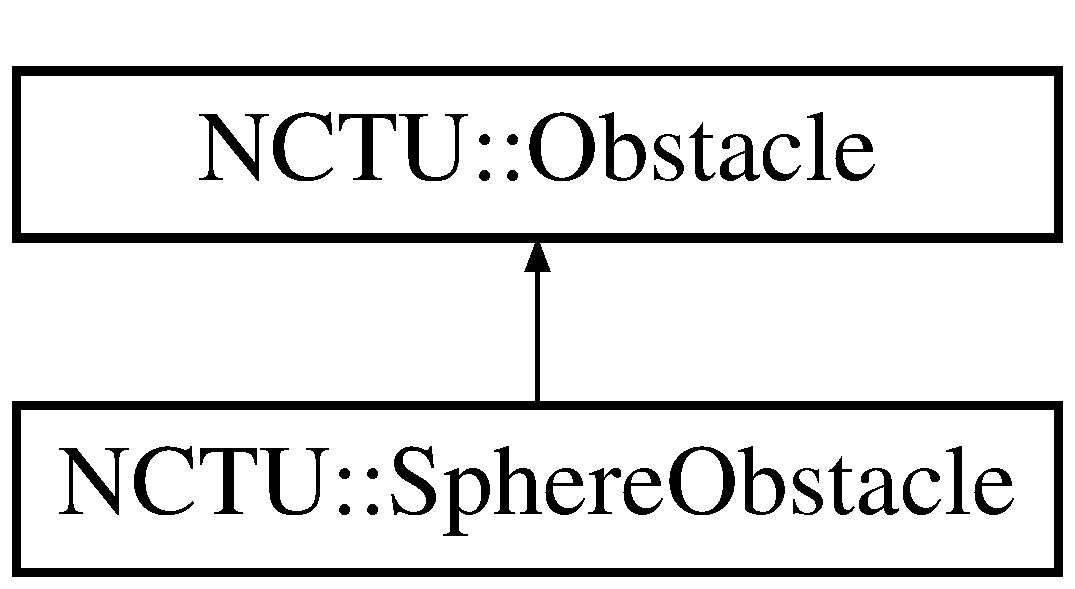
\includegraphics[height=2.000000cm]{class_n_c_t_u_1_1_sphere_obstacle}
\end{center}
\end{figure}
\subsection*{Public Member Functions}
\begin{DoxyCompactItemize}
\item 
\hyperlink{class_n_c_t_u_1_1_sphere_obstacle_aab3b59f8a8426743205288bc3f577462}{Sphere\+Obstacle} (\hyperlink{class_n_c_t_u_1_1_obstacle_manager}{Obstacle\+Manager} $\ast$mgmt, Ogre\+::\+Real restitution, Ogre\+::\+Real friction, Ogre\+::\+Real mass, I\+N\+D\+E\+X\+\_\+\+T\+Y\+PE index, const Ogre\+::\+Vector3 \&position, Ogre\+::\+Real radius, const Ogre\+::\+Quaternion \&orientation)
\begin{DoxyCompactList}\small\item\em constructor \end{DoxyCompactList}\item 
virtual void \hyperlink{class_n_c_t_u_1_1_sphere_obstacle_afb4c3cd47a6482abc858c64078658163}{set\+Scale} (const Ogre\+::\+Vector3 \&)\hypertarget{class_n_c_t_u_1_1_sphere_obstacle_afb4c3cd47a6482abc858c64078658163}{}\label{class_n_c_t_u_1_1_sphere_obstacle_afb4c3cd47a6482abc858c64078658163}

\begin{DoxyCompactList}\small\item\em set scale for this object \end{DoxyCompactList}\end{DoxyCompactItemize}
\subsection*{Protected Attributes}
\begin{DoxyCompactItemize}
\item 
I\+N\+D\+E\+X\+\_\+\+T\+Y\+PE \hyperlink{class_n_c_t_u_1_1_sphere_obstacle_a4855c1addf0ce775a6bd5be08792766c}{m\+Index}\hypertarget{class_n_c_t_u_1_1_sphere_obstacle_a4855c1addf0ce775a6bd5be08792766c}{}\label{class_n_c_t_u_1_1_sphere_obstacle_a4855c1addf0ce775a6bd5be08792766c}

\begin{DoxyCompactList}\small\item\em the object index \end{DoxyCompactList}\item 
Ogre\+::\+Real \hyperlink{class_n_c_t_u_1_1_sphere_obstacle_a57da3759dbbd26ccbd257977fe777e9c}{m\+Radius}\hypertarget{class_n_c_t_u_1_1_sphere_obstacle_a57da3759dbbd26ccbd257977fe777e9c}{}\label{class_n_c_t_u_1_1_sphere_obstacle_a57da3759dbbd26ccbd257977fe777e9c}

\begin{DoxyCompactList}\small\item\em sphere radius \end{DoxyCompactList}\end{DoxyCompactItemize}
\subsection*{Additional Inherited Members}


\subsection{Detailed Description}
sphere obstacle for testing 

\subsection{Constructor \& Destructor Documentation}
\index{N\+C\+T\+U\+::\+Sphere\+Obstacle@{N\+C\+T\+U\+::\+Sphere\+Obstacle}!Sphere\+Obstacle@{Sphere\+Obstacle}}
\index{Sphere\+Obstacle@{Sphere\+Obstacle}!N\+C\+T\+U\+::\+Sphere\+Obstacle@{N\+C\+T\+U\+::\+Sphere\+Obstacle}}
\subsubsection[{\texorpdfstring{Sphere\+Obstacle(\+Obstacle\+Manager $\ast$mgmt, Ogre\+::\+Real restitution, Ogre\+::\+Real friction, Ogre\+::\+Real mass, I\+N\+D\+E\+X\+\_\+\+T\+Y\+P\+E index, const Ogre\+::\+Vector3 \&position, Ogre\+::\+Real radius, const Ogre\+::\+Quaternion \&orientation)}{SphereObstacle(ObstacleManager *mgmt, Ogre::Real restitution, Ogre::Real friction, Ogre::Real mass, INDEX_TYPE index, const Ogre::Vector3 &position, Ogre::Real radius, const Ogre::Quaternion &orientation)}}]{\setlength{\rightskip}{0pt plus 5cm}Sphere\+Obstacle\+::\+Sphere\+Obstacle (
\begin{DoxyParamCaption}
\item[{{\bf Obstacle\+Manager} $\ast$}]{mgmt, }
\item[{Ogre\+::\+Real}]{restitution, }
\item[{Ogre\+::\+Real}]{friction, }
\item[{Ogre\+::\+Real}]{mass, }
\item[{I\+N\+D\+E\+X\+\_\+\+T\+Y\+PE}]{index, }
\item[{const Ogre\+::\+Vector3 \&}]{position, }
\item[{Ogre\+::\+Real}]{radius, }
\item[{const Ogre\+::\+Quaternion \&}]{orientation}
\end{DoxyParamCaption}
)}\hypertarget{class_n_c_t_u_1_1_sphere_obstacle_aab3b59f8a8426743205288bc3f577462}{}\label{class_n_c_t_u_1_1_sphere_obstacle_aab3b59f8a8426743205288bc3f577462}


constructor 

Create a sphere obstacle (full) 

The documentation for this class was generated from the following files\+:\begin{DoxyCompactItemize}
\item 
N\+C\+T\+U\+Obstacle/include/N\+C\+T\+U\+Sphere\+Obstacle.\+h\item 
N\+C\+T\+U\+Obstacle/src/N\+C\+T\+U\+Sphere\+Obstacle.\+cpp\end{DoxyCompactItemize}

%--- End generated contents ---

% Index
\backmatter
\newpage
\phantomsection
\clearemptydoublepage
\addcontentsline{toc}{chapter}{Index}
\printindex

\end{document}
